\documentclass[11pt,]{article}
\usepackage[left=1in,top=1in,right=1in,bottom=1in]{geometry}
\newcommand*{\authorfont}{\fontfamily{phv}\selectfont}
\usepackage[]{mathpazo}


  \usepackage[T1]{fontenc}
  \usepackage[utf8]{inputenc}



\usepackage{abstract}
\renewcommand{\abstractname}{}    % clear the title
\renewcommand{\absnamepos}{empty} % originally center

\renewenvironment{abstract}
 {{%
    \setlength{\leftmargin}{0mm}
    \setlength{\rightmargin}{\leftmargin}%
  }%
  \relax}
 {\endlist}

\makeatletter
\def\@maketitle{%
  \newpage
%  \null
%  \vskip 2em%
%  \begin{center}%
  \let \footnote \thanks
    {\fontsize{18}{20}\selectfont\raggedright  \setlength{\parindent}{0pt} \@title \par}%
}
%\fi
\makeatother




\setcounter{secnumdepth}{3}

\usepackage{longtable,booktabs}

\usepackage{graphicx,grffile}
\makeatletter
\def\maxwidth{\ifdim\Gin@nat@width>\linewidth\linewidth\else\Gin@nat@width\fi}
\def\maxheight{\ifdim\Gin@nat@height>\textheight\textheight\else\Gin@nat@height\fi}
\makeatother
% Scale images if necessary, so that they will not overflow the page
% margins by default, and it is still possible to overwrite the defaults
% using explicit options in \includegraphics[width, height, ...]{}
\setkeys{Gin}{width=\maxwidth,height=\maxheight,keepaspectratio}

\title{Análisis de la familia de plantas Malvaceae en la parcela de 50
Hectáreas de la Isla Barro Colorado, Panamá.  }



\author{\Large Carolain Pérez Ureña\vspace{0.05in} \newline\normalsize\emph{Estudiante, Universidad Autónoma de Santo Domingo (UASD)}  }


\date{}

\usepackage{titlesec}

\titleformat*{\section}{\normalsize\bfseries}
\titleformat*{\subsection}{\normalsize\itshape}
\titleformat*{\subsubsection}{\normalsize\itshape}
\titleformat*{\paragraph}{\normalsize\itshape}
\titleformat*{\subparagraph}{\normalsize\itshape}

\titlespacing{\section}
{0pt}{36pt}{0pt}
\titlespacing{\subsection}
{0pt}{36pt}{0pt}
\titlespacing{\subsubsection}
{0pt}{36pt}{0pt}





\newtheorem{hypothesis}{Hypothesis}
\usepackage{setspace}

\makeatletter
\@ifpackageloaded{hyperref}{}{%
\ifxetex
  \PassOptionsToPackage{hyphens}{url}\usepackage[setpagesize=false, % page size defined by xetex
              unicode=false, % unicode breaks when used with xetex
              xetex]{hyperref}
\else
  \PassOptionsToPackage{hyphens}{url}\usepackage[unicode=true]{hyperref}
\fi
}

\@ifpackageloaded{color}{
    \PassOptionsToPackage{usenames,dvipsnames}{color}
}{%
    \usepackage[usenames,dvipsnames]{color}
}
\makeatother
\hypersetup{breaklinks=true,
            bookmarks=true,
            pdfauthor={Carolain Pérez Ureña (Estudiante, Universidad Autónoma de Santo Domingo (UASD))},
             pdfkeywords = {Malvaceae, ecología espacial, variables ambientales, especies, BCI,
Quararibea asterolepis},  
            pdftitle={Análisis de la familia de plantas Malvaceae en la parcela de 50
Hectáreas de la Isla Barro Colorado, Panamá.},
            colorlinks=true,
            citecolor=blue,
            urlcolor=blue,
            linkcolor=magenta,
            pdfborder={0 0 0}}
\urlstyle{same}  % don't use monospace font for urls

% set default figure placement to htbp
\makeatletter
\def\fps@figure{htbp}
\makeatother

\usepackage{pdflscape} \newcommand{\blandscape}{\begin{landscape}}
\newcommand{\elandscape}{\end{landscape}} \usepackage{float}
\floatplacement{figure}{H}
\newcommand{\beginsupplement}{ \setcounter{table}{0} \renewcommand{\thetable}{S\arabic{table}} \setcounter{figure}{0} \renewcommand{\thefigure}{S\arabic{figure}} }


% add tightlist ----------
\providecommand{\tightlist}{%
\setlength{\itemsep}{0pt}\setlength{\parskip}{0pt}}

\begin{document}
	
% \pagenumbering{arabic}% resets `page` counter to 1 
%
% \maketitle

{% \usefont{T1}{pnc}{m}{n}
\setlength{\parindent}{0pt}
\thispagestyle{plain}
{\fontsize{18}{20}\selectfont\raggedright 
\maketitle  % title \par  

}

{
   \vskip 13.5pt\relax \normalsize\fontsize{11}{12} 
\textbf{\authorfont Carolain Pérez Ureña} \hskip 15pt \emph{\small Estudiante, Universidad Autónoma de Santo Domingo (UASD)}   

}

}








\begin{abstract}

    \hbox{\vrule height .2pt width 39.14pc}

    \vskip 8.5pt % \small 

\noindent La Isla Barro Colorado más conocida como BCI (por sus siglas en inglés)
se caracteriza por ser un lugar idóneo para la realización de estudios
cientificos. Tal es el caso de esta investigación donde se estudió la
familia de planta \emph{Malvaceae} perteneciente a la parcela de 50
hectárea de la Isla. Este tuvo como objetivo analizar la riqueza,
abundancia, asociación, agrupamiento de datos, distribución, y
autocorrelación entre las variables de la familia \emph{Malvaceae}. Así
como verificar si existe una relación entre los factores ambientales
(elementos del suelo y relieve) con su patrón de distribución y
asociación. También busca identificar las especies consideradas como
indicadoras, las especies que más contribuyeron a la diversidad (alpha y
beta) y distinguir los sitios con mayor y menor abundancia. Evaluar la
colinealidad entre las variables del suelo y especies con técnicas de
ordenación e identificar concretamente cuáles son las especies,
elementos químicos de suelo y área geomorfológica más significativos en
la distribución, diversidad, autocorrelación espacial, y en su
homogeneidad. Mediante métricas y con datos de censos recolectados
durante años se obtuvieron los resultados esperados. De este modo, se
determinó el comportamiento de la familia de plantas \emph{Malvaceae} en
la parcela, así como los factores ambientales, del relieve y elementos
del suelo que intervienen en dicho comportamiento.


\vskip 8.5pt \noindent \emph{Keywords}: Malvaceae, ecología espacial, variables ambientales, especies, BCI,
Quararibea asterolepis \par

    \hbox{\vrule height .2pt width 39.14pc}



\end{abstract}


\vskip 6.5pt


\noindent  \section{Introducción}\label{introducciuxf3n}

Una de las áreas naturales más estudiadas por los cientificos durante
años ha sido la isla Barro Colorado (BCI) localizada en el lago Gatún
del canal de Panamá. Su diversidad de bosques y su fauna la han
convertido en un centro de estudio, útil para hacer proyectos de
exploración. Es considerada como uno de los sitios con más larga
historia de investigación continua en los trópicos del Nuevo Mundo, lo
que ha proporcionado una base de información científica inigualada en
todo el planeta. Cada año, entre 200 y 400 científicos de todo el mundo
visitan el Monumento Natural Barro Colorado.(Fisher, 2016)

La mitad de la isla se encuentra cubierta de bosque jóven tropical
húmedo semi-perenne de 100 o más años de edad, el resto está cubierto de
bosque viejo el cual ha sufrido muy pocas perturbaciones en los últimos
400 años (Moreno, 2012). Se caracteriza por tener un promedio anual de
temperatura de 27\(^{\circ}\) C en áreas abiertas, con una variación
diurna de 9\(^{\circ}\) C. Tiene una precipitación promedio anual es de
2,600 mm, con una estación lluviosa que va de mayo a diciembre, y una
estación seca que comprende los meses restantes. Está constituida por un
total de 265 especies de plantas, y cada una pertenece a una familia.
(Croat, 1978).

Dentro de su amplia variedad de familias de plantas se encuentran las
\emph{Malvaceae}. Esta planta pertenece a la familia de las
\emph{Malvales}, que reúne cerca de 250 géneros y 3929 especies
distribuidas por las regiones templadas y cálidas de todo el mundo
(Rondón, 2009).

Son plantas de hierbas, arbustos o árboles, generalmente con pelos
estrellados. Los tallos son de fibra de líber robusta con cavidad de
mucílago. Las hojas son simples, alternas,palmadamente divididas,
palmadas veteadas, con estípulas y pecioladas. Las flores son
actinomórficas, solitarias, fasciculadas o dispuestas en cimas o
panículas con sépalos de 3 a 5, libres o connatos y valvados. Los
pétalos son cinco, libres, giratorios, adnados a la columna estaminal en
la base. Los estambres son numerosos, filamentos connados en tubos,
conocidos como adelfos (Xu \& Deng, 2017)(ver figura \ref{Figura}).

\begin{figure}
\centering
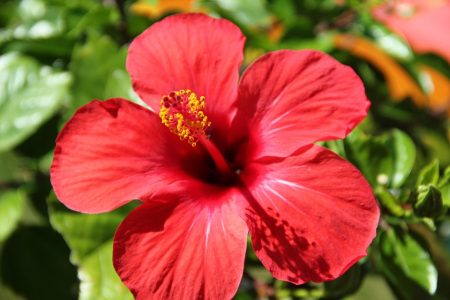
\includegraphics[width=0.50000\textwidth]{Hibiscus-Malvaceae.jpg}
\caption{Flor de la planta Malvaceae \label{Figura}}
\end{figure}

Barro Colorado ofrece ventajas excepcionales para un estudio de
ecología, y la morfología de ciertos grupos de plantas podría
investigarse provechosamente (Standley, 1927). Razón, por la que el
presente estudio se basó en analizar el comportamiento de la familia de
plantas \emph{Malvaceae} en BCI; en el cual abarcó un análisis de
abundancia, riqueza, asociación, distribución, agrupamiento,
autocorrelación espacial entre las variables de la familia y la
influencia que tienen los factores ambientales y geomorfológicos en su
patrón de distribución y asociación.

De igual forma, con el análisis de diversidad (alpha y beta) conocer la
riqueza y equidad de las especies junto con los sitios que tienen mayor
y menor diversidad. Además de, conocer las especies consideradas como
indicadoras, y determinar la colinealidad existente entre variables del
suelo especies.

Por último, identificar cuáles son las especies, elementos del suelo y
áreas morfológicas más significativos en la distribución, diversidad,
autocorrelación espacial, y en su homogeneidad. Por otro lado, se busca
conocer el método más eficiente para agrupar y organizar los datos a
través de dendogramas. Esta investigación podrá ser utilizada como base
para estudios posteriores con esta importante familia de plantas.

\section{Metodología}\label{metodologuxeda}

\emph{Área de estudio y descripción de metodología}

El estudio se realizó en la Isla Barro Colorado (BCI), localizada entre
los 9\(^{\circ}\) 09' N y 79\(^{\circ}\) 51' W, que forma parte del
Monumento Natural de Barro Colorado (5,500 ha, Leigh, 1999). Formada en
1914 cuando se represó el Río Gatún como parte del trabajo para la
creación del Canal de Panamá (Moreno, 2012). Es una zona administrada
por el Instituto de Investigaciones Tropicales del Smithsonian dedicada
a investigaciones científicas.

Dentro de Isla se encuentra la parcela de 50 Hectáreas con 1,000 metros
de largo y 500 metros de ancho lo que da un total de 50 ha que se
subdivide en 1 ha. En la que se llevó a cabo el presente estudio (ver
figura \ref{mapa_1}).

\begin{figure}
\centering
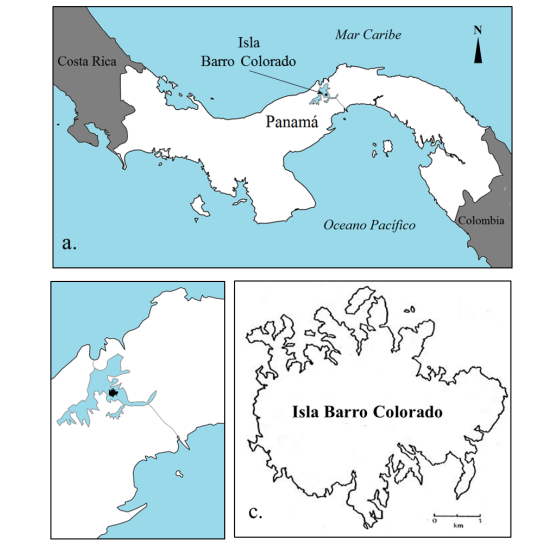
\includegraphics[width=0.50000\textwidth]{isla_barro_colorado_mapa.png}
\caption{Mapa de la Isla Barro Colorado \label{mapa_1}}
\end{figure}

La mayor parte del trabajo se desarrolló en entorno al lenguaje de
programación R, en el cuál se efectuaron los análisis de agrupamientos,
ambientales, ordenamiento y de ecología numérica, apoyandose con
paquetes como \emph{tidyverse} junto con \emph{dplyr} y \emph{vegan} con
la cual se crearon las matrices de comunidad ambientales. Con el paquete
\emph{simple features} (sf) se crearon cuadros por hectáreas para así
obtener la densidad de cada especie. En menor medida se emplearon los
paquetes \emph{adespatial}, \emph{vegetarian}, \emph{broom} y
\emph{cluster}. Paquetes como \emph{ez} fueron usados para la
correlación entre variables y \emph{ggplot2}, \emph{mapview} y
\emph{graphics} para la representación gráfica. Los datos se obtuvieron
a partir del repositorio de ecología númerica de José Martinez Battle
(Batlle, 2020)(2020).

En la primera etapa del trabajo se efectuó un análisis ambiental de
asociación estadística con los datos pre-censales de la parcela de BCI,
usando una matriz de comunidad convertidas en columnas de hábitats para
generar mapas de abundancia por especie, y riqueza numérica de toda la
comunidad.

Para el análisis de asociación se usaron las métricas de modo Q y R; con
el coeficiente de correlación de Pearson que mide la relación
estadística entre dos variables. En cuanto a la medición de asociación
de distancia entre sitios; se usó la transformación de la matriz de
Hellinger con la metodología de la similaridad de Jaccard para obtener
una matriz de distancia de comunidad transformada a la cuál se le
calculó su distancia euclidea la cual indica que mientras mayor
distancia menor similaridad, es decir, mientras más crece la distancia
el parecido entre los sitios es cada vez menor.

La segunda fase del trabajo se basó en el análisis de agrupamiento. Con
el fin de comprobar el método más adecuado para agrupar las especies en
forma de dendograma se compararon los métodos de por enlace simple,
completo, de grupo de pares ponderados con media aritmética conocido
como UPGMA (siglas de \emph{unweighted pair group method with arithmetic
mean}) y el método Ward teniendo como criterio la correlación
cofenética.

Con los valores de abundancia de especie junto con el método de varianza
mínima de agrupamiento de Ward se construyó un árbol dentrítico tomando
el criterio de la técnica de anchura de silueta, que refleja los cortes
del arbol en varios grupos usando la posición que ocupa el promedio más
alto. Para obtener resultados más fiables se usó el reemuestreo de
boostrap multiescalar que permite resolver problemas relacionados con la
estimación de intervalos de confianza o la prueba de significación
estadística (Ledesma, 2008).

Por medio de la prueba \emph{t} de \emph{Student}, y la prueba no
paramétrica de la suma de rangos de Wilcoxon (medianas), se evaluaron la
homogeneidad de medias y medianas para dos grupos usando como variable
de agrupamiento los grupos establecidos en el agrupamiento Ward. Estas
sirvieron para hacer una correlación con los resultados de abundancia la
global y la de la especie.

Mediante el valor indicador (indVal) se detectaron las especies
consideradas como indicadoras y un análisis de especies con preferencia
por hábitat por medio del coeficiente de correlación biserial puntual.

Utilizando la técnica del análisis de componentes principales (PCA) y
técnica de ordenación restrigida de analisis de abundancia o RDA (siglas
de \emph{Redundancy Analysis}) y canónica por la prueba de \emph{Chi}
cuadrado. Se comprobó la coleidalidad entre las variables del suelo y
tipos de especies y reconocer la especies más contribuidora, esto se
realizó por el criterio de valores señalados con \emph{VIF}.

Para la tercera etapa se midió la de diversidad (alpha y beta) donde se
determinaron dos componentes principales; la riqueza y equidad. Por
medio de la entropia de Shannon y la antripia de Simpson se midió el
indice de equidad de Pielu para la diversidad alpha.En el análisis beta
se buscó la equidad usando la aproximación de Whittaker, asociada a los
números de Hill y la ratio. Se identificaron las especie y sitios que
contribuyen a la diversidad beta. También, se utilizó el método de la
rarefacción para poder estimar combinaciones se utilizaron las métricas
de la entropia de Renyi generaliza para obtienen los números de
diversidad de Hill.

En la última etapa, basada fundamentalmente en ecología espacial se
llevaron a cabo análisis de autocorrelación espacial mediante
correlograma de puntos y correlación. Así las técnicas aplicadas fueron
la de mantel para determinar la correlación entre dos matrices de
distancia y determinar autocorrelación mediante la prueba de permutación
para \emph{I} de \emph{moran}, utilizando los denominados Lisa.

\section{Resultados}\label{resultados}

La familia de plantas \emph{Malvaceae} cuenta con una cantidad de 3,792
individuos dentro de la parcela (Ver Tabla 1). En promedio la cantidad
de especies por hectárea ronda en torno a unas 8 individuos.

A simple vista en la figura presentada más abajo la especie más
abundante del conjunto es \emph{Quararibea asterolepis} guardando una
similitud con el resto de las especies (Ver figura \ref{agrupado}).

\begin{longtable}[]{@{}ll@{}}
\toprule
Especies de planta & Cantidad\tabularnewline
\midrule
\endhead
Quararibea asterolepis & 2171\tabularnewline
Herrania purpurea & 542\tabularnewline
Apeiba membranacea & 308\tabularnewline
Luehea seemannii & 215\tabularnewline
Hampea appendiculata & 191\tabularnewline
Guazuma ulmifolia & 74\tabularnewline
Ceiba pentandra & 62\tabularnewline
Sterculia apetala & 53\tabularnewline
Apeiba tibourbou & 50\tabularnewline
Pseudobombax septenatum & 42\tabularnewline
Cavanillesia platanifolia & 36\tabularnewline
Pachira sessilis & 18\tabularnewline
Theobroma cacao & 16\tabularnewline
Ochroma pyramidale & 11\tabularnewline
Trichospermum galeottii & 2\tabularnewline
Pachira quinata & 1\tabularnewline
\bottomrule
\end{longtable}

Tabla 1.Abundancia por especies

\begin{figure}
\centering
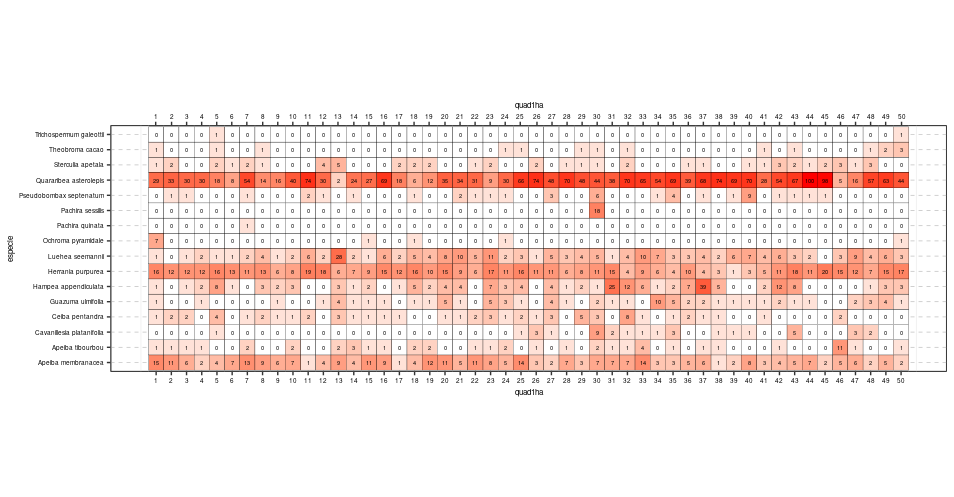
\includegraphics[width=1.00000\textwidth]{mosaico_abundancia.png}
\caption{Gráfico de mosaico de abundancia por especie\label{agrupado}}
\end{figure}

Al evaluar la primera etapa del estudio basado en el análisis ambiental
se refleja que en la parte oriental de la parcela existe una mayor
abundancia de la familia \emph{Malvaceae} y una distribución de riquezas
máximas concentrada en el borde superior central (Ver figura
\ref{mapa_abundancia} y \ref{mapa_riqueza}).

\begin{figure}
\centering
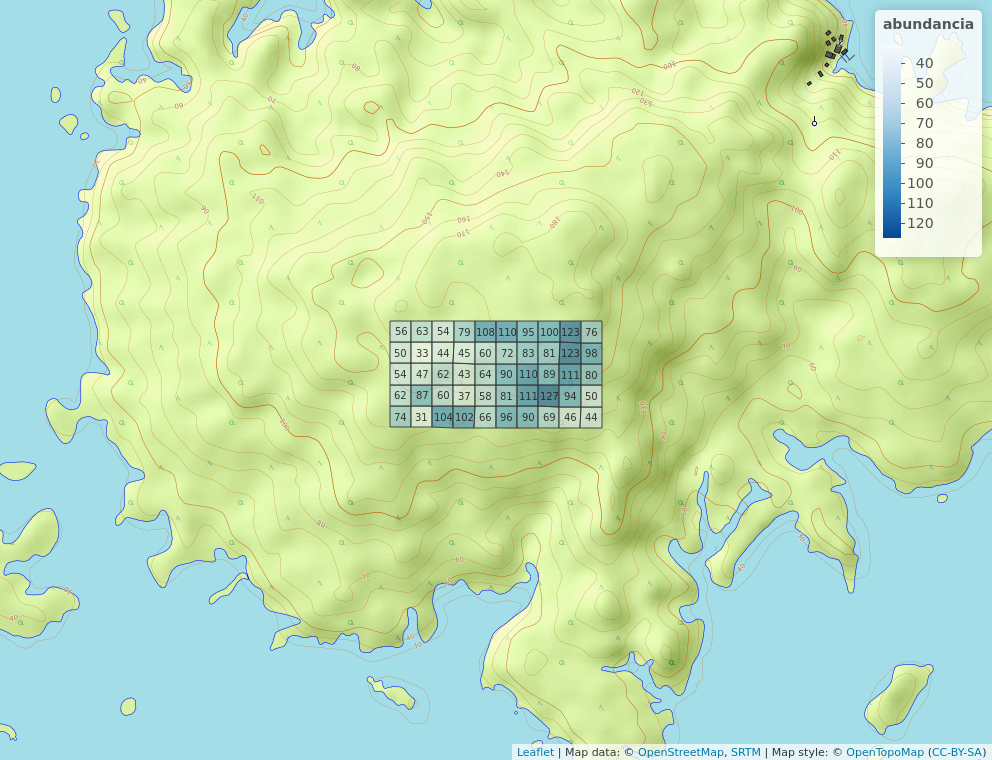
\includegraphics[width=0.80000\textwidth]{mapa_cuadros_abun_mi_familia.png}
\caption{Distribución de la abundancia por cuadros de la familia
Malvaceae por Ha \label{mapa_abundancia}}
\end{figure}

\begin{figure}
\centering
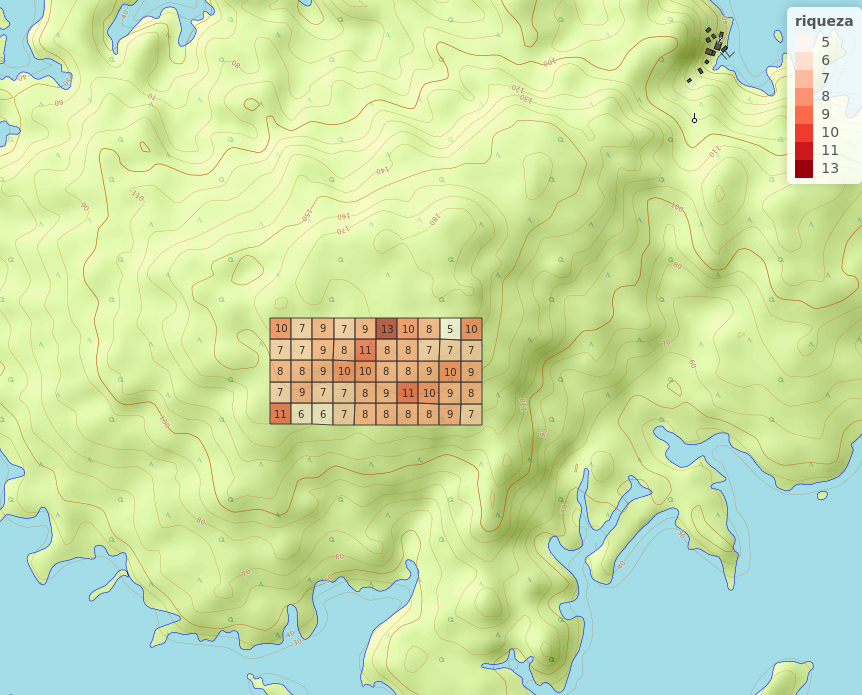
\includegraphics[width=0.80000\textwidth]{mapa_cuadros_riq_mi_familia.png}
\caption{Districución de las riquezas por cuadros de 1 Ha
\label{mapa_riqueza}}
\end{figure}

\subsection{Análisis de asociación}\label{anuxe1lisis-de-asociaciuxf3n}

En el mapa de calor ordenado (a la derecha), presenta un clúster gigante
en el centro que indica un patrón ordenado de dependencia entre las
especies relacionadas. En la diagonal desde \emph{Pseudobombax
septenatum} hasta \emph{Apeiba tibourbou} (cuadros de color rosa
centrales). También se observan las especies que no parecen asociarse
con otras, situadas en los extremos de la diagonal, y relacionadas con
otras por medio de valores pequeños de distancia (cuadros azules), como
\emph{Theobroma cacao} y \emph{Pachira sessilis}.El color rosado indica
distancia corta y mientras más cortas los cluster se parecen entre sí
(Ver figura \ref{fig:representacion_asociación_Jaccard}).

\begin{figure}
\centering
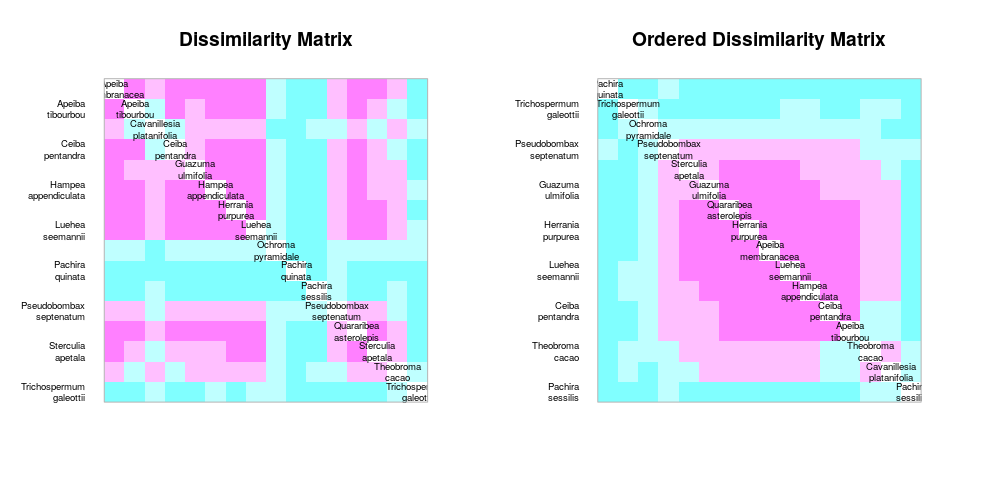
\includegraphics[height=5.00000\textwidth]{Asociacion_variables_jaccard.png}
\caption{Matriz de asociación entre especies
\label{fig:representacion_asociación_Jaccard}}
\end{figure}

\subsection{Análisis de agrupamiento}\label{anuxe1lisis-de-agrupamiento}

Los dendogramas fueron generados por los métodos de enlaces simple,
completos, UGMA y Ward (Ver figura \ref{4_dendogramas}). Estos mostraron
cortes desiguales en los método UPGMA, completo y simple produciendo
agrupamientos integrados por un gran número de sitios o por un sitio
único. Se detectaron elementos que no forman grupos, es decir, sitios
que aparecen aislados del resto como fue el caso del método por enlace
simple. No obstante, con el método Ward de anchura de silueta se generó
un dendograma más legible. Dicho método sugirió dividir el dendograma en
2 grupos; un grupo pequeño integrado por 8 sitios y otro grupo compuesto
por los 42 sitios restantes (Ver figura \ref{dendograma_ward}).

\begin{figure}
\centering
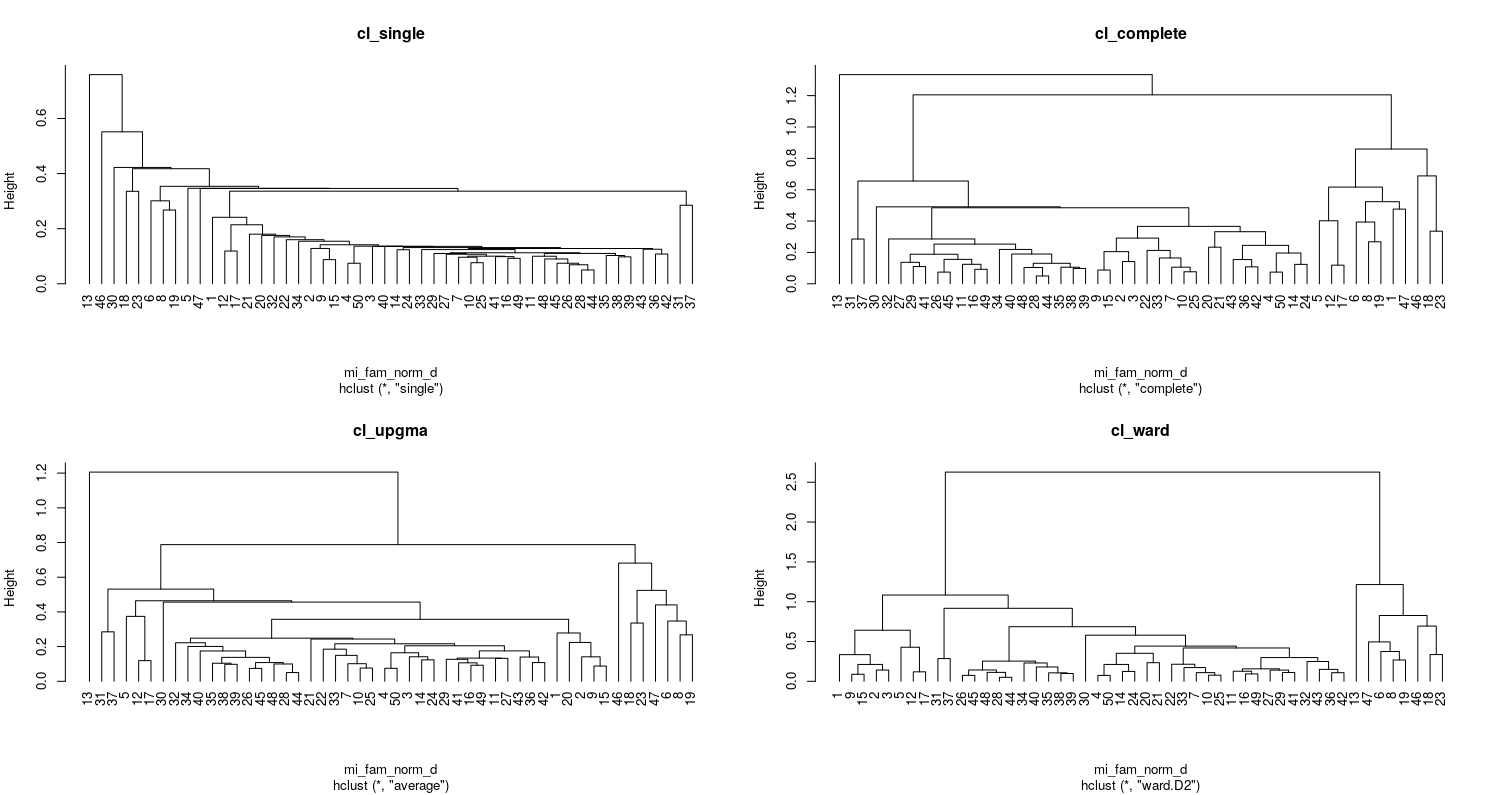
\includegraphics[width=1.10000\textwidth]{4_dendogramas.png}
\caption{Dendogramas por los cuatro métodos \label{dendogramas}}
\end{figure}

\begin{figure}
\centering
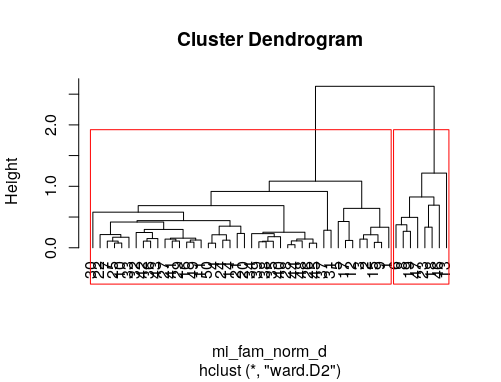
\includegraphics[width=0.80000\textwidth]{dendograma_metodo_ward_2_grupos.png}
\caption{Dendograma por el método Ward \label{dendograma_ward}}
\end{figure}

Para la homogeneidad de promedios se evaluaron mediante las pruebas
\emph{T} de \emph{Student} y la suma de rango de Wilcoxon por el métodos
de Ward divididas en dos grupos. Estos paneles muestran el promedio
entre las variables geomorfológicas y elementos del suelo. El nitrógeno
(N), pH,cobre (Cu), y magnesio (Mg) y zinc (Zn) resultaron ser
significativamente diferentes en media y mediana; en el caso del relieve
el la pendiente media resultó tener el promedio más diferente, en cambio
los elementos con mayor homegeneidad de medianas fueron el boro (B),
manganeso (Mn), y potasio(K) y en las áreas de relieve estuvieron la
elevación media, espolón, e interfluvio (ver figura \ref{homogeneidad}).

Por medio del método del ``valor indicador'' (Indval), se encontraron en
total 3 especies que pueden ser consideradas como indicadoras con
preferencia de habitats. Especificamente estas especies fueron
\emph{Quararibea asterolepis} como especie asociada al grupo 1,
\emph{Luehea seemannii} y \emph{Sterculia apetala} pertenecientes al
grupo 2, lo significa que estas especies son extremadamente importantes
en la prueba de permutación.

\begin{figure}
\centering
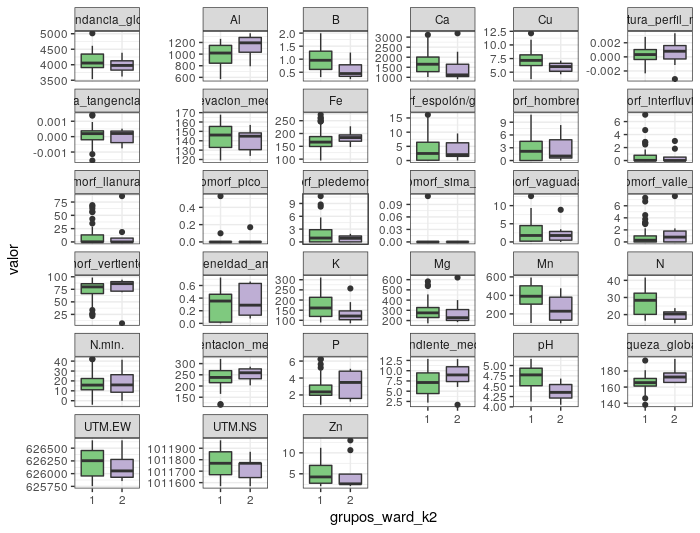
\includegraphics[width=0.90000\textwidth]{Homogeneidad_promedios_ward.png}
\caption{Pruebas de igualdad de promedios entre las variables
\label{homogeneidad}}
\end{figure}

\subsection{Técnicas de ordenación}\label{tuxe9cnicas-de-ordenaciuxf3n}

En el analisis de correspondencia por el método PCA, al ajustarlo a la
matriz de comunidad y usando la distancia \emph{Chi} cuadrado, se
encuentra que muchos de los componentes del suelo se encuentran
asociados en las variables de comunidad, por lo que, presentan algún
grado de asociación entre las especies.(Ver figura
\ref{escalonamiento}).

\begin{figure}
\centering
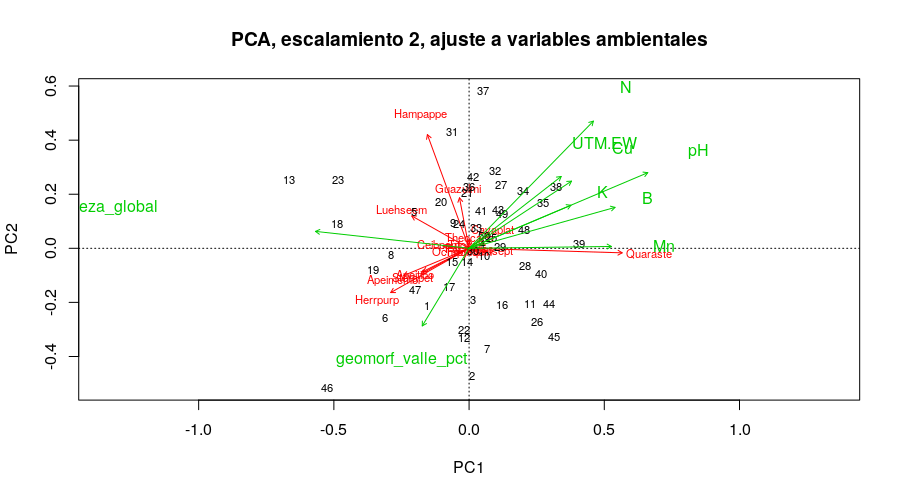
\includegraphics[width=1.00000\textwidth]{Escalonamiento_ajustado_variables_ambientales.png}
\caption{Biplot de variables ambientales por el método PCA
\label{escalonamiento}}
\end{figure}

\begin{figure}
\centering
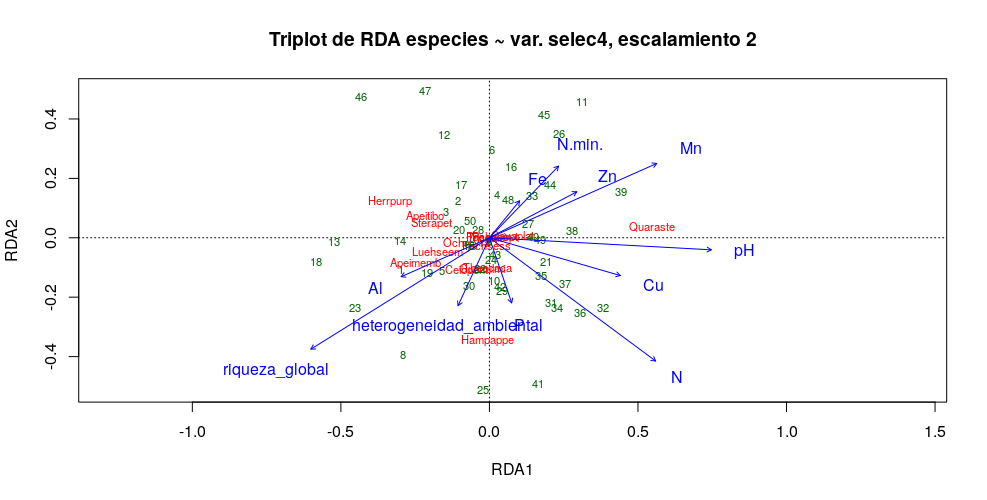
\includegraphics[height=5.00000\textwidth]{triplot_RDA_especies.png}
\caption{Triplot de especies y variables por el método RDA
\label{escalonamiento_triplot}}
\end{figure}

\begin{figure}
\centering
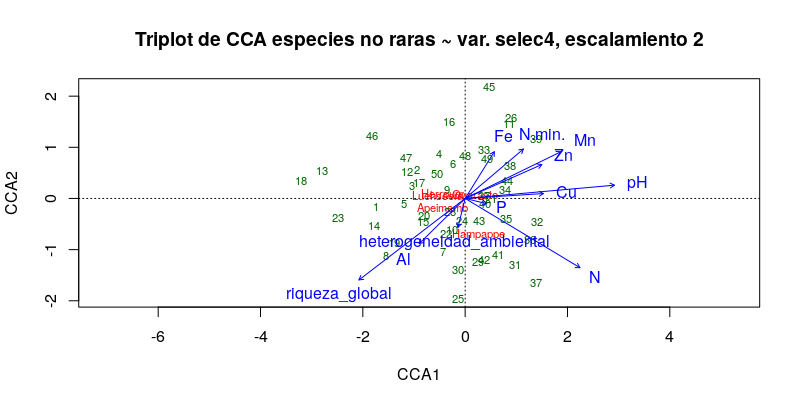
\includegraphics[height=2.00000\textwidth]{Triplot_CCA_varible.png}
\caption{Triplot por el método CCA de especies no raras
\label{escalonamiento_CCA}}
\end{figure}

En el análisis de redundancia (RDA) anterior muestra la colealidad que
existe entre las diferentes variables de especies y elementos del suelo.
Las especies \emph{Hampea appendiculata}, \emph{Ceiba pentandra}, tienen
una gran contribucción en diferentes sitios, que se relacionan con el
Fósforo (P), un poco con el nitrógeno (N), en el caso de \emph{Apeimenb}
tiene mucha asociación con el Aluminio (Al). \emph{Quaraste} es la que
más contribuye al conjunto de sitios con más elementos. Por otro lado,
Fueron excluidas algunas variables por tener el valor \emph{VIF} por
encima de 10 como es el caso del magneso (Mg), calcio(Ca) y las
coordenadas UTM. A pesar de, habían variables con un alto valor
\emph{VIF} por lo que se optó en conservarlas por razones biogeoquimicas
y de asociación (Ver gráfico \ref{escalonamiento_triplot}).

De esta misma manera, en el análisis de correspondencia canónica (CCA)
fueron excluidas las especies con menos de 100 individuos (especies
raras) de la matriz de comunidad, se convervaron 5 en total, y se
excluyeron 11 (Ver gráfico \ref{escalonamiento_CCA}). En ambos gráficos
las variables aparecen en el mismo lugar salvo algunas especies que
desaparecieron en el ``triplot de CCA'' por tener menos de 100
individuos.

\subsection{Análisis de diversidad alpha y
beta}\label{anuxe1lisis-de-diversidad-alpha-y-beta}

Se usaron diferentes métricas para medir los principales componentes de
la diversidad: abundacia y equidad. Se hicieron mediante la equidad de
Shanon (equidad) y antropia de Simpson (abundancia), con los ratios de
Hill, junto con los números de entropía de Renyi y la equidad de Pielu.
En el panel de correlación las especies tuvieron una fuerte asociación
en presencia Magnesio (Mg), calcio (K), zinc (Zn), y una altísima
correlación con el pH sobre todo en la zona de hombrera, perfil de
curvatura media con mayor equidad hacia el Este. Los rojos representan
alta correlación significativa los azules baja (ver figura
\ref{correlacion_geo} y \ref{correlacion_esp}).

En el modelo beta las especies \emph{Hampea appendiculata} y
\emph{Quararibea asterolepis} fueron las más contribuyentes a la
diversidad con 0.18 y 0.14 \% (ver tabla 2),mientras que los sitios con
mayor aportación son el 13 con 0.12 y 46 con 0.86 \% de especies.

En el análisis de rarefacción establece los sitio de mayor y menor
diversidad. En los modelos de abundancia de alpha, el sitio con mayor
riqueza es el 30 con 13 especies y el de menor riqueza es el 45 con 5
especies, la abundancia máxima y mínima fueron en los sitios 6 con 127 y
37 con 31, la abundancia en el sitio más pobre fue 123 en el sitio 45, y
la abundancia en el sitio más rico fue 110 en el sitio 30.

\begin{figure}
\centering
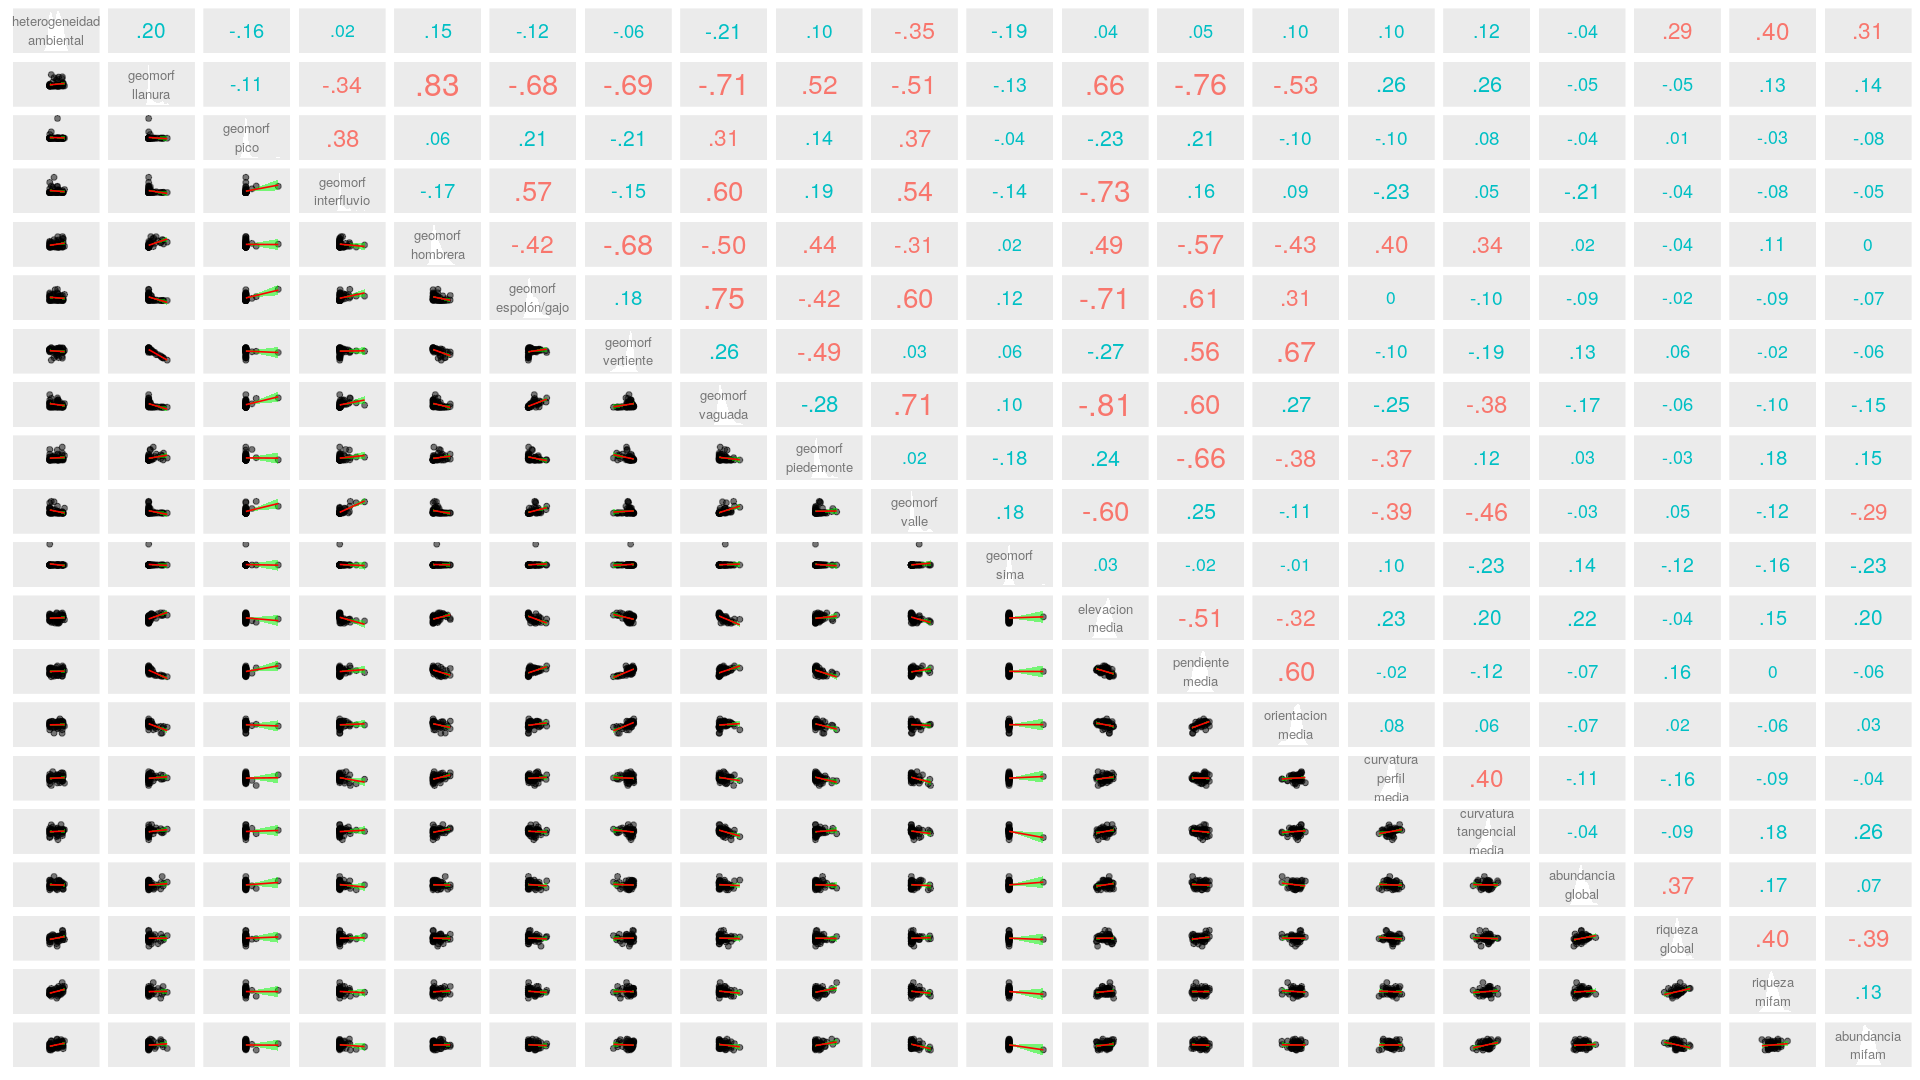
\includegraphics[height=3.00000\textwidth]{matriz_correlacion_geomorf_abun_riq_spearman.png}
\caption{Representación de la distribución de especies por unidad
geomorfológica \label{correlacion_geo}}
\end{figure}

\begin{figure}
\centering
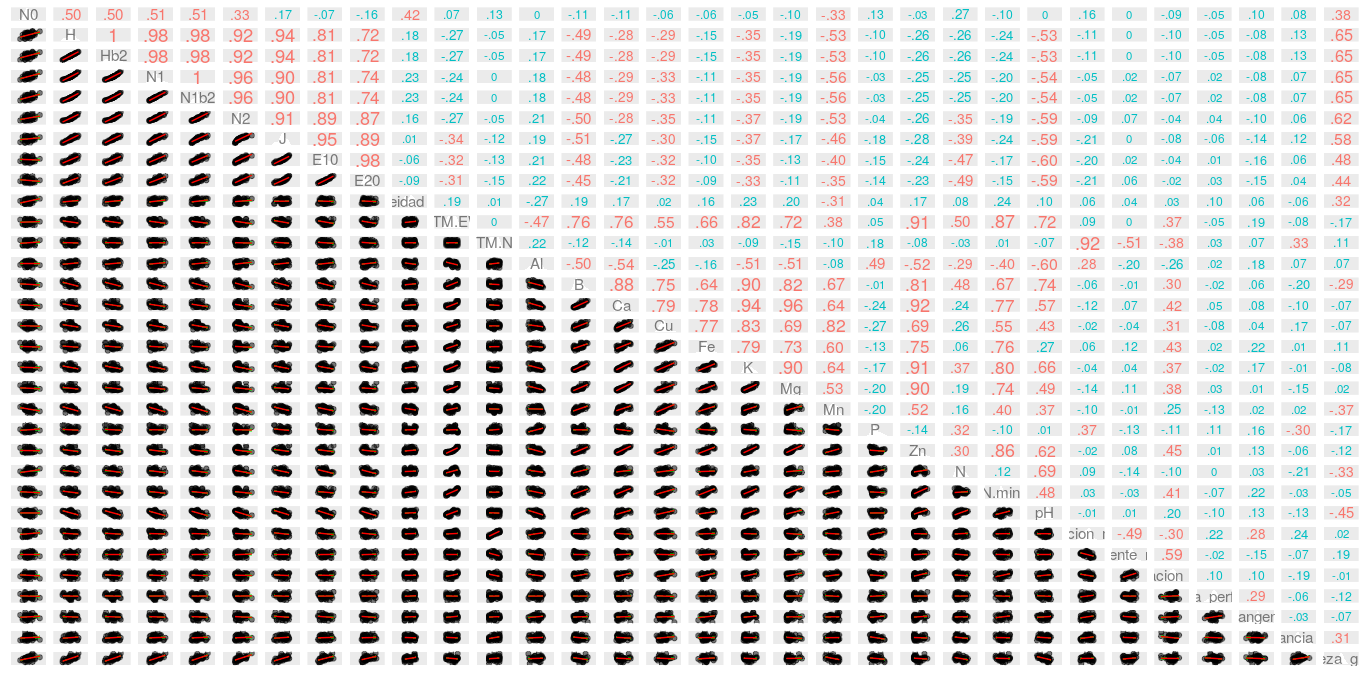
\includegraphics[height=3.00000\textwidth]{Representacion_especies_variables_ambientales.png}
\caption{Representación de especies por variables ambientales
\label{correlacion_esp}}
\end{figure}

{[}Contribución de las especies en la diversidad Beta \label{tabla_2}{]}

\begin{longtable}[]{@{}ll@{}}
\toprule
Especies de planta & valor\tabularnewline
\midrule
\endhead
Apeiba membranacea & 0.08\tabularnewline
Apeiba tibourbou & 0.07\tabularnewline
Hampea appendiculata & 0.14\tabularnewline
Herrania purpurea & 0.11\tabularnewline
Luehea seemannii & 0.09\tabularnewline
Quararibea asterolepis & 0.18\tabularnewline
\bottomrule
\end{longtable}

\subsection{Ecología espacial}\label{ecologuxeda-espacial}

Mediante la pruba de permutación para del \emph{I de Moran} se probó la
autocorrelación entre cada especie de plantas. De acuerdo con el resumen
estadistico las especies con mayor autocorrelación fueron \emph{Apeiba
membranacea}, \emph{Herrania purpurea} y \emph{Quararibea asterolepis}
(ver figura \ref{matriz_esp}). Asimismo, los elementos quimicos del
suelos más represetantivos en la autocorrelación fueron el zinc(Zn) con
0.85\%, el potasio(K) 0.74\%, el calcio (Ca) 0.69 y el pH con 0.72\%. En
cuanto a las zonas geomorfológicas se encuentra una alta correlación en
la llanura, en el espolón, en la vertiente y en la vaguada (ver figura
\ref{matriz_geo}).

\begin{figure}
\centering
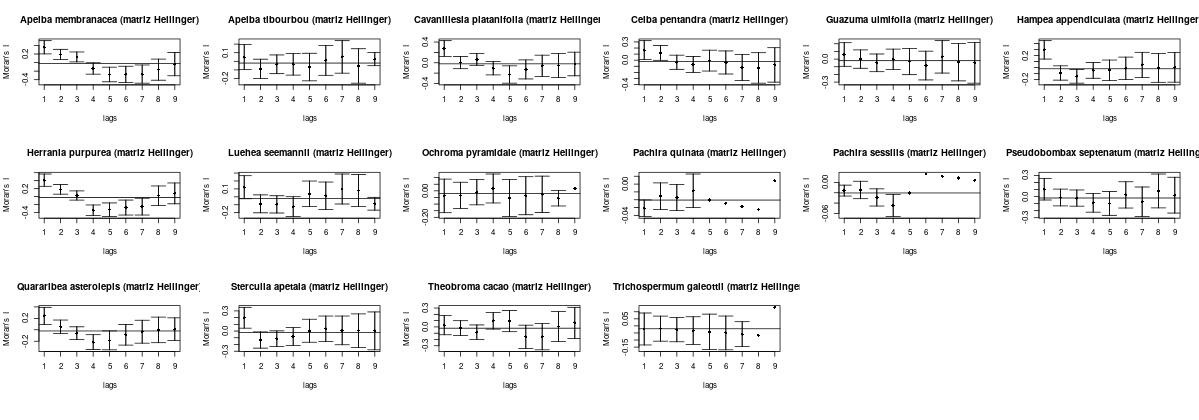
\includegraphics[height=7.00000\textwidth]{correlograma_matriz_de_comunidad_transformada.jpg}
\caption{Correlograma de matriz de comunidad transformada por especies
\label{matriz_esp}}
\end{figure}

\begin{figure}
\centering
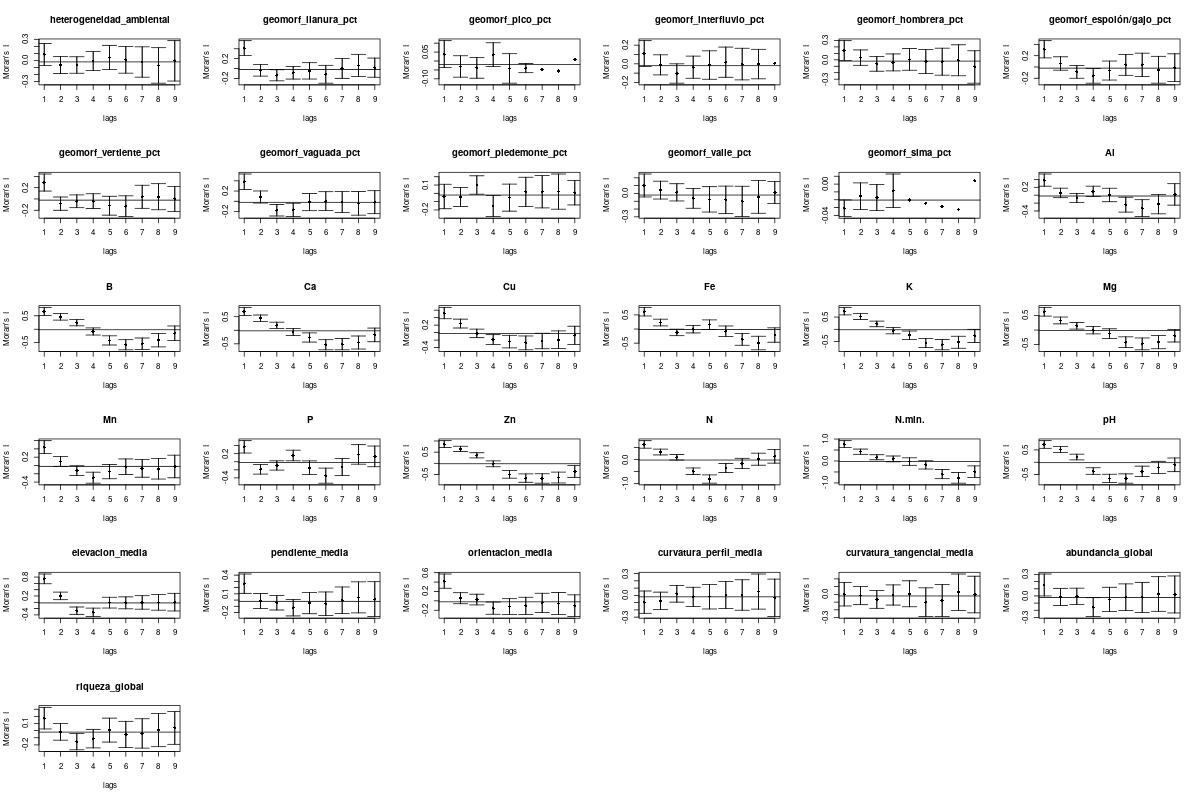
\includegraphics[height=8.00000\textwidth]{correlacion_matriz_comunidad_geomorofologicas_variables_suelo.jpg}
\caption{Correlación entre variables geomorfológicas y elementos del
suelo \label{matriz_geo}}
\end{figure}

\begin{figure}
\centering
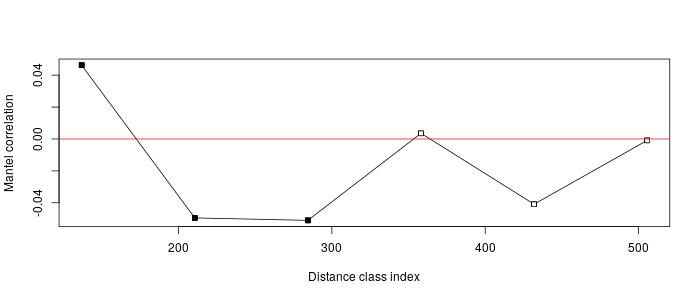
\includegraphics[width=0.90000\textwidth]{mi_fam_correlograma.jpg}
\caption{Correlograma Mantel de las especies de la familia
\label{mantel}}
\end{figure}

El correlograma presenta que para el nivel de significancia 0.04 en los
200 metros existe autocorrelación espacial en la matriz de comunidad.
Esto significa que la posición 1 y 2 son las que se encuentran más
autocorrelacionadas mientras que los otros órdenes (parte de los
residuos) no existe una relación entre especies (Ver figura
\ref{mantel}).

Los clúster LISA mostraron que el pH es el elemento químico con más
autocorrelación espacial, especificamente en la zona de elevación media
de BCI localizada al norte (Ver figura \ref{LISA_ambientales}). En ese
mismo orden, indicó que \emph{Quararibea asterolepis} tiene valores de
grandes de abundancias y autocorrelación seguido de \emph{Sterculia
apetala}, \emph{Theobroma cacao} y \emph{Pseudobombax septenatum} que
presentan un patrón similar (Ver figura \ref{LISA_especies}).Los cuadros
rojos representan la autocorrelación espacial con valores altos y el
azul con valores bajos.

\begin{figure}
\centering
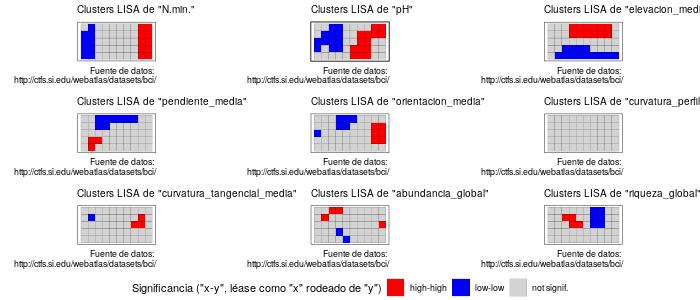
\includegraphics[width=0.90000\textwidth]{cluster_LISA.jpg}
\caption{Clúster LISA aplicado a variables ambientales
\label{LISA_ambientales}}
\end{figure}

\begin{figure}
\centering
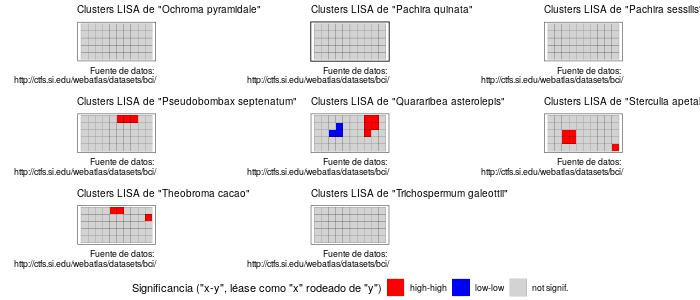
\includegraphics[width=0.90000\textwidth]{cluster_LISA_aplicado_especies_transformadas.jpg}
\caption{Clúster LISA aplicado especies transformadas
\label{LISA_especies}}
\end{figure}

\section{Discusión}\label{discusiuxf3n}

Los resultaron mostraron que familia de plantas \emph{Malvaceae} posee
una abundancia de 3,792 especies agrupadas mayormente en la parte
oriental de manera dispersa en la parcela, con riquezas máximas situadas
en el borde superior central. Esta distribución de especies en grupos
aleatorios depende de diferentes factores abióticos (no vivo) y bióticos
(vivos).

Se determinó que en la mayoria de las especies hay una gran asociación
entre ellas, y desde el punto de vista de la distancia de Jaccard están
muy proximas. Adicionamente, el agrupamiento de especies en forma de
dendograma se generó mediante el método Ward por ser el más facil de
interpretar.

Al analizar por separado los gráficos de escalonamiento de ordenación
RDA y CCA, los resultados indicaron que solo algunos compuestos del
suelo están asociados con especies de la familia, como son el magnesio
(Mg), calcio (Ca) siendo el pH el más representativo del área estudiada.

Se destaca la especie \emph{Quararibea asterolepis} por encima de las
otras de la familia tanto en la diversidad, distribución como en
contribución de los sitios. De igual manera fue la especie con mayor
autocorrelación espacial, seguida de \emph{Apeiba membranacea} y
\emph{Herrania purpurea} las cuales también contribuyeron a la
diversidad de sitios. Las zonas donde se produjo esta autocorrelación
fueron en la llanura, espolón y vertiente en presencia de pH, zinc (Zn),
boro (B) y calcio (Ca). En cambio, las zonas de hombrera y elevación
media presentaron mayor diversidad en presencia de magnesio (Mg), calcio
(Ca), zinc (Zn) que son conocidas por ser zonas húmedas.

La topografía puede verse modificada por los compuestos del suelo en la
vegetación. La cantidad de agua disponible en el suelo, el pH, la
cantidad de nutrientes y la textura del suelo son factores que modifican
la pendiente (relieve) y por lo tanto, influyen en la distribución de
las plantas en los bosques.(Clark, 2002) En BCI en áreas de tierra
firme, el nivel freático puede subir ocasionalmente, y causar periodos
excepcionalmente adversos y hasta letales para la vegetación (Clark,
2002). Por tanto, las condiciones climáticas, factores edáficos y la
topografía del terreno influyen directamente en la distribución y
modificación de las plantas en BCI. En el caso de los compuestos donde
hay escasa correlación puede deberse a un exceso de precipitación o
largos periodos de sequía.

Asimismo, la alta presencia de pH en el suelo genera una acidificación
que provoca una disminución en la disponibilidad de ciertos elementos
nutritivos como son el fósforo, magnesio y calcio en aquellos suelos
donde suelen ser absorbidos por las plantas, por lo tanto una letalidad
más rápida en las plantas.(G.J., 2019).

A partir de los datos estudiados y comparándolos con estudios anteriores
se distingue que las plantas son propensas a desarrollarse en áreas
húmedas y con disponibilidad de agua esto se comprueba por patrones
discontinuo por aglomeración en presencia en las zonas de vaguada, la
llanura, el espolón y la vertiente.

Según investigadores, los patrones de lluvia están cambiando, con
períodos secos extremos más frecuentes en toda la región. En el pasado,
estos períodos secos puedieron haber conducido a un aumento de las tasas
de extinción de fauna y flora y alteración el los compuesto del suelo
(Armuelles, 2021). En este aspecto, si los patrones de lluvias continúan
cambiando con periodos más secos, en dos décadas la Isla Barro Colorado
podría perder especies de plantas como de animales, y esto podrían
ocasionar un aumento de la tasa de extinción de las clases de plantas de
la familia \emph{Malvaceae}.

\section{Agradecimientos}\label{agradecimientos}

Agradezco al profesor de Biogeografía José Ramón Martinez Battle del
área de las ciencias geográficas de la Universidad Autónoma de Santo
Domingo (UASD) por tener la iniciativa, propiciar las investigaciones y
facilitar las herramientas para este estudio.De igual forma a la escuela
de geografía de la UASD por ser fuente de formación de profesionales en
el área de geografía.

De igual forma, al Instituto Smithsonian de Instigaciones Tropicales por
facilitar los datos recogidos de años en la Isla Barro Colorado. Por
último a la estudiante de Ciencias Geográficas Ana Valera por ayudarme a
la redacción de esta investigación.

\section{Información de soporte}\label{informaciuxf3n-de-soporte}

\begin{figure}
\centering
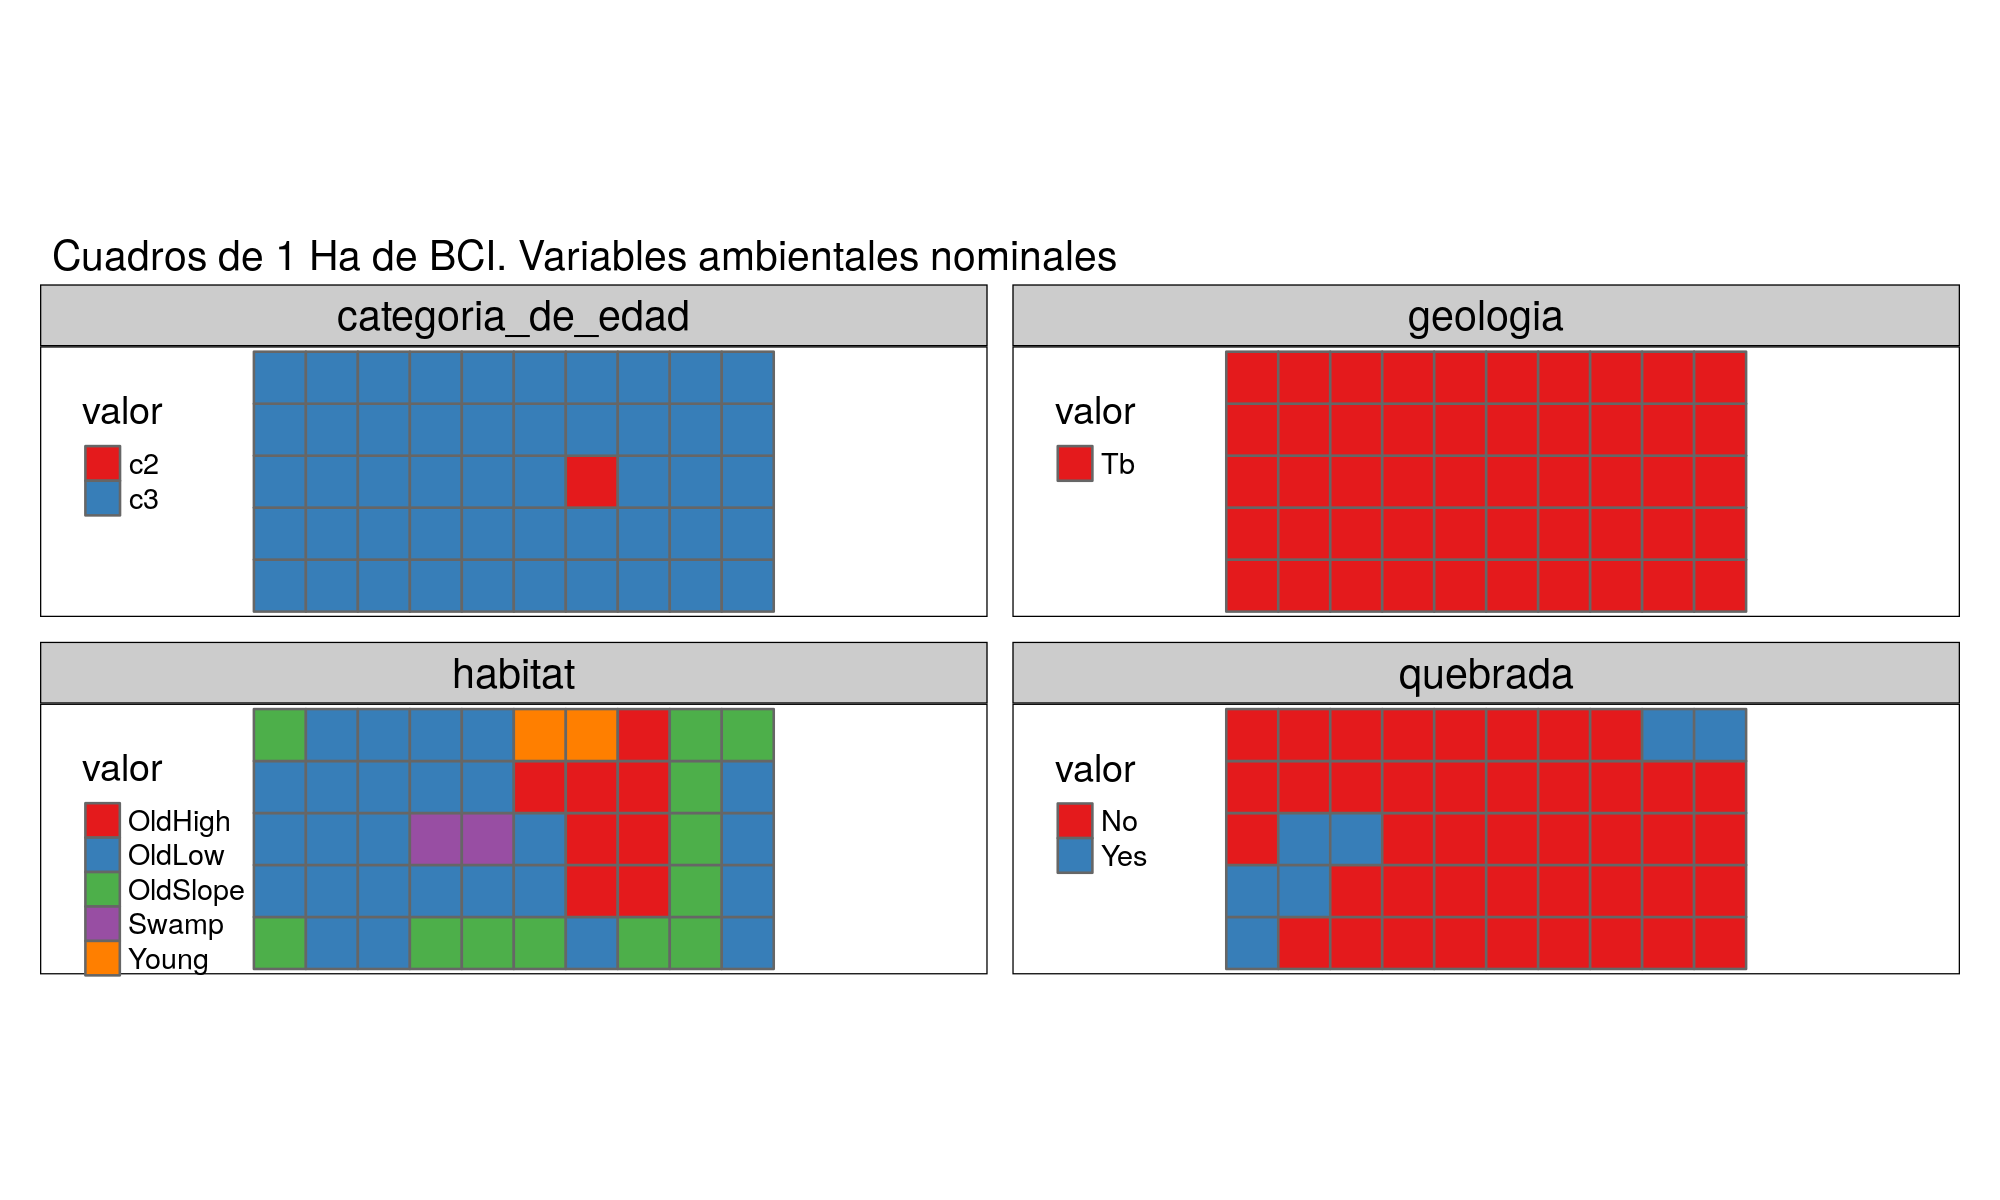
\includegraphics[width=0.70000\textwidth]{mapas_variables_ambientales_nominales_tmap.png}
\caption{Representación de variables ambientales nominales}
\end{figure}

\begin{figure}
\centering
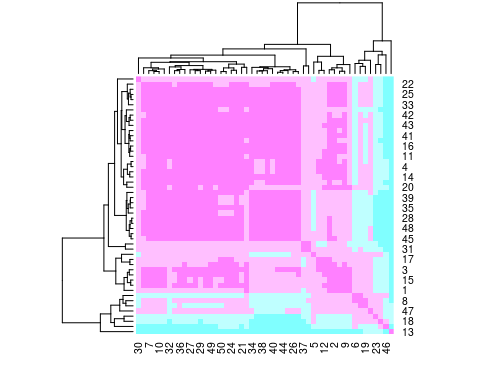
\includegraphics[width=0.60000\textwidth]{mapa_de_calor_ward.png}
\caption{Mapa 4. Matriz anchura de siluetas por el método Ward}
\end{figure}

\begin{figure}
\centering
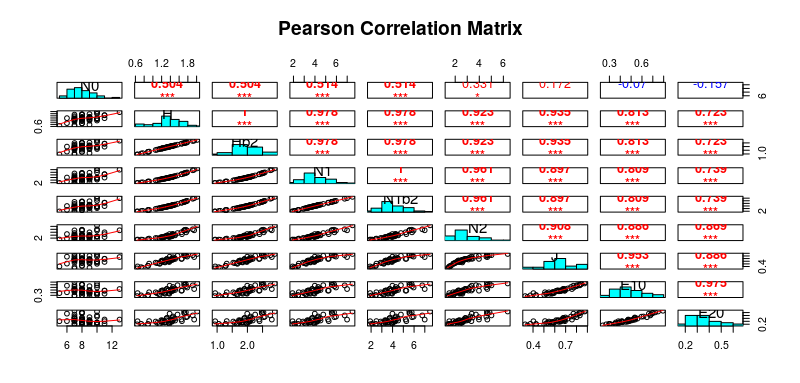
\includegraphics[width=0.70000\textwidth]{Indice_correlacion_Pearson.png}
\caption{Indice de correlación de
pearsons\label{fig:matriz_disimilaridad}}
\end{figure}

\begin{figure}
\centering
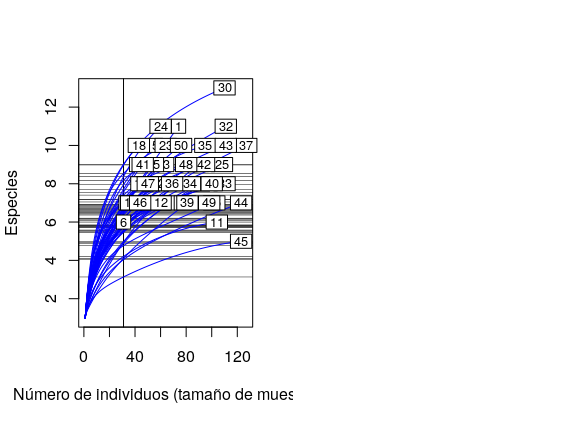
\includegraphics[width=0.80000\textwidth]{grafico_de_rarefaccion.png}
\caption{Gráfico de rarefacción}
\end{figure}

\begin{figure}
\centering
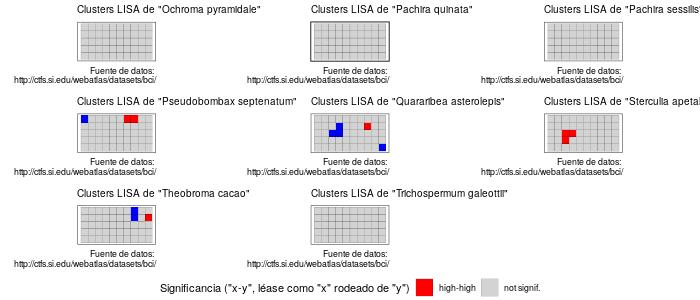
\includegraphics[width=0.70000\textwidth]{cluster_LISA_aplicado_especies_transformadas_sin_tendencia.jpg}
\caption{Cluster LISA aplicado a especies (sin tendencia)}
\end{figure}

\ldots

\section{\texorpdfstring{\emph{Script}
reproducible}{Script reproducible}}\label{script-reproducible}

\subsection{Análisis exploratorio de datos.Riqueza y
abundancia}\label{anuxe1lisis-exploratorio-de-datos.riqueza-y-abundancia}

\begin{verbatim}
#' ---
#' title: "Análisis exploratorio de datos. Riqueza y abundancia"
#' author: "JR"
#' date: "13 de octubre, 2020"
#' output: github_document
#' ---

#' ### Área de cargar paquetes
library(vegan)
library(tidyverse)
library(sf)
source('biodata/funciones.R')

#' ### Área de cargar datos
#' Censo (el objeto se carga con prefijo "censo") y matriz de comunidad (prefijo "mc")
load('biodata/Malvaceae.Rdata')
load('biodata/matriz_ambiental.Rdata') #Matriz ambiental, se carga como "bci_env_grid"

#' ### Imprimir datos en pantalla (impresiones parciales con head)
head(censo_malvc)
head(mc_malvc)
bci_env_grid # No necesita imprimirse parcialmente

#' ### También podemos usar
#' Requiere que se haya cargado ya la colección tidyverse
censo_malvc %>% tibble
mc_malvc %>% tibble

#' ### Lista de especies
sort(colnames(mc_malvc))

#' ### Número de sitios, tanto en matriz de comunidad como en ambiental
#' Verifica que coinciden
nrow(mc_malvc) #En la matriz de comunidad
nrow(bci_env_grid) #En la matriz ambiental

#' ### Riqueza numérica de especies (usando matriz de comunidad) por quadrat
#' Nota: cargar paquete vegan arriba, en el área de paquetes
specnumber(mc_malvc)
sort(specnumber(mc_malvc)) # Ordenados ascendentemente
summary(specnumber(mc_malvc)) # Resumen estadístico

#' ### Abundancia de especies por quadrat
sort(rowSums(mc_malvc))
summary(rowSums(mc_malvc)) # Resumen estadístico

#' ### Abundancia por especie
sort(colSums(mc_malvc))
summary(colSums(mc_malvc)) # Resumen estadístico

#' ### Riqueza numérica de toda la "comunidad"
specnumber(colSums(mc_malvc))

#' ### Abundancia de toda la comunidad
sum(colSums(mc_malvc))

#' ### Una tabla para el manuscrito, es necesario asignarle nombre
#' Para esto, usaré la colección "tidyverse"
abun_sp <- censo_malvc %>%
  group_by(Latin) %>% 
  count() %>% 
  arrange(desc(n))
abun_sp

#' ### Un gráfico para el manuscrito
#' Gráfico de mosaicos de la abundancia por especie por cuadros

abun_sp_<- crear_grafico_mosaico_de_mc(mc_malvc, tam_rotulo = 6)
abun_sp_

\end{verbatim}

\subsection{Análisis exploratorio de datos. Mapas de riqueza y
abundancia global de
Malvaceae}\label{anuxe1lisis-exploratorio-de-datos.-mapas-de-riqueza-y-abundancia-global-de-malvaceae}

\begin{verbatim}
#' ---
#' title: "Análisis exploratorio de datos. Mapas de riqueza y abundancia global y de mi familia"
#' author: "JR"
#' date: "25 de octubre, 2020"
#' output: github_document
#' ---

#' ### Cargar paquetes
library(mapview)
library(tidyverse)
library(vegan)
library(sf)
library(RColorBrewer)

#' ### Cargar datos
load('biodata/matriz_ambiental.Rdata')
load('biodata/Malvaceae.Rdata')

#' ### Explorar el objeto de matriz ambiental
bci_env_grid

#' ### Generar mapa de cuadros sin simbología
mapa_cuadros <- mapView(
  bci_env_grid,
  col.regions = 'grey80',
  alpha.regions = 0.6,
  map.types = 'OpenTopoMap',
  legend = F, zoom = 14,
  zcol = 'id') %>% addStaticLabels() %>%
  leaflet::setView(
    lng = -79.85136,
    lat = 9.15097,
    zoom = 15)
mapa_cuadros
mapa_cuadros %>% mapshot(file = 'mapa_cuadros.png') #Genera archivo

#' ### Paletas
Azul <- colorRampPalette(brewer.pal(8, "Blues"))
rojo <- colorRampPalette(brewer.pal(8, "Reds"))

#' ### Mapa de cuadros, simbología por abundancia global
mapa_cuadros_abun_global <- mapView(
  bci_env_grid,
  layer.name = 'abundancia',
  alpha.regions = 0.6,
  map.types = 'OpenTopoMap',
  legend = T, zoom = 14,
  col.regions = azul,
  zcol = 'abundancia_global') %>%
  addStaticLabels(label = bci_env_grid$abundancia_global, textsize = "7pt") %>%
  leaflet::setView(
    lng = -79.85136,
    lat = 9.15097,
    zoom = 15)
mapa_cuadros_abun_global
mapa_cuadros_abun_global %>% mapshot(file = 'mapa_cuadros_abun_global.png') 

#' ### Mapa de cuadros, simbología por riqueza global
mapa_cuadros_riq_global <- mapView(
  bci_env_grid,
  layer.name = 'riqueza',
  alpha.regions = 0.6,
  map.types = 'OpenTopoMap',
  legend = T, zoom = 14,
  col.regions = rojo,
  zcol = 'riqueza_global') %>%
  addStaticLabels(label = bci_env_grid$riqueza_global, textsize = "7pt") %>%
  leaflet::setView(
    lng = -79.85136,
    lat = 9.15097,
    zoom = 15)
mapa_cuadros_riq_global
mapa_cuadros_riq_global %>% mapshot(file = 'mapa_cuadros_riq_global.png')

#' ### Mapa de cuadros, simbología por abundancia de mi familia
mapa_cuadros_abun_mi_familia <- mapView(
  bci_env_grid %>% mutate(abun = rowSums(mc_malvc)),
  layer.name = 'abundancia',
  alpha.regions = 0.6,
  map.types = 'OpenTopoMap',
  legend = T, zoom = 14,
  col.regions = azul,
  zcol = 'abun') %>%
  addStaticLabels(label = rowSums(mc_malvc)) %>%
  leaflet::setView(
    lng = -79.85136,
    lat = 9.15097,
    zoom = 15)
mapa_cuadros_abun_mi_familia
mapa_cuadros_abun_mi_familia %>% mapshot(file = 'mapa_cuadros_abun_mi_familia.png')
# La mayor abundancia de la familia Malvaceae se concentra en el cluster de la parte oriental, mientras que en la prte occidental los cluster son de baja abundancia.La abundancia global se concentra en la parte occidental, por lo tanto mi familia no sigue el patron que siguen todas las plantas de familia de BIC.


#' ### Mapa de cuadros, simbología por riqueza de mi familia
mapa_cuadros_riq_mi_familia <- mapView(
  bci_env_grid %>% mutate(riq = specnumber(mc_malvc)),
  layer.name = 'riqueza',
  alpha.regions = 0.6,
  map.types = 'OpenTopoMap',
  legend = T, zoom = 14,
  col.regions = rojo,
  zcol = 'riq') %>%
  addStaticLabels(label = specnumber(mc_malvc)) %>%
  leaflet::setView(
    lng = -79.85136,
    lat = 9.15097,
    zoom = 15)
mapa_cuadros_riq_mi_familia
mapa_cuadros_riq_mi_familia %>% mapshot(file = 'mapa_cuadros_riq_mi_familia.png')
#Las riquesas máximas en la familia de plantas Malvaceae se encuentran en el borde superior central, a diferencia de los patrones de riqueza global que se encuentran en el centro y al borde noriental. 
\end{verbatim}

\subsection{Análisis exploratorio de datos. Mapas de variables
ambientales}\label{anuxe1lisis-exploratorio-de-datos.-mapas-de-variables-ambientales}

\begin{verbatim}
#' ---
#' title: "Análisis exploratorio de datos. Mapas de variables ambientales"
#' author: "JR"
#' date: "25 de octubre, 2020"
#' output: github_document
#' ---

#' ### Cargar paquetes
library(mapview)
library(tidyverse)
library(sf)
library(RColorBrewer)

#' ### Cargar datos
load('biodata/matriz_ambiental.Rdata')

#' ### Paletas
azul <- colorRampPalette(brewer.pal(8, "Blues"))
rojo <- colorRampPalette(brewer.pal(8, "Reds"))
rojo_inv <- colorRampPalette(rev(brewer.pal(8, "Reds")))

#' ### Mapa de cuadros, simbología por pendiente
mapa_cuadros_pendiente <- mapView(
  bci_env_grid,
  layer.name = 'pendiente',
  alpha.regions = 0.4,
  map.types = 'OpenTopoMap',
  legend = T, zoom = 14,
  col.regions = rojo,
  zcol = 'pendiente_media') %>%
  addStaticLabels(label = round(bci_env_grid$pendiente_media, 1)) %>%
  leaflet::setView(
    lng = -79.85136,
    lat = 9.15097,
    zoom = 15)
mapa_cuadros_pendiente
mapa_cuadros_pendiente %>% mapshot(file = 'mapa_cuadros_pendiente.png') #Genera archivo

#' ### Mapa de cuadros, simbología por Nitrógeno
mapa_cuadros_nit <- mapView(
  bci_env_grid,
  layer.name = 'N (mg/kg)',
  alpha.regions = 0.4,
  map.types = 'OpenTopoMap',
  legend = T, zoom = 14,
  col.regions = rojo,
  zcol = 'N') %>%
  addStaticLabels(label = round(bci_env_grid$N, 1)) %>%
  leaflet::setView(
    lng = -79.85136,
    lat = 9.15097,
    zoom = 15)
mapa_cuadros_nit
mapa_cuadros_nit %>% mapshot(file = 'mapa_cuadros_nit.png')

#' ### Mapa de cuadros, simbología por pH
mapa_cuadros_ph <- mapView(
  bci_env_grid,
  layer.name = 'pH',
  alpha.regions = 0.4,
  map.types = 'OpenTopoMap',
  legend = T, zoom = 14,
  col.regions = rojo_inv,
  zcol = 'pH') %>%
  addStaticLabels(label = round(bci_env_grid$pH, 1)) %>%
  leaflet::setView(
    lng = -79.85136,
    lat = 9.15097,
    zoom = 15)
mapa_cuadros_ph
mapa_cuadros_ph %>% mapshot(file = 'mapa_cuadros_ph.png')
#'La concentración de PH se encuentra en la parte oriental los porcentaje mas rojos son mas acidos y son los que están en zonas de vaguadas
\end{verbatim}

\subsection{Análisis exploratorio de datos. Correlaciones entre
variables
ambientales}\label{anuxe1lisis-exploratorio-de-datos.-correlaciones-entre-variables-ambientales}

\begin{verbatim}
#' ---
#' title: "Análisis exploratorio de datos. Correlaciones entre variables ambientales"
#' author: "JR"
#' date: "25 de octubre, 2020"
#' output: github_document
#' ---

knitr::opts_chunk$set(fig.width=12, fig.height=8)

#' ### Cargar paquetes
library(tidyverse)
library(sf)
library(ez)
library(psych)
library(vegan)

#' ### Cargar datos
load('biodata/matriz_ambiental.Rdata')
load('biodata/Malvaceae.Rdata')

#' ### Una correlación simple
cor(bci_env_grid$pendiente_media, bci_env_grid$geomorf_vertiente_pct)
plot(bci_env_grid$pendiente_media, bci_env_grid$geomorf_vertiente_pct)
cor.test(bci_env_grid$pendiente_media, bci_env_grid$geomorf_vertiente_pct)

#' ### Generar objeto de columnas numéricas
#' El objeto que generaré, denominado `env_num`, no tendrá las columnas `id` y las de coordenadas UTM, y añadiré la abundancia y riqueza de mi familia. Al mismo tiempo, insertaré un enter (`\n`) en nombres largos de variables, para acomodar los nombres de variables al panel de correlaciones; por ejemplo, el nombre `riqueza_global` se renombra a `riqueza\nglobal`.
env_num <- bci_env_grid %>%
  dplyr::select_if(is.numeric) %>%
  dplyr::select(-id, -matches('^U.*')) %>% 
  st_drop_geometry %>% 
  mutate(
    riqueza_mifam = specnumber(mc_malvc),
    abundancia_mifam = rowSums(mc_malvc)) %>% 
  rename_all(gsub, pattern = '_pct$', replacement = '') %>% 
  rename_all(gsub, pattern = '_| ', replacement = '\n')
env_num %>% tibble

#' ### Panel de correlaciones con herramientas del paquete `graphics` y `psych`
cor(env_num)
ncol(env_num)
pairs(env_num[,sample(1:33, 15)]) # paquete graphics
env_num[,sample(1:33, 15)] %>% pairs.panels #paquete psych

#' ### Panel de correlaciones con `ez`
#' 
#' #### Todas las variables (se empasta). Comentado, sólo mostrado para fines didácticos
# p_cor_todos <- env_num %>%
#   ezCor(r_size_lims = c(4,8), label_size = 4)
# p_cor_todos

#' #### Sólo suelo (elementos y pH), abundancia/riqueza
p_cor_suelo_ar <- env_num %>%
  dplyr::select(matches('^[A-T,Z]|abundancia|riqueza|^pH$', ignore.case = F)) %>%
  ezCor(r_size_lims = c(4,8), label_size = 3)
p_cor_suelo_ar

#' #### Sólo heterogeneidad, geomorfologia, abundancia/riqueza
p_cor_geomorf_ar <- env_num %>%
  dplyr::select(-matches('^[A-T,Z]|pH', ignore.case = F)) %>%
  ezCor(r_size_lims = c(4,8), label_size = 3)
p_cor_geomorf_ar

#' #### Matriz de comunidad
p_cor_mc <- mc_malvc %>%
  rename_all(gsub, pattern = '_| ', replacement = '\n') %>% 
  ezCor(r_size_lims = c(4,8), label_size = 3)
p_cor_mc
\end{verbatim}

\subsection{Análisis exploratorio de datos. Mapas de variables
ambientales por
lotes}\label{anuxe1lisis-exploratorio-de-datos.-mapas-de-variables-ambientales-por-lotes}

\begin{verbatim}
#' ---
#' title: "Análisis exploratorio de datos. Mapas de variables ambientales por lotes"
#' author: "JR"
#' date: "3 de diciembre, 2020"
#' output: github_document
#' ---

knitr::opts_chunk$set(fig.width=12, fig.height=8)

#' ## Preámbulo
#' 
#' ### Cargar paquetes
#' 
library(tmap)
library(sf)
library(tidyverse)
library(RColorBrewer)
#' 
#' ### Cargar datos
#' 
load('biodata/matriz_ambiental.Rdata')
#' 
#' ## Convertir a KML
#' 
st_write(
  bci_env_grid %>% rename(Name = id),
  driver = 'KML',
  dsn = 'matriz_ambiental.kml')
st_write(
  bci_env_grid %>% rename(Name = id) %>% st_centroid(),
  driver = 'KML',
  dsn = 'matriz_ambiental_puntos.kml')
#' 
#' Uní los dos archivos anteriores en un único KML nombrado como `mapa_cuadros_1ha_para_google_earth.kml`, el cual muestra los puntos como rótulos identificadores de cada cuadro de 1 Ha dentro de sus correspondientes polígonos. Visualizar dicho archivo en GoogleEarth para un "recorrido virtual" por BCI.
#' 
#' ## Generar mapas por lotes
#' 
#' ### Variables ambientales numéricas con `ggplot2`
#' 
mapas_var_amb_num_gg <- bci_env_grid %>%
  select_if(is.numeric) %>% 
  gather(variable, valor, -geometry) %>% 
  group_by(variable) %>% 
  mutate(
    valor = scales::rescale(valor, to = c(0, 1)),
    id = rep(1:50)) %>% 
  ggplot +
  aes(geometry = geometry, fill = valor) +
  theme(axis.text = element_blank()) +
  geom_sf(lwd = 0.1, color = 'grey50', alpha = 0.8) + coord_sf() +
  scale_fill_gradientn(colours = brewer.pal(11, 'BrBG')) +
  geom_sf_text(aes(label = id, color = between(valor, 0.3, 0.7)), size = 1.75) +
  scale_color_manual(guide = FALSE, values = c("white", "black")) +
  facet_wrap(~ variable, ncol = 6) + 
  ggtitle('Cuadros de 1 Ha de BCI. Variables ambientales numéricas escaladas de 0 a 1')
mapas_var_amb_num_gg
#'
#' PNG
#'
png(
  filename = 'mapas_variables_ambientales_numericas.png',
  width = 1700, height = 1080, res = 150)
mapas_var_amb_num_gg
dev.off()
#' 
#' ### Variables ambientales numéricas con `tmap`
#' 
mapas_var_amb_num_tmap <- bci_env_grid %>%
  select_if(is.numeric) %>% 
  gather(variable, valor, -geometry) %>% 
  group_by(variable) %>% 
  mutate(
    valor = scales::rescale(valor, to = c(0, 1)),
    id = rep(1:50)) %>% 
  tm_shape() +
  tm_polygons(col = 'valor',
              palette = brewer.pal(11, 'BrBG'),
              style ='cont',
              legend.is.portrait = FALSE) +
  tm_facets(by = 'variable', ncol = 6, nrow = 6) +
  tm_layout(main.title="Cuadros de 1 Ha de BCI. Variables ambientales numéricas escaladas de 0 a 1",
            main.title.size = 0.7,
            legend.outside.position="bottom",
            legend.outside=TRUE,
            legend.width = 0.2,
            legend.text.size = 0.5,
            legend.stack="horizontal", 
            outer.margins=0)
mapas_var_amb_num_tmap
#'
#' PNG
#' 
png(
  filename = 'mapas_variables_ambientales_numericas_tmap.png',
  width = 1800, height = 1400, res = 350, pointsize = 12)
mapas_var_amb_num_tmap
dev.off()
#' 
#' ### Variables ambientales nominales con `tmap`
#' 
mapas_var_amb_nom_tmap <- bci_env_grid %>%
  select_if(negate(is.numeric)) %>% 
  gather(variable, valor, -geometry) %>% 
  tm_shape() +
  tm_polygons(col = 'valor',
              palette = brewer.pal(8, 'Set1'),
              legend.show = T) +
  tm_facets(by = 'variable', ncol = 2, free.scales = T, free.coords = T) +
  tm_layout(main.title="Cuadros de 1 Ha de BCI. Variables ambientales nominales",
            main.title.size = 0.7,
            asp = 3.5,
            legend.text.size = 0.7)
mapas_var_amb_nom_tmap
#'
#' PNG
#' 
png(
  filename = 'mapas_variables_ambientales_nominales_tmap.png',
  width = 2000, height = 1200, res = 350, pointsize = 12)
mapas_var_amb_nom_tmap
dev.off()
\end{verbatim}

\subsection{Medición de asociación. Introducción a los modos de análisis
Q y R. Modo Q aplicado a la paradoja de
Orlóci}\label{mediciuxf3n-de-asociaciuxf3n.-introducciuxf3n-a-los-modos-de-anuxe1lisis-q-y-r.-modo-q-aplicado-a-la-paradoja-de-orluxf3ci}

\begin{verbatim}
#' ---
#' title: "Medición de asociación. Introducción a los modos de análisis Q y R. Modo Q aplicado a la paradoja de Orlóci"
#' author: "JR"
#' date: "3 de noviembre, 2020"
#' output: github_document
#' ---
#'
knitr::opts_chunk$set(fig.width=8, fig.height=5)
#'
#'  ## Preámbulo
#'  
#' ### Cargar paquetes
library(vegan)
library(adespatial)
library(tidyverse)
library(gridExtra)
source('biodata/funciones.R')
#' 
#' ## Modos Q y R
#' 
#' En modo Q mides asociación entre pares de objetos, como por ejemplo, entre dos sitios de muestreo. En este modo, mides la asociación por medio de **la disimilaridad y la similaridad** entre pares de objetos, usando métricas como la **distancia euclídea o la similaridad de Jaccard**.
#' 
#' En modo R mides asociación entre pares de descriptores, como por ejemplo, entre dos variables, o dos especies. En este caso mides la asociación por medio de **la dependencia entre variables**, usando por ejemplo la **covarianza o el índice de correlación**.
#' 
#' ## Modo Q: matrices de disimilaridad entre objetos
#' 
#' ### Modo Q para datos cuantitativos de especies (abundancia). La paradoja de Orlóci
#' 
#' La paradoja de Orlóci (1978) plantea que la distancia euclidea es más pequeña entre dos sitios que no comparten especies que entre sitios que sí las comparten.
#' 
#' Esta paradoja se explica por la presencia de "ceros" (especies ausentes) en la matriz de comunidad, los cuales contribuyen a aumentar la similaridad de forma ficticia. Esto se comprueba de manera directa en la matriz de disimilaridad (=distancia). __La matriz de disimilaridad es simplemente una matriz de distancia__. La disimilaridad (D) también la puedes obtener a partir de la similaridad (S), aplicando la fórmula D = 1 - S, y viceversa, S = 1 - D.
#'
#' Te muestro la paradoja con un ejemplo y, posteriormente, te explico cómo solucionar el problema de los ceros. Sea una matriz de comunidad `mc_orloci` de 2 especies y tres sitios...
#' 
(mc_orloci <- tibble(
  sp1 = c(1, 0, 4),
  sp2 = c(1, 0, 8),
  sitio = paste0('sit', 1:3)) %>% 
    column_to_rownames('sitio'))
#' 
#' ...donde ambas especies están ausentes en `sit2`, en `sit1` presentes con poca abundancia y en `sit3` con valores relativamente extremos.
#' 
#' En modo Q, calcularé la "distancia" o "disimilaridad" entre sitios según las especies que los caracterizan. En el lenguaje R, es común usar la función `dist` para calcular la matriz de distancias, pero en ecología se usa también `dist.ldc` del paquete `adespatial`. Las matrices de distancia normalmente se muestran de la siguiente manera (por defecto, sólo el triángulo inferior):
#' 
(dist.ldc(mc_orloci, "euclidean", silent = T))
#' 
#' Te muestro un gráfico de dispersión de los sitios según la abundancia de especies (los ejes representan la abundancia de cada especie). Puedes comprobar que la distancia entre `sit1` y `sit2` es pequeña, mientras que entre `sit1` y `sit3` es grande.
#' 
mc_orloci %>% rownames_to_column('id') %>% 
  ggplot() +
  aes(x = sp1, y = sp2, label = id) +
  geom_point(size = 3) +
  geom_text(vjust="inward",hjust="inward", size = 5, color = 'grey40') +
  coord_equal() +
  theme_bw() +
  theme(text = element_text(size = 16))
#'
#' Para facilitar la lectura de las distancias, en esta explicación ordeneré las matrices de distancia en columnas, usando la función de ayuda `organizar_matriz_distancia`. La primera que generaré es la de distancias euclideas a partir de datos brutos:
#' 
(d_euc <- dist.ldc(mc_orloci, "euclidean", silent = T) %>%
    organizar_matriz_distancia(func_dist = 'Euclidean'))
#' 
#' Siendo los sitios 1 y 2 tan diferentes en cuanto a las especies que los componen (de hecho, no comparten especies), ¿por qué están tan próximos? Asimismo, los sitios 1 y 3 comparten especies, entonces, ¿por qué están tan distantes (=disímiles)? La explicación se atribuye a los ceros y a los valores de abundancia extremos. El hecho de que un par de sitios registren varias ausencias (o pseudo-ausencias), hace que "aparezcan" muy próximos (similares) en el espacio euclídeo. Esta paradoja sugiere que es necesario evitar la distancia euclídea a partir de datos brutos como métrica para comparar sitios.
#' 
#' Existen distintas maneras de solucionar el problema planteado en la paradoja, normalmente recurriendo a métodos de estandarización de las abundancia brutas, y luego calculando distancia euclídea. Es decir, se obtiene una matriz de comunidad transformada y, a partir de ella, se obtienen distancias. Los métodos de transformación más comunes son el de cuerdas (*chord*), *ji*-cuadrado y *Hellinger*. La función `dist.ldc` del paquete `adespatial` provee una solución en un único paso para cada caso (transformar + calcular distancias).
#' 
#' - *Chord*:
#' 
d_cho <- dist.ldc(mc_orloci, "chord", silent = T) %>%
  organizar_matriz_distancia(func_dist = 'Chord')
#' 
#' - *Ji*-cuadrado:
#' 
d_chi <- dist.ldc(mc_orloci, "chisquare", silent = T) %>%
  organizar_matriz_distancia(func_dist = 'chi-square distance')
#' 
#' - *Hellinger* (valores primero divididos por abundancia total > sqrt)
#' 
d_hel <- dist.ldc(mc_orloci, "hellinger", silent = T) %>%
  organizar_matriz_distancia(func_dist = 'Hellinger')
#' 
#' - Uniendo y comparando
(d_todas <- bind_rows(d_euc, d_cho, d_chi, d_hel))
#' 
#' Verás que el par `sit1|sit3` tiene corta distancia, es decir, son muy parecidos (0.17 en *Hellinger*, e igualmente, corta distancia relativa en *ji*-cuadrado y en *chord*). Esto se debe a la transformación, basada en estandarización. Es lógico que este par sea muy similar, puesto que comparten las únicas dos especies de la comunidad. Por lo tanto, las tres transformaciones empleadas corrigen el problema planteado en la paradoja de Orlóci.
#' 
#' Nota igualmente que, tanto los pares `sit1`|`sit2` y `sit2|sit3` están distantes (distancia 1), lo cual también es deseable. Por tal razón, snos interesa explorar las matrices de comunidad original y la transformada. La función `dist.ldc` realiza dos pasos: primero genera una matriz de comunidad transformada y luego calcula la distancia. Para replicar el proceso que realiza `dist.ldc`, es necesario generar primero la matriz transformada y luego pasar directamente a calcular distancia. Repasa primero la matriz de comunidad original:
#' 
mc_orloci
#' 
#' A continuación, generaré la matriz transformada según el método *chord*. Esta matriz se calcula obteniendo primero el cuadrado de cada valor de abundancia y luego dividiéndolo (estandarizando) por la suma de los cuadrados de toda la fila o sitio (vector unitario). El resultado final, es decir, la matriz con valores transformados, se obtiene a partir de la raíz cuadrada de cada valor.
#' 
mc_orloci_norm <- sqrt(mc_orloci^2/rowSums(mc_orloci^2)) %>%
  replace(is.na(.), 0)
mc_orloci_norm
#' 
#' La matriz de comunidad se dice que está "normalizada". Lo anterior se puede hacer más fácilmente con `decostand` de `vegan` (resultado idéntico):
#' 
(mc_orloci_norm <- decostand(mc_orloci, "normalize"))
#' 
#' Al graficar los sitios sobre un espacio bidimensional, cada eje representando una especie, se obtienen resultados diferentes a los que se obtuvieron con la matriz original:
#' 
p1 <- mc_orloci %>%
  rownames_to_column('id') %>% 
  ggplot() +
  aes(x = sp1, y = sp2, label = id) +
  geom_point(size = 3) +
  geom_text(vjust="inward",hjust="inward", size = 5, color = 'grey40') +
  coord_equal() +
  theme_bw() +
  theme(text = element_text(size = 16)) +
  ggtitle('mc original')
p2 <- mc_orloci_norm %>%
  rownames_to_column('id') %>% 
  ggplot() +
  aes(x = sp1, y = sp2, label = id) +
  geom_point(size = 3) +
  geom_text(vjust="inward",hjust="inward", size = 5, color = 'grey40') +
  coord_equal() +
  theme_bw() +
  theme(text = element_text(size = 16)) +
  ggtitle('mc transformada')
grid.arrange(p1, p2, nrow = 1)
#'   
#' - Por último, para completar el proceso realizado por `dist.ldc`, debes calcular la distancia euclidea a partir de esta matriz. Verás que obtienes el mismo resultado que con la función `dist.ldc`:
#' 
(d_cho_2_pasos <- dist(mc_orloci_norm, method = 'euclidean')) %>% 
  organizar_matriz_distancia(func_dist = 'Chord en dos pasos')
#'
#'  Compara la matriz anterior con la generada por `dist.ldc`, objeto `d_cho`:
d_cho
\end{verbatim}

\subsection{Edición de asociación. Modo Q aplicado a mi familia
asignada}\label{ediciuxf3n-de-asociaciuxf3n.-modo-q-aplicado-a-mi-familia-asignada}

\begin{verbatim}
#' ---
#' title: "Medición de asociación. Modo Q aplicado a mi familia asignada"
#' author: "JR"
#' date: "9 de noviembre, 2020"
#' output: github_document
#' ---

knitr::opts_chunk$set(fig.width=12, fig.height=8)

#' ## Preámbulo

#' ### Cargar paquetes
library(vegan)
library(adespatial)
library(broom)
library(tidyverse)
library(sf)
library(cluster)
library(gclus)
source('biodata/funciones.R')

#' ### Cargar datos
#' 
load('biodata/matriz_ambiental.Rdata')
load('biodata/Malvaceae.Rdata')
#' 
#' ## Modo Q: matrices de disimilaridad entre objetos
#' 
#' ### Modo Q para datos cuantitativos de especies (abundancia). Datos de mi familia asignada
#' 
#' Aplicado a mi familia asignada de BCI, en la forma de matriz de distancia euclídea, utilizando la transformación *Hellinger*:
#' 
mi_fam_d_hel <- dist.ldc(mc_malvc, "hellinger", silent = T)
mi_fam_d_hel %>% tidy # Para evitar desbordar la consola
#' 
#' Para interpretar esta matriz, es necesario representarla gráficamente. En la representación elegida a continuación, color fucsia (magenta, rosa) significa "corta distancia=muy similares", y cian (celeste) significa "gran distancia=poco similares":
#' 
coldiss(mi_fam_d_hel, diag = T)
#' 
#' Mejorable el gráfico, quizá este es más explícito:
#' 
coldissgg(mi_fam_d_hel, ordered = T, nc = 4, fsz = 0)
#' 
#' Con valores de distancia sobreimpresos (se empastan un poco)
#' 
coldissgg(mi_fam_d_hel, ordered = T, nc = 4, fsz = 1.5)
#' 
#' Puedes guardar el gráfico usando el botón `Export` de la pestaña `Plots`
#' 
#' Una forma alterna de guardar el gráfico es mediante funciones de R. La calidad de gráficos exigida en revistas, suele requerir usar dichas funciones específicas, porque permiten más control. A continuación uso una de ellas, la función `png`, con la cual "abro un dispositivo gráfico. Luego, imprimo el gráfico que deseo guardar y finalmente cierro el dispositivo mediante `dev.off` Por ejemplo:
#' 
png(
  filename = 'matriz_disimilaridad_hellinger.png',
  width = 2400, height = 1200, pointsize = 32
)
coldiss(mi_fam_d_hel, diag = T)
dev.off()
#' 
#' MUY IMPORTANTE. La última función, `dev.off()`, es necesaria para cerrar el dispositivo. Si no la ejecutas, no se generarán gráficos en el dispositivo estándar (e.g. pestaña `Plots`)
#' 
#' ### Modo Q para datos binarios (presencia/ausencia)
#' 
#' Habitualmente, sólo dispones de datos de presencia/ausencia. En tales casos, existe un conjunto de herramientas basadas en métricas de disimilaridad o de similaridad, con las que podrás analizar patrones de asociación. En la bibliografía, encontrarás muchos ejemplos de las métricas (de disimilaridad o similaridad) de Jaccard o de Sorensen (esta última equivalente a "Bray-Curtis").
#' 
#' Un error común consiste en referirse a los índices de Jaccard y de Sorensen "a secas", sin especificar si se trata de disimilaridad (distancia) o de similaridad. Toda métrica de disimilaridad tiene un complemento a 1 que la convierte en métrica de similaridad, y viceversa; por lo tanto, se trata de mediciones claramente opuestas. Cuando el/la autor/a no declara qué está midiendo, la interpretación podría resultar ambigua e incluso contradictoria. Por esta razón, es necesario especificar si se trata de un índice de disimilaridad o de similaridad.
#' 
#' Si alguna vez te enfrentas a textos donde no se especifica qué tipo de métrica se usa, te sugiero preguntarte ¿qué mide este índice? Si comparas varios sitios por pares, y notas que a mayor valor del índice en cuestión observas mayor similitud o parecido entre los sitios (e.g. mayor proporción de especies compartidas), entonces se trata de un índice de similaridad. Si por el contrario, a mayor valor se evidencia mayor disimilitud o diferencia entre pares de sitios (e.g. mayor proporción de especies NO compartidas), entonces se trata de un índice de distancia o disimilaridad.
#' 
#' Recalco: **es imprescindible declarar qué tipo de métrica estás usando**. Ejemplos de redacción:
#' 
#' - Correcto: "índice de **disimilaridad** de Jaccard", "índice de **similaridad** de Sorensen", o simplemente "**similaridad** de Jaccard", "**distancia** de Jaccard".
#' 
#' - Incorrecto: "índice de Jaccard", "índice de Sorensen".
#' 
#' A continuación, muestro cómo calcular la **distancia de Jaccard** (**D<sub>J</sub>**) en un único paso usando la función `vegdist`.
#' 
mi_fam_jac <- vegdist(mc_malvc, method = 'jac', binary = T)
mi_fam_jac %>% tidy # Mostrando sólo las primeras 10 combinaciones en modo data.frame
#' 
#' El argumento `binary=T` en `vegdist` "ordena" que se realice primero `decostand(mc_apcyn_melic_saptc, method = 'pa')`, lo cual convierte la matriz de comunidad en una de presencia/ausencia, con la que posteriormente se calculará la matriz de distancia.
#' 
#' En esta matriz de disimilaridad, al igual que en la anterior, un valor pequeño (rosa) significa que los sitios comparados son muy parecidos. Por ejemplo, en el gráfico no ordenado (izquierda), verás que, por ejemplo, los sitios 1 y 2, y los sitios 3 y 4 son muy similares; en el gráfico ordenado por valor de distancia (derecha), notarás por ejemplo que 35 y 19 son muy similares.
#'  
coldiss(mi_fam_jac, diag = T)
#' 
#' La distancia de Jaccard (**D<sub>J</sub>**) se puede expresar como "la proporción de especies no compartidas". En este caso, para la comparación entre los sitios 1 y 2, dicho valor es de 8.33%, que equivale a decir "hay sólo un 8.33% de exclusividad" (por lo tanto, hay mucha similaridad). Si se tratara de la similaridad de Jaccard (**S<sub>J</sub>**) obtendríamos el complemento a 1, que equivale de hecho a "la proporción de especies compartidas", es decir, 91.67%.
#' 
#' Como la distancia de Jaccard (**D<sub>J</sub>**) es el complemento a 1 de la similaridad de Jaccard (**S<sub>J</sub>**), es decir, **D<sub>J</sub>=1-S<sub>J</sub>**, y dado que arriba calculamos la distancia, para obtener la similaridad, sólo hay que restarle el valor de distancia a 1 (**S<sub>J</sub>=1-D<sub>J</sub>**).
#' 
(1 - mi_fam_jac) %>% tidy %>% rename(similaridad=distance) #Similaridad
#'
#' Dado que este resultado muestra la similaridad, podemos leerlo como "el sitio 1 y el 2 comparten un 91.67% de sus especies".
#' 
#' La fórmula de la similaridad de Jaccard es **S<sub>J</sub>=a/(a+b+c)**, donde **a** es el número de especies compartidas (presentes en ambos sitios comparados), **b** el número de especies exclusivas del sitio 2, y **c** el número de especies exclusivas del sitio 1.
#' 
#' Para obtener las variables **a**, **b** y **c**, usaré La función `betadiver` del paquete `vegan`:
#' 
mi_fam_abc <- betadiver(mc_malvc) 
mi_fam_abc %>%
  map(tidy) %>%
  map(slice, 1) %>%
  map_df(I, .id = 'tipo') %>% 
  dplyr::select(tipo, n_especies=distance)
#' 
#' Puedes notar que ambos sitios comparten 11 especies (**a**), que el sitio 2 no tiene especies exclusivas (**b**) y que el sitio 1 tiene 1 especie exclusiva (**c**). Es decir, de 12 especies en total en ambos sitios, hay 11 compartidas, por lo tanto:
#' 
round(11/12*100,2) #Porcentaje de especies compartidas = similaridad
#' 
#' Con `betadiver` también puedes calcular índices de similaridad. Por ejemplo, el Jaccard se calcula así:
#' 
betadiver(mc_malvc, method = 'j') %>% tidy
#' 
#' No obstante, usaremos esta función en los análisis de diversidad beta más adelante.
#' 
#' Además de la distancia de Jaccard, otra distancia muy utilizada es la de Sorensen o Bray-Curtis. Se calcula fácilmente con la función `vegdist`:
#' 
mi_fam_sor <- vegdist(mc_malvc, method = 'bray', binary = T)
mi_fam_sor %>% tidy
coldiss(mi_fam_sor, diag = T)
#' 
#' ### Modo Q para datos cuantitativos, NO de abundancia de especies (variables ambientales)
#' 
#' En este ejemplo, usaré sólo variables de suelo, todas cuantitativas, puedes combinar con otras variables que hayas detectado como relevantes en el análisis de correlación. Nota que convertiré cada variable en puntuaciones *z* mediante la función `scale`. Dado que cada variable tiene su propia escala de medición, si se compararan sin transformación, se obtendrían resultados inconsistentes.
#' 
env_suelo_punt_z <- bci_env_grid %>%
  st_drop_geometry() %>% 
  dplyr::select(matches('^[A-T,Z]|^pH$', ignore.case = F)) %>% 
  scale()
env_suelo_punt_z_d <- dist(env_suelo_punt_z)
env_suelo_punt_z_d %>% tidy
coldiss(env_suelo_punt_z_d, diag = T)
#'
#' ### Modo Q para datos cualitativos y cuantitativos (mixtos), NO de abundancia de especies (variables ambientales)
#' 
#' En este ejemplo, usaré las siguientes variables mixtas (funciona igualmente para datos cualitativos solamente):
#' 
#' - `hetereogeneidad_ambiental`. Índice cuantitativo calculado como la diversidad de Simpson a partir de frecuencias de tipos de micro-hábitats.
#' 
#' - `habitat`. Tipo de hábitat. Asume los siguientes valores posibles: *OldHigh*, *OldLow* y *OldSlope* (bosque viejo en relieve alto, en vertientes y relieve bajo, respectivamente), *Swamp* (bosque en área encharcable) *Young* (bosque joven).
#' 
#' - `quebrada`. Informa sobre si hay o no quebrada. Los valores posibles son *Yes* o *No*.
#' 
env_mix <- bci_env_grid %>%
  st_drop_geometry() %>%
  dplyr::select(heterogeneidad_ambiental, habitat, quebrada)
env_mix_d <- daisy(x = env_mix, metric = 'gower')
env_mix_d %>% as.dist %>% tidy
env_mix_d %>% coldiss(diag = T)
\end{verbatim}

\subsection{Edición de asociación. Modo R aplicado a mi familia
asignada}\label{ediciuxf3n-de-asociaciuxf3n.-modo-r-aplicado-a-mi-familia-asignada}

\begin{verbatim}
r paste (readLines('ma_3:Medicion_de_asociación.R'), collapse = '\n')
\end{verbatim}

\subsection{Análisis de agrupamiento (cluster analysis). Parte 2:
Interpretación y comparación de
resultados}\label{anuxe1lisis-de-agrupamiento-cluster-analysis.-parte-2-interpretaciuxf3n-y-comparaciuxf3n-de-resultados}

\begin{verbatim}
#' ---
#' title: "Análisis de agrupamiento (cluster analysis). <br> Parte 2: Interpretación y comparación de resultados"
#' author: "JR"
#' date: "11 de noviembre, 2020"
#' output: github_document
#' ---

knitr::opts_chunk$set(fig.width=12, fig.height=8)

#' ## Preámbulo
#' 
#' ### Cargar paquetes
#' 
library(vegan)
library(tidyverse)
library(broom)
library(cluster)
library(gclus)
library(pvclust)
library(sf)
source('biodata/funciones.R')
#' 
#' ### Cargar datos
#' 
load('biodata/Malvaceae.Rdata')
mi_fam <- mc_malvc
load('biodata/matriz_ambiental.Rdata')
mi_fam %>% tibble
bci_env_grid %>% tibble
#' 
#' ### Generar matriz de distancias de cuerdas
#' 
mi_fam_norm <- decostand(mi_fam, "normalize")
mi_fam_norm_d <- vegdist(mi_fam_norm, "euc")
mi_fam_norm_d %>% tidy
#' 
#' ## Interpretación visual de dendrogramas
#' 
#' [En el script anterior](aa_analisis_de_agrupamiento_1_jerarquico.md) realicé los dendrogramas a partir de una matriz de cuerdas aplicando distintos métodos. El objetivo de este script es mostrarte cómo explorar, de manera visual y analítica, cuál o cuáles métodos de agrupamiento son idóneos para sintetizar tus resultados, cuántos grupos hacen sentido en un análisis de agrupamiento y, con suerte, determinar a qué grupo parece pertenecer cada sitio.
#' 
#' La primera evaluación de los dendrogramas NO debe venir de la mano de sofisticados análisis ni de procedimientos mecánicos. Te recomiendo que los explores visualmente, con la intención de identificar grupos (clústers) consistentes, es decir, aquellos que se repiten entre dendrogramas. Asimismo, identifica aquellos elementos que, de manera consistente entre dendrogramas, no parezcan agruparse con otros.
#' 
#' Evita concentrar tu vista en grupos extremadamente pequeños; comienza analizando el árbol desde arriba hacia abajo, prefiere encontrar grupos grandes y consistentes entre dendrogramas (si los hay). No atomices el dendrograma a menos que sea estrictamente necesario. Observar muchos grupos pequeños te impedirá ver los posibles patrones globales. Ahora bien, si hubiere grupos pequeños reiteradamente, entonces considéralos. No obstante, los cuadros de 1 Ha de la parcela de BCI están autocorrelacionados espacialmente, por lo que normalmente encontrarás grupos grandes.
#' 
#' Anota tus impresiones, para que las compares con los resultados que posteriormente obtendrás; si confirmas patrones detectados visualmente, la evidencia se irá acumulando en una dirección. Si por el contrario, detectas inconsistencia, es el momento de revisar los scripts de generación de dendrogramas; si luego de revisar ves que todo está correcto, entonces debes seguir explorando patrones con otras técnicas o utilizando distintos criterios de agrupamiento. Cuando termines la exploración visual, entonces continúa aplicando otras técnicas analíticas.
#'
#' Para la exploración visual, generaré los objetos de cluster dentro de una lista:
#' 
lista_cl <- list(
  cl_single = hclust(mi_fam_norm_d, method = 'single'),
  cl_complete = hclust(mi_fam_norm_d, method = 'complete'),
  cl_upgma = hclust(mi_fam_norm_d, method = 'average'),
  cl_ward = hclust(mi_fam_norm_d, method = 'ward.D2')
)
#' 
#' Un plot en panel 2x2 ayuda a visualizarlos todos de manera conjunta. En tu caso, observa y compara todos los dendrogramas:
#' 
par(mfrow = c(2,2))
invisible(map(names(lista_cl), function(x) plot(lista_cl[[x]], main = x, hang = -1)))
par(mfrow = c(1,1))
#' 
#' En mi caso, exceptuando el dendrograma generado por medio del enlace simple, detecto al menos 2 grupos consistentes (integrados por múltiples posibles subgrupos), los cuales mencionaré usando los identificadores de sitios:
#' 
#' - Un grupo pequeño, compuesto por los sitios 1, 42, 12, 21, 11, 2 y 16.
#' - Un "grupo" heterogéneo y grande, conformado por 25, 31,..., 26,..., 35,..., 34,...,32, 17,..., 30, que también parece incluir a 44, 49, 47, 48, 50.
#' 
#' Además de los grupos anteriores, detecto elementos que no forman grupos, es decir, sitios que aparecen aislados del resto, como por ejemplo el 46 y, en algunos métodos, también el 9.
#' 
#' ## Elegir método y número de clústers
#' 
#' Existen varios criterios para elegir un dendrograma idóneo, como por ejemplo, los gráficos tipo-Shepard y la correlación cofenética. Centraré mi atención en esta última. Igualmente, una vez elijas el método de agrupamiento idóneo, existen varios métodos para decidir cuántos clústers son óptimos, como la anchura de silueta (*silhouette width*, que explicaré) y los niveles de fusión (*fusion levels*, este último te lo dejo para autoapredizaje).
#' 
#' ### Seleccionar método de agrupamiento por correlación cofenética
#' 
#' La correlación cofenética impica conocer la distancia cofenética, y esta última se entiende mejor con un ejemplo: elige un objeto (e.g. sitio, cuadro de 1 ha) cualquiera, "escala" por el árbol hasta llegar a un nodo, luego desciende hasta el objeto más cercano. El recorrido que acabas de realizar se denomina distancia cofenética. Ahora, hipotéticamente, construye una matriz de distancias cofenéticas entre todos los objetos (a pares), y calcula la correlación de ésta con la matriz de distancias original. Esto último se denomina "correlación cofenética". El método con el valor más alto de correlación cofenética es el que mejor sintetiza la distancia original y, por lo tanto, será el preferido. Normalmente, la mayor correlación cofenética la brindan UPGMA y enlace completo, pero no elijas un método de agrupamiento mecánicamente basándote sólo en este criterio (ver notas más adelante al respecto).
#' 
#' Usando la lista de objetos de clústers, calcularé la correlación cofenética dentro de un `map` (una función del paquete `purrr`, perteneciente a la colección `tidyverse`), para así repetir el mismo proceso con los cuatro objetos de clusters en una sentencia:
#'
map_df(lista_cl, function(x) {
  coph_d <- cophenetic(x)
  corr <- cor(mi_fam_norm_d, coph_d)
  return(corr)
})
#' 
#' Habrás notado que, tanto UPGMA como enlace completo, tienen valores altos de correlación cofenética. Un método complementario para explorar la correlación cofenética es el diagrama tipo-Shepard, el cual te recomiendo aprender a usar por tu cuenta si deseas profundizar.
#' 
#' ### Elegir número de clústers
#' 
#' Elegiré UPGMA como método de agrupamiento y determinaré cuántos grupos son idóneos de acuerdo a su anchura de silueta (*silhouette width*). Sin embargo, no lo haré sólo para UPGMA, también contrastaré con Ward. ¿Por qué? De entrada, se sabe que UPGMA tendrá una buena correlación cofenética, dado que dicho método está diseñado para maximizarla. Sin embargo, me interesa explorar patrones con sentido ecológico, no sólo seguir procedimientos mecánicos y, al menos en mi caso, el método de Ward podría hacer más sentido ecológico que UPGMA.
#' 
#' El objetivo de la función `calcular_anchuras_siluetas` está implícito en su nombre, y requiere de tres argumentos: matriz de comunidad original, matriz de distancias, y objeto de clúster. Devuelve como resultado una lista con dos objetos (los explico más abajo):
#' 
#' 1. Las anchuras promedio para cada partición, excepto para las particiones `i=1` y `i=50`, por ser irrelevantes (se les asigna 0);
#' 
#' 2. Número óptimo de grupos. Haré los cálculos para UPGMA y Ward, y luego explico en qué consisten los resultados.
#' 
#' Para UPGMA:
#' 
anch_sil_ward <- calcular_anchuras_siluetas(
  mc_orig = mi_fam, 
  distancias = mi_fam_norm_d, 
  cluster = lista_cl$cl_ward)
anch_sil_ward
#' 
#' El objeto `anchuras_siluetas` de la lista `anch_sil_upgma` te muestra un vector con los promedios de anchuras de siluetas para todas las posibles particiones con sentido. Al ser promedios, lo que reflejan es el valor de las siluetas de manera general. Si para una partición dada, se registran promedios de siluetas grandes, se interpreta entonces que habrá muchos casos de grupos claramente aislados para dicha partición.
#' 
#' Igualmente, el objeto `n_grupos_optimo` te indica cuál es el número óptimo de clústers a crear, es decir, en cuántos grupos cortar el árbol. Esto se determina programáticamente por medio de la posición que ocupa el promedio más alto, que en este caso es la posición dos. Sin embargo, te recomiendo NO usar este número a ciegas. Verifica si el valor máximo, que en este caso ocupa la posición dos, se diferencia o se parece mucho a los de su entorno, por ejemplo, al valor de la posición 3. En mi caso, el valor de anchura promedio de la posición 2 se diferencia, por mucho, del de la posición 3. Por lo tanto, puedo elegir con seguridad 2 como número de clústers óptimo.
#' 
#' Haré el gráfico de dendrograma, aunque nota que en este caso primero reordenaré los sitios con la función `reorder.hclust`, de tal suerte que los sitios más próximos en términos de distancias aparecerán próximos también en el dendrograma.
#' 
u_dend_reord <- reorder.hclust(lista_cl$cl_ward, mi_fam_norm_d)
plot(u_dend_reord, hang = -2)
rect.hclust(
  tree = u_dend_reord,
  k = anch_sil_ward$n_grupos_optimo)
#' 
#' Ahora compararé el dendrograma con el mapa de calor en un mismo gráfico, colocando los dendrogramas en los márgenes del gráfico. Verificaré si el número de grupos hace sentido, recordando los grupos que inicialmente identifiqué.
#' 
heatmap(
  as.matrix(mi_fam_norm_d),
  Rowv = as.dendrogram(u_dend_reord),
  symm = TRUE,
  margin = c(3, 3),
  col = rev(cm.colors(4))
)
#' 
#' En general, hay dos grupos, uno grande y otro pequeño, y parece haber un tercero en el mapa de calor. El grupo grande ocupa la mancha rosa central que se extiende hasta el borde inferior derecho, y el grupo pequeño ocupa la posición superior derecha. Aunque los promedios de anchura de siluetas sugerían usar 2 grupos, el mapa de calor parece sugerir que existe un tercer grupo entre los dos anteriores, representado por los sitios 18, 8,..., 7,..., 19.
#' 
#' Mostraré el resultado para Ward:
#' 
anch_sil_ward <- calcular_anchuras_siluetas(
  mc_orig = mi_fam, 
  distancias = mi_fam_norm_d, 
  cluster = lista_cl$cl_ward)
anch_sil_ward
#' 
#' En este caso, el valor máximo, que ocupa la posición número 2, no se diferencia mucho del de la posición 3. Al parecer, sería igualmente válido elegir 2 o 3 particiones, por tener promedios de anchuras de siluetas bastante parecidos. Por tal razón, cortaré el dendrograma en 2 y en 3 grupos, respectivamente:
#' 
w_dend_reord <- reorder.hclust(lista_cl$cl_ward, mi_fam_norm_d)
plot(w_dend_reord, hang = -1)
rect.hclust(
  tree = w_dend_reord,
  k = anch_sil_ward$n_grupos_optimo)
plot(w_dend_reord, hang = -1)
rect.hclust(
  tree = w_dend_reord,
  k = anch_sil_ward$n_grupos_optimo + 1)
#' 
#' Comparando el dendrograma con el mapa de calor. Verificar si el número de grupos hace sentido.
#' 
heatmap(
  as.matrix(mi_fam_norm_d),
  Rowv = as.dendrogram(w_dend_reord),
  symm = TRUE,
  margin = c(3, 3),
  col = rev(cm.colors(4))
)
#' 
#' Nótese que este dendrograma hace más sentido que el sugerido por UPGMA. En cualquier casos, conservaré ambos resultados para seguir evaluando a posteriori y contrastando con nuevos métodos.
#' 
#' ### Evaluación mediante remuestreo por *bootstrap* multiescalar
#' 
#' Con suerte, un agrupamiento aplicado a datos muestrales reflejará los patrones naturales de organización. Sin embargo, lo que con toda seguridad mostrará es el sesgo de muestreo. Afortunadamente, los datos de BCI son censales, por lo que el sesgo de muestreo es una preocupación menor o inexistente.
#' 
#' Sin embargo, los datos de BCI también tienen sesgo, pues se usa un DAP de corte para decidir si un individuo es censado o no. Si consideramos que el universo es "todos los individuos de 1 cm o más de tallo", pues el sesgo es bajísimo, pero si quisiéramos extraer conclusiones aplicadas a toda comunidad, cometeríamos errores debidos a sesgo por muestreo.
#' 
#' No obstante, aun con todas sus bondades, los datos censales carecen de una fortaleza: no reflejan asociación con grandes unidades de hábitats y, a lo sumo, revelan asociación con microhábitats muy específicos, por lo que extraer conclusiones sobre patrones de asociación con variables ambientales de manera más general, presenta sus limitaciones.
#' 
#' Por estas razones, los análisis de agrupamientos realizados hasta este punto, reflejan tanto el mencionado sesgo y las limitaciones impuestas por el pequeño espacio territorial estudiado. Una forma de validar la robustez de los resultados anteriores, consiste en realizar un remuestreo por medio de *bootstrap*, un método que consiste en tomar muestras aleatorias de los datos y realizar, con cada una, análisis de agrupamiento. Este proceso se repite varias veces (e.g. 1000 veces), es decir, se realizan varias iteraciones. Al finalizar, se cuenta la proporción de veces que un grupo dado aparece consistentemente como clúster (tasa de éxito), la cual se denomina probabilidad de *bootstrap* del clúster en cuestión (*bootstrap probability*, BP). A este procedimiento se le ha añadido más recientemente el criterio de remuestreo por *bootstrap* multiescalar, es decir, considerar muestras de tamaños diferentes, a lo que se denomina valores de probabilidad aproximadamente insesgados (*approximately unbiased*, AU). Los valores de AU son, en principio, más fiables que los de BP, por lo que serán los preferidos en este análisis.
#' 
#' El método de remuestreo por *boostrap* multiescalar está implementado en el paquete `pvclust`, y la función del mismo nombre se encarga de realizarlo. IMPORTANTE: la matriz de comunidad, que en este caso es la matriz normalizada, debe transponerse previamente; de ahí que verás el uso de la función `t()` en el primer argumento de `pvclust`. La función primero genera un agrupamiento, por lo que debemos especificar con qué método, en este caso lo haré tanto con UPGMA como con Ward, para así validar los dos métodos ejecutados anteriormente.
#' 
#' La función `pvclust` devolverá un dendrograma enriquecido, que incluirá los valors de AU y BP de cada nodo del dendrograma en cuestión. Los valores de AU serán especialmente relevantes, porque con ellos trazaré dos "decoraciones" de ayuda:
#' 
#' - Rectángulos de borde azul, para todos aquellos grupos que resulten con valores de AU>0.91 en sus nodos. Estos rectángulos permitirán ver los grandes grupos sin perder robustez, dado que prefiero el enfoque de agrupador (*lumper*) por encima del desglosador (*splitter*); con esto además evito la tendencia de dividir en demasiados grupos pequeños, la cual vengo evitando desde análisis anteriores por el alto grado de autocorrelación espacial que afecta a los datos de BCI.
#' 
#' - Líneas inferiores rojas, que resaltan aquellos grupos (o subgrupos) que obtuvieron AU>0.95. Estos grupos son considerados como sólidamente coherentes, es decir, aquellos cuya singularidad es prácticamente indiscutible. No obstante, suelen ser pequeños con relación a los anteriores.
#' 
#' Ten presente que, al realizar remuestreo por *bootstrap* multiescalar, cada corrida puede arrojar resultados diferentes, dado que el procedimiento implica remuestreo. No obstante, los patrones indiscutibles estarán siempre presentes en cada corrida. Para garantizar reproducibilidad, utilicé el argumento `iseed` en la función `pvclust`.
#' 
#' #### UPGMA
#' 
cl_pvclust_ward<-
  pvclust(t(mi_fam_norm),
          method.hclust = "average",
          method.dist = "euc",
          iseed = 91, # Resultado reproducible
          parallel = TRUE)
# Añadir los valores de p
plot(cl_pvclust_ward, hang = -1)
# Añadir rectángulos a los grupos significativos
lines(cl_pvclust_ward)
pvrect(cl_pvclust_ward, alpha = 0.91, border = 4)
#' 
#' #### Ward
#' 
cl_pvclust_ward <-
  pvclust(t(mi_fam_norm),
          method.hclust = "ward.D2",
          method.dist = "euc",
          iseed = 191, # Resultado reproducible
          parallel = TRUE)
# Añadir los valores de p
plot(cl_pvclust_ward, hang = -1)
# Añadir rectángulos a los grupos significativos
lines(cl_pvclust_ward)
pvrect(cl_pvclust_ward, alpha = 0.91, border = 4)
#' 
#' ### Recapitulando los grupos de sitios.
#' 
#' #### Patrones comunes y dispares
#' 
#' Detecto algunos patrones consistentes en cuanto a grupos de sitios según composición de las especies de mi familia asignada:
#' 
#' - Tanto en UPGMA como en Ward, detecté al menos dos o tres grandes grupos. Con el primer método, UPGMA, noté buena coincidencia entre el número de grupos detectados por el criterio de *silhouette width* y por `pvclust`.
#' 
#' - En el caso específico del dendrograma Ward, `pvclust` atomizó los sitios en demasiados grupos. Este resultado podría ser de interés para determinados análisis, como por ejemplo, si se consideraran microhábitats muy específicos o si entre mis familia asignada se registrasen especialistas muy selectivos.
#' 
#' #### ¿Cómo declaro los grupos de sitios?
#' 
#' Para conservar las clasificaciones de grupos de sitios anteriores, crearé un vector con el identificador del grupo al que pertenece cada grupo. Es importante imprimir el resultado, para confirmar que los sitios estén ordenados según aparecen en las matrices de comunidad y ambiental.
#' 
#' UPGMA:
(grupos_ward_k2 <- as.factor(cutree(lista_cl$cl_ward, k = 2)))
#' 
#' En este caso, los sitios 1 y 2 pertenecen al grupo 1, los sitios 3 al 6 pertenecen al grupo 2, nuevamente, del 7 al 9 pertenecen al grupo 1, el sitio 10 pertenece al grupo 2, y así sucesivamente. Preguntaré cuántos sitios hay en cada grupo mediante la función `table`:
#' 
table(grupos_ward_k2)
#' 
#' Nota lo desiguales que son estos grupos, un efecto esperado dado el alto grado de autocorrelación espacial que tienen entre sí los cuadros de 1 Ha de BCI. Este desequilibrio afecta las inferencias que realizaré en *scripts* posteriores, pero para fines didácticos los realizaré de todas maneras. No obstante, en tu caso, esperaría y desearía que tu familia asignada ofrezca resultados de agrupamiento más equilibrados.
#' 
#' Ward:
#' 
(grupos_ward_k2 <- as.factor(cutree(lista_cl$cl_ward, k = 2)))
table(grupos_ward_k2)
#'
#' Guardaré estos vectores en archivos para reutilizarlos en *scripts* posteriores:
#' 
saveRDS(grupos_ward_k2, 'grupos_ward_k2.RDS')
saveRDS(grupos_ward_k2, 'grupos_ward_k2.RDS')
#' 
#' Evita usar este, y cualquier otro procedimiento, de manera mecánica. En tu caso, quizá tengas que cortar tus dendrogramas en más o menos grupos de sitios. También podría resultar que alguno de dichos métodos, o ambos, sean irrelevante para tu caso, por lo que probablemente tendrás que elegir otro que haga sentido ecológico a tus datos (por ejemplo, *complete*).
#' 
#' En el próximo *script*, aprenderás a comparar este resultado con las variables ambientales. También podrás evaluar cómo se distribuyen los grupos de sitios en un mapa, usando las herramientas del paquete `mapview`.
\end{verbatim}

\subsection{Análisis de agrupamiento (cluster analysis). Parte 3: Grupos
(clústers), variables ambientales y
mapas}\label{anuxe1lisis-de-agrupamiento-cluster-analysis.-parte-3-grupos-cluxfasters-variables-ambientales-y-mapas}

\begin{verbatim}
#' ---
#' title: "Análisis de agrupamiento (cluster analysis). <br> Parte 3: Grupos (clústers), variables ambientales y mapas"
#' author: "JR"
#' date: "15 de noviembre, 2020"
#' output: github_document
#' ---

knitr::opts_chunk$set(fig.width=12, fig.height=8)

#' ## Preámbulo
#' 
#' ### Cargar paquetes
#' 
library(mapview)
library(tidyverse)
library(sf)
library(RColorBrewer)
source('biodata/funciones.R')
#' 
#' ### Cargar datos
#' 
load('biodata/Malvaceae.Rdata')
load('biodata/matriz_ambiental.Rdata')
grupos_ward_k2 <- readRDS('grupos_ward_k2.RDS')
table(grupos_ward_k2) #Importante, tener en cuenta los desiguales tamaños de los grupos
grupos_ward_k2 <- readRDS('grupos_ward_k2.RDS')
table(grupos_ward_k2)
#' 
#' ### Paletas
#' 
rojo <- colorRampPalette(brewer.pal(8, "Reds"))
rojo_inv <- colorRampPalette(rev(brewer.pal(8, "Reds")))
colores_grupos <- brewer.pal(8, "Accent")
#' 
#' ## Explorar efectos
#' 
#' ### Pruebas de igualdad de promedios de las variables entre 2 grupos
#' 
#' Para evaluar homogeneidad de promedios usaré las pruebas *t* (medias), basada en la distribución *t* de *Student*, y la prueba no paramétrica de la suma de rangos de Wilcoxon (medianas), usando como variable de agrupamiento los grupos establecidos en el agrupamiento UPGMA. Nota que en mi caso UPGMA clasifica los sitios en dos grupos, pero en tu caso podría ser distinto (para evaluar homogeneidad de promedios de un número mayor de grupos, ver sección siguiente).
#' 
#' Primero crearé un objeto que permita realizar tanto las pruebas como los diagramas de cajas.
#' 
(m_amb_ward_k2 <- bci_env_grid %>%
    select_if(is.numeric) %>% select(-id) %>% 
    mutate(grupos_ward_k2) %>%
    st_drop_geometry() %>% 
    pivot_longer(-grupos_ward_k2, names_to = "variable", values_to = "valor"))
#' 
#' A continuación, las pruebas:
#' 
m_amb_ward_k2 %>%
  group_by(variable) %>%
  summarise(
    p_valor_t = t.test(valor ~ grupos_ward_k2)$p.value,
    p_valor_w = wilcox.test(valor ~ grupos_ward_k2, exact = F)$p.value) %>%
  arrange(p_valor_t) %>%
  print(n=Inf)
#' 
#' Interesa observar las variables que obtuvieron valores de p<0.01. Reitero que, en mi caso, mis grupos resultaron muy desiguales, recordando: el grupo 1 tiene 43 sitios (43) y el grupo 2 tiene 7. Este desigual número de sitios por grupo, hace que la prueba estadística pierda potencia, porque se viola la recomendación de evitar tamaños de los tratamientos muy desiguales.
#' 
#' Por otra parte, este es un buen momento para "revisitar" tus análisis exploratorios de datos (AED), específicamente el análisis de correlación (*script* 5). Es probable que algunas de las variables ambientales que presentaron efecto entre grupos (las que obtuvieron p<0.01), te aparezca también como significativamente correlacionada con la abundancia o la riqueza en el script 5 de AED.
#' 
#' Los gráficos:
#' 
m_amb_ward_k2 %>% 
  group_by(variable) %>% 
  ggplot() + aes(x = grupos_ward_k2, y = valor, fill = grupos_ward_k2) + 
  geom_boxplot() + 
  scale_fill_brewer(palette = 'Accent') +
  theme_bw() +
  theme(legend.position="none") +
  facet_wrap(~ variable, scales = 'free_y')
#' 
#' Mapas:
#' 
mapa_upgma_k2 <- mapView(
  bci_env_grid %>% mutate(grupos_upgma_k2),
  layer.name = 'Grupos (2) UPGMA',
  alpha.regions = 0.6,
  map.types = 'OpenTopoMap',
  legend = T,
  col.regions = colores_grupos[1:2],
  zcol = 'grupos_upgma_k2') %>%
  addStaticLabels(label = bci_env_grid$id) %>% 
  leaflet::setView(
    lng = -79.85136,
    lat = 9.15097,
    zoom = 15)
mapa_upgma_k2
mapa_upgma_k2 %>% mapshot(
  file = 'mapa_upgma_k2.png', 
  remove_controls = c("zoomControl", "layersControl", "homeButton")
)
#' 
#' Mapa de una de las variables donde se presentó efecto de su promedio (p<0.01), en este caso, Zinc (`Zn`)
#' 
mapa_zn <- mapView(
  bci_env_grid,
  layer.name = 'Zinc',
  alpha.regions = 0.6,
  map.types = 'OpenTopoMap',
  legend = T,
  col.regions = rojo,
  zcol = 'Zn') %>%
  addStaticLabels(label = bci_env_grid$id) %>% 
  leaflet::setView(
    lng = -79.85136,
    lat = 9.15097,
    zoom = 15)
mapa_zn
mapa_zn %>% mapshot(
  file = 'mapa_zinc.png', 
  remove_controls = c("zoomControl", "layersControl", "homeButton")
)
#' 
#' ### Pruebas de igualdad de promedios de las variables entre 3 grupos o más
#' 
#' Objeto común:
#' 
(m_amb_ward_k3 <- bci_env_grid %>%
    select_if(is.numeric) %>% select(-id) %>% 
    mutate(grupos_ward_k3) %>%
    st_drop_geometry() %>% 
    pivot_longer(-grupos_ward_k3, names_to = "variable", values_to = "valor"))
#' 
#' Pruebas, en este caso ANOVA (evalúa homogeneidad de medias; no se cumplen muchos de los supuestos requeridos para esta prueba) y Kruskal-Wallis (evalúa homogeneidad de medianas):
#' 
m_amb_ward_k3 %>% 
  group_by(variable) %>% 
  summarise(
    p_valor_a = oneway.test(valor ~ grupos_ward_k3)$p.value,
    p_valor_k = kruskal.test(valor ~ grupos_ward_k3)$p.value) %>%
  arrange(p_valor_k) %>%
  print(n=Inf)
#' 
#' Gráficos:
#' 
m_amb_ward_k3 %>% 
  group_by(variable) %>% 
  ggplot() + aes(x = grupos_ward_k3, y = valor, fill = grupos_ward_k3) + 
  geom_boxplot() + 
  scale_fill_brewer(palette = 'Accent') +
  theme_bw() +
  theme(legend.position="none") +
  facet_wrap(~ variable, scales = 'free_y')
#' 
#' Mapas:
#' 
mapa_ward_k3 <- mapView(
  bci_env_grid %>% mutate(grupos_ward_k3),
  layer.name = 'Grupos (3) Ward',
  alpha.regions = 0.6,
  map.types = 'OpenTopoMap',
  legend = T,
  col.regions = colores_grupos[1:3],
  zcol = 'grupos_ward_k3') %>%
  addStaticLabels(label = bci_env_grid$id) %>% 
  leaflet::setView(
    lng = -79.85136,
    lat = 9.15097,
    zoom = 15)
mapa_ward_k3
mapa_ward_k3 %>% mapshot(
  file = 'mapa_ward_k3.png', 
  remove_controls = c("zoomControl", "layersControl", "homeButton")
)
#' 
#' Mapa de una de las variables donde se presentó efecto de su promedio (p<0.01), en este caso, Zinc (`Zn`)
#' 
mapa_ph <- mapView(
  bci_env_grid,
  layer.name = 'pH',
  alpha.regions = 0.6,
  map.types = 'OpenTopoMap',
  legend = T,
  col.regions = rojo_inv,
  zcol = 'pH') %>%
  addStaticLabels(label = bci_env_grid$id) %>% 
  leaflet::setView(
    lng = -79.85136,
    lat = 9.15097,
    zoom = 15)
mapa_ph
mapa_ph %>% mapshot(
  file = 'mapa_ph.png', 
  remove_controls = c("zoomControl", "layersControl", "homeButton")
)
#' 
\end{verbatim}

\subsection{Análisis de agrupamiento (cluster analysis). Parte 4:
Especies indicadoras, especies con preferencia por
hábitats}\label{anuxe1lisis-de-agrupamiento-cluster-analysis.-parte-4-especies-indicadoras-especies-con-preferencia-por-huxe1bitats}

\begin{verbatim}
#' ---
#' title: "Análisis de agrupamiento (cluster analysis). <br> Parte 4: Especies indicadoras, especies con preferencia por hábitats"
#' author: "JR"
#' date: "15 de noviembre, 2020"
#' output: github_document
#' ---

knitr::opts_chunk$set(fig.width=12, fig.height=8)

#' ## Preámbulo
#' 
#' ### Cargar paquetes
#' 
library(indicspecies)
source('biodata/funciones.R')
#' 
#' ### Cargar datos
#' 
load('biodata/Malvaceae.Rdata')
mi_fam <- mc_malvc
grupos_upgma_k2 <- readRDS('grupos_upgma_k2.RDS')
table(grupos_upgma_k2)
grupos_ward_k2 <- readRDS('grupos_ward_k2.RDS')
table(grupos_ward_k2)
#' 
#' ## Análisis de especies indicadoras mediante IndVal
#' 
#' ### UPGMA
#' 
iva_upgma_k2 <- multipatt(
  x = mi_fam,
  cluster = grupos_upgma_k2,
  func = 'IndVal.g',
  max.order = 1,
  control = how(nperm = 999))
summary(iva_upgma_k2, indvalcomp = TRUE)
colSums(mi_fam)
(p_upgma_adj <- p.adjust(iva_upgma_k2$sign$p.value))
(iva_upgma_boot <- strassoc(
  X = mi_fam,
  cluster = grupos_upgma_k2,
  func = "IndVal.g",
  nboot = 1000))
#' 
#' Ward
#' 
iva_ward_k2 <- multipatt(
  x = mi_fam,
  cluster = grupos_ward_k2,
  func = 'IndVal.g',
  max.order = 2,
  control = how(nperm = 999))
summary(iva_ward_k2, indvalcomp = TRUE)
colSums(mi_fam)
(p_ward_adj <- p.adjust(iva_ward_k2$sign$p.value))
(iva_ward_boot <- strassoc(
  X = mi_fam,
  cluster = grupos_ward_k2,
  func = "IndVal.g",
  nboot = 1000))
#'
#' ## Análisis de especies con preferencia por hábitat mediante el coeficiente de correlación biserial puntual
#' 
#' ### UPGMA
#' 
phi_upgma_k2 <- multipatt(
  mi_fam,
  grupos_upgma_k2,
  func = "r.g",
  max.order = 1,
  control = how(nperm = 999))
summary(phi_upgma_k2)
colSums(mi_fam)
(phi_upgma_boot <- strassoc(
  X = mi_fam,
  cluster = grupos_upgma_k2,
  func = "r.g",
  nboot = 1000))
#'
#' Ward
#' 
phi_ward_k2 <- multipatt(
  mi_fam,
  grupos_ward_k2,
  func = "r.g",
  max.order = 2,
  control = how(nperm = 999))
summary(phi_ward_k2)
colSums(mi_fam)
(phi_ward_boot <- strassoc(
  X = mi_fam,
  cluster = grupos_ward_k2,
  func = "r.g",
  nboot = 1000))
#'
\end{verbatim}

\subsection{\texorpdfstring{Técnicas de ordenación. Parte 1: Ordenación
no restringida. PCA, CA y
PCoA}{Técnicas de ordenación.   Parte 1: Ordenación no restringida. PCA, CA y PCoA}}\label{tuxe9cnicas-de-ordenaciuxf3n.-parte-1-ordenaciuxf3n-no-restringida.-pca-ca-y-pcoa}

\begin{verbatim}
#' ---
#' title: "Técnicas de ordenación. <br> Parte 1: Ordenación no restringida. <br> PCA, CA y PCoA"
#' author: "JR"
#' date: "21 de noviembre, 2020"
#' output: github_document
#' 
#' ---

knitr::opts_chunk$set(fig.width=12, fig.height=8)

#' ## Preámbulo
#' 
#' ### Cargar paquetes
#' 
library(vegan)
library(tidyverse)
library(sf)
library(mapview)
source('biodata/funciones.R')
#' 
#' ### Cargar datos
#' 
load('biodata/Malvaceae.Rdata')
load('biodata/matriz_ambiental.Rdata')
mi_fam <- mc_malvc
(colnames(mi_fam) <- make.cepnames(colnames(mi_fam)))
(df_equivalencias <- data.frame(
  nombre_original = colnames(mc_malvc),
  colnames(mi_fam)))
bci_env_grid %>% tibble
grupos_upgma_k2 <- readRDS('grupos_upgma_k2.RDS')
table(grupos_upgma_k2)
grupos_ward_k3 <- readRDS('grupos_ward_k3.RDS')
table(grupos_ward_k3)
#' 
#' ## Ordenación
#' 
#' La ordenación se basa en los mismos principios que la medición de asociación (similaridad) y el agrupamiento: un objeto se caracteriza por sus propiedades en un espacio n-dimensional, donde cada dimensión es una variable, un descriptor. Un simple diagrama de dispersion nos serviría para representar el caso especial de objetos descritos por sólo dos variables, pero no es lo común. Sin embargo, no podremos encontrar patrones consistentes analizando nuestros datos por pares de variables (e.g. paneles de correlación).
#' 
#' A diferencia del análisis de agrupamiento, o como complemento de éste, el análisis de ordenación abarca un conjunto de técnicas que procuran reducir la dimensionalidad de los datos. Se intenta representar, en ejes ortogonales (comúnmente dos), la complejidad de todo un conjunto. Todas las técnicas de ordenación representan las principales tendencias de variación de los datos en un espacio de dimensiones reducidas, ordenando de manera convencional los ejes con grado descendente de varianza explicada en cada eje sucesivo (e.g. en n dimensiones, el eje 1 explica la mayor varianza, el eje n explica la mínima).
#' 
#' El análisis de ordenación puede ser no restringido (o simple) y restringido (o 'canónico'). En el primer caso, las tendencias detectadas en el conjunto de datos de interés, no están restringidas por otro conjunto, por ejemplo, si buscamos tendencias en una matriz de comunidad, y sólo en ella. En el segundo caso, las tendencias detectadas en un conjunto de datos se asocian a otro conjunto, por ejemplo, si buscamos tendencias en una matriz de comunidad pero restringiéndolas a una matriz ambiental. En este script me concentraré en la ordenación no restringida o simple.
#' 
#' Las principales técnicas de ordenación no restringida son análisis de componentes principales o PCA (siglas de *principal components analysis*), análisis de correspondencia o CA (*correspondence analysis*), análisis de correspondencia múltiple o MCA (*multiple correspondence analysis*), análisis de coordenadas principales o PCoA (*principal coordinates analysis*) y escalamiento multidimensional no métrico o NMDS (*non-metric multidimensional scaling*). Salvo el NMDS, todas estas técnicas se basan en la extracción de los vectores propios (*eigenvectors*) de una matriz de asociación. Explicaré PCA, CA y PCoA a continuación.
#' 
#' ### Análisis de componentes principales (PCA)
#' 
#' Es el método tradicional basado en vectores propios que comúnmente se aplica a datos cuantitativos no procesados, que preserva la distancia euclídea; también se aplica a datos de especies, previa transformación de los datos. Por esta razón, es más común aplicarlo a variables ambientales (matriz ambiental), pero también se aplica a datos transformados de composición (matriz de comunidad). Un requisito fundamental para garantizar la eficiencia de este método, es que las variables deben tener algún grado de correlación entre sí, un supuesto a veces imposible de lograr con datos no procesados de matrices de comunidad, pero que sí es bastante común en matrices ambientales. Primero explicaré su uso con un subconjunto de variables ambientales (suelo), para luego aplicarlo a una matriz de comunidad.
#' 
#' #### PCA aplicado a datos ambientales
#' 
#' Para aplicar PCA a datos ambientales, es necesario que todas las variables sean numéricas y "comparables" en cuanto a escalas de medición. Esto se consigue "escalándolas" (convirtiéndolas en puntuaciones z). A partir de la matriz escalada, se generará una matriz de correlaciones.
#' 
#' Dado que se requiere que las variables de entrada sean exclusivamente numéricas, el primer paso que realizaré será obtener un conjunto de columnas numéricas y, de éstas, seleccionaré sólo las de suelo.
#' 
#' ¡IMPORTANTE! Haré esta demostración sólo con las variables de suelo, **pero puedes (y debes) ordenar los sitios en función de otras variables, por ejemplo, las geomorfológicas combinadas con la de hábitat y la de heterogeneidad ambiental**. Por tal razón, haz también el PCA para las demás variables de la matriz ambiental. 
#' 
#' A partir de los datos de suelo, la función `rda`, de `vegan` realizará los siguientes pasos: escalar las variables originales, calcular matriz de correlaciones y obtener vectores propios para el PCA.
#' 
env_suelo <- bci_env_grid %>%
  st_drop_geometry %>%
  dplyr::select(matches('^[A-T,Z]|^pH$', ignore.case = F))
env_suelo %>% tibble
env_suelo_pca <- rda(env_suelo, scale = TRUE)
env_suelo_pca
summary(env_suelo_pca)
#' 
#' Para agilizar la producción de scripts analíticos de referencia, trasladaré las explicaciones de cada resultado a los vídeos regulares que alojo en el repositorio de la asignatura. En ellos explicaré cómo interpretar éste y otros resultados.
#' 
#' En el vídeo asociado, explico el significado de:
#' 
#' - Inercia, *Inertia*
#' - Valores propios, autovalores, *Eigenvalues*
#' - Escalamiento, *Scaling*
#' - Puntuaciones de "especies", *Species scores*
#' - Puntuaciones de "sitios", *Site scores*
#' 
screeplot(env_suelo_pca, bstick = TRUE)
#' 
#' Usando función `cleanplot.pca`
#' 
par(mfrow = c(1, 2))
cleanplot.pca(env_suelo_pca, scaling = 1, mar.percent = 0.08, cex.char1 = 1.5)
cleanplot.pca(env_suelo_pca, scaling = 2, mar.percent = 0.04, cex.char1 = 1.5)
par(mfrow = c(1, 1))
#' 
#' Comparar distribución de los sitios en biplots con distribución real en el mapa:
#' 
#' ### Generar mapa de cuadros sin simbología
#' 
mapa_cuadros <- mapView(
  bci_env_grid,
  col.regions = 'grey80',
  alpha.regions = 0.3,
  map.types = 'OpenTopoMap',
  legend = F, zoom = 14,
  zcol = 'id') %>% addStaticLabels() %>%
  leaflet::setView(
    lng = -79.85136,
    lat = 9.15097,
    zoom = 15)
mapa_cuadros
#' 
#' Comparar con resultados de un análisis de agrupamiento del mismo conjunto de datos. Primero agrupo mis sitios basado en la misma matriz ambiental fuente del PCA (`env_suelo`), escalándola.
#' 
(env_agrupamiento <- hclust(dist(scale(env_suelo)), 'ward.D'))
(env_grupos <- cutree(env_agrupamiento, k = 3))
(mi_cluster <- factor(env_grupos))
(mi_cluster_l <- levels(mi_cluster))
(mi_cluster_l_seq <- 1:length(mi_cluster_l))
#' 
#' Observa que estoy generando un agrupamiento basado en los datos de suelo. No estoy comparando un agrupamiento externo o anterior (e.g. como los creados en los scripts "aa_analisis_de_agrupamiento*"). Sin embargo, dicha comparación es deseable y posible.
#' 
#' Luego calculo las puntuaciones de los sitios para usarlas luego como coordenadas de los puntos que añadires al gráfico:
#' 
(puntuaciones <- scores(env_suelo_pca, display = 'wa', scaling = 1))
#'
#' Luego creo el gráfico base, coloco los puntos sobre el gráfico usando las puntuaciones, les coloco rótulos y, finalmente, coloco leyenda:
#'
grafico_base <- plot(
  env_suelo_pca,
  display = "wa",
  scaling = 1,
  type = "n",
  main = "PCA y grupos"
)
abline(v = 0, lty = "dotted")
abline(h = 0, lty = "dotted")
for (i in mi_cluster_l_seq) {
  points(puntuaciones[mi_cluster == i, ],
         pch = (14 + i),
         cex = 2,
         col = i + 1)
}
text(puntuaciones, row.names(env_suelo), cex = 1, pos = 3)
legend(
  "topright", # Otras alternativas: "bottomleft", "bottomright" y "topleft"
  paste("Grupo", c(mi_cluster_l_seq)),
  pch = 14 + c(mi_cluster_l_seq),
  col = 1 + c(mi_cluster_l_seq),
  pt.cex = 2
)
#' 
#' Es razonable que el análisis cluster y el biplot muestren patrones consistentes, puesto que se basan en la misma matriz ambiental.
#' 
#' Si hago lo mismo, pero usando mi análisis de agrupamiento anterior (*scripts* "aa_analisis_de_agrupamiento_*"), no obtengo resultados consistentes, al menos en mi caso.
#' 
# (mi_cluster_anterior <- grupos_upgma_k2)
(mi_cluster_anterior <- grupos_ward_k3)
(mi_cluster_anterior_l <- levels(mi_cluster_anterior))
(mi_cluster_anterior_l_seq <- 1:length(mi_cluster_anterior_l))
grafico_base <- plot(
  env_suelo_pca,
  display = "wa",
  scaling = 1,
  type = "n",
  main = "PCA y grupos"
)
abline(v = 0, lty = "dotted")
abline(h = 0, lty = "dotted")
for (i in mi_cluster_anterior_l_seq) {
  points(puntuaciones[mi_cluster_anterior == i, ],
         pch = (14 + i),
         cex = 2,
         col = i + 1)
}
text(puntuaciones, row.names(env_suelo), cex = 1, pos = 3)
legend(
  "topright", # Otras alternativas: "bottomleft", "bottomright" y "topleft"
  paste("Grupo", c(mi_cluster_anterior_l_seq)),
  pch = 14 + c(mi_cluster_anterior_l_seq),
  col = 1 + c(mi_cluster_anterior_l_seq),
  pt.cex = 2
)
#' 
#' Esto podría significar que las tendencias/patrones de mi matriz de comunidad (cuadros de 1 Ha de BCI según composición), no se asocian/no son consistentes con variables de suelo según el PCA. Es probable que, usando una combinación diferente de variables ambientales, se puedan extraer patrones. No recomiendo identificar variables ambientales de forma meramente heurística, porque sería equivalente a pescar; recomiendo construir una matriz ambiental de variables seleccionadas a partir de patrones de dependencia identificados en scripts anteriores. Concretamente, en el script [aa_analisis_de_agrupamiento_3_variables_ambientales_segun_grupos.R](aa_analisis_de_agrupamiento_3_variables_ambientales_segun_grupos.R) identifiqué posibles variables asociadas según los distintos agrupamientos realizados. Si fuese tu caso, te recomiendo construir una matriz ambiental con dichas variables y probar la consistencia de los métodos de ordenación y agrupamiento.
#' 
#' #### PCA aplicado a datos de comunidad transformados
#' 
mi_fam_hel <- decostand(mi_fam, method = 'hellinger')
mi_fam_hel %>% tibble
mi_fam_hel_pca <- rda(mi_fam_hel)
summary(mi_fam_hel_pca)
screeplot(
  mi_fam_hel_pca,
  bstick = TRUE,
  npcs = length(mi_fam_hel_pca$CA$eig)
)
mi_fam_hel_pca_sc1 <- scores(mi_fam_hel_pca,
                             display = "species", scaling = 1)
mi_fam_hel_pca_sc2 <- scores(mi_fam_hel_pca,
                             display = "species", scaling = 2)
par(mfrow = c(1, 2))
cleanplot.pca(mi_fam_hel_pca, scaling = 1, mar.percent = 0.06, cex.char1 = 0.7)
cleanplot.pca(mi_fam_hel_pca, scaling = 2, mar.percent = 0.06, cex.char1 = 0.7)
par(mfrow = c(1, 1))
#' 
#' Si intentáramos realizar el PCA a datos de comunidad no transformados, no recogeríamos apropiadamente las tendencias y patrones, debido a la presencia de doble-ceros y valores extremos.
#' 
#' Las especies que contribuyen mucho a los ejes 1 y 2 del PCA (aquellas cuyos vectores sobresalen el círculo de contribución uniforme), podrían coincidir con aquellas que podríamos considerar como especies indicadoras o que muestran preferencias por determinados hábitats.
#' 
#' Evaluaré el ajuste del PCA de datos de comunidad a datos ambientales, mediante la función `envfit`
#' 
biplot(
  mi_fam_hel_pca,
  main = "PCA, escalamiento 2, ajuste a variables ambientales")
(mi_fam_hel_pca_envfit <- envfit(mi_fam_hel_pca, env_suelo, scaling = 2))
plot(mi_fam_hel_pca_envfit, p.max = 0.05 , col = 3)
#' 
#' Comento los resultados en el vídeo asociado. También probaré ajuste con todas las numéricas de la matriz ambiental, excluyendo por supuesto la columna `id`:
#' 
#' NOTA: te recomiendo probar otros métodos de selección de variables, como por ejemplo, usando la función `step` para seleccionar fórmulas de modelos basadas en AIC.
#' 
env_num <- bci_env_grid %>%
  select_if(is.numeric) %>%
  select(-id) %>%
  st_drop_geometry
(mi_fam_hel_pca_envfit_num <- envfit(mi_fam_hel_pca, env_num, scaling = 2))
biplot(
  mi_fam_hel_pca,
  main = "PCA, escalamiento 2, ajuste a variables ambientales")
plot(mi_fam_hel_pca_envfit_num, p.max = 0.05 , col = 3)
biplot(
  mi_fam_hel_pca,
  main = "PCA, escalamiento 2, ajuste a variables ambientales")
plot(mi_fam_hel_pca_envfit_num, p.max = 0.1 , col = 3)
#' 
#' Comento los resultados en el vídeo asociado. 
#' 
#' ¿Cuándo o a qué datos aplicar PCA?
#' 
#' - PCA no es especialmente sensible a datos muy desviados de la normalidad.
#' - Como toda técnica, PCA tiene limitaciones.
#' - Las variables deben ser dimensionalmente homogéneas (unidades comparables o adimensionales).
#' - No usar en matriz transpuestas (no hace sentido la covarianza entre objetos).
#' - Es posible usar PCA con dato de presencia/ausencia, en cuyo caso, la matriz de comunidad debe transformarse a Hellinger, cuerdas o log-chord.
#' - Las relaciones entre variables se miden por ángulos, no por proximidad de las puntas de los vectores.
#' 
#' ### Análisis de correspondencia (CA)
#' 
mi_fam_ca <- cca(mi_fam)
summary(mi_fam_ca)
summary(mi_fam_ca, scaling = 1)
#'
#' Screeplot
#' 
screeplot(mi_fam_ca, bstick = TRUE, npcs = length(mi_fam_ca$CA$eig))
#'
#' Biplots
#' 
par(mfrow = c(1, 2))
plot(mi_fam_ca,
     scaling = 1,
     main = "Análisis de correspondencia, escalamiento 1"
)
plot(mi_fam_ca,
     scaling = 2, # Por defecto scaling=2, lo escribo sólo para fines didáticos
     main = "Análisis de correspondencia, escalamiento 2")
par(mfrow = c(1, 1))
#' 
#' Excluyendo especie *Thevetia ahouai*, abreviada como *Thevahou*.
#' 
mi_fam_ca <- cca(mi_fam[, -grep('Pachsess', colnames(mi_fam))])
summary(mi_fam_ca)
summary(mi_fam_ca, scaling = 1)
screeplot(mi_fam_ca, bstick = TRUE, npcs = length(mi_fam_ca$CA$eig))
par(mfrow = c(1, 2))
plot(mi_fam_ca,
     scaling = 1,
     main = "CA, escalamiento 1, sin Thevetia ahouai"
)
plot(mi_fam_ca,
     scaling = 2,
     main = "CA, escalamiento 2, sin Thevetia ahouai")
par(mfrow = c(1, 1))
#' 
#' Análisis de coordenadas principales (PCoA)
#' 
#' Las técnicas de ordenación anteriores preservan la distancia euclídea entre los objetos. Si necesitaras ordenar objetos usando una métrica diferente, por ejemplo, la de Gower para datos mixtos, entonces PCA y CA serían inútiles y, en su lugar, podrías usar PCoA. Paso el resto de la explicación al vídeo asociado.
#' 
#' La función que realiza el PCoA en `{vegan}` es `cmdscale` (de *Classical (Metric) Multidimensional Scaling*), y se le suministra una matriz de distancias.
#' 
mi_fam_d_bray <- vegdist(mi_fam, method = 'bray') # En realidad, 'bray' es la opción por defecto
mi_fam_d_bray_pcoa <- cmdscale(
  mi_fam_d_bray,
  k = (nrow(mi_fam) - 1),
  add = T,
  eig = TRUE)
round(mi_fam_d_bray_pcoa$eig, 2)
round(sum(mi_fam_d_bray_pcoa$eig[mi_fam_d_bray_pcoa$eig<0]),2)
round(sum(mi_fam_d_bray_pcoa$eig[mi_fam_d_bray_pcoa$eig>=0]),2)
ordiplot(scores(mi_fam_d_bray_pcoa, choices = c(1, 2)),
         type = "t",
         main = "PCoA con promedios ponderados de especies")
abline(h = 0, lty = 3)
abline(v = 0, lty = 3)
mi_fam_d_bray_pcoa_wa <- wascores(mi_fam_d_bray_pcoa$points[, 1:2], mi_fam)
text(
  mi_fam_d_bray_pcoa_wa,
  rownames(mi_fam_d_bray_pcoa_wa),
  cex = 0.7, col = "red")
(mi_fam_d_bray_pcoa_env <- envfit(mi_fam_d_bray_pcoa, env_num))
plot(mi_fam_d_bray_pcoa_env, p.max = 0.05, col = 3)
\end{verbatim}

\subsection{\texorpdfstring{Técnicas de ordenación. Parte 2: Ordenación
restringida o `canónica'. RDA,
CCA}{Técnicas de ordenación.   Parte 2: Ordenación restringida o canónica. RDA, CCA}}\label{tuxe9cnicas-de-ordenaciuxf3n.-parte-2-ordenaciuxf3n-restringida-o-canuxf3nica.-rda-cca}

\begin{verbatim}
#' ---
#' title: "Técnicas de ordenación. <br> Parte 2: Ordenación restringida o 'canónica'. <br> RDA, CCA"
#' author: "JR"
#' date: "21 de noviembre, 2020"
#' output: github_document
#' ---

knitr::opts_chunk$set(fig.width=12, fig.height=8)

#' ## Preámbulo
#' 
#' ### Cargar paquetes
#' 
library(vegan)
library(tidyverse)
library(sf)
source('biodata/funciones.R')
#' 
#' ### Cargar datos
#' 
load('biodata/Malvaceae.Rdata')
load('biodata/matriz_ambiental.Rdata')
mi_fam <- mc_malvc
(colnames(mi_fam) <- make.cepnames(colnames(mi_fam)))
(df_equivalencias <- data.frame(
  nombre_original = colnames(mc_malvc),
  colnames(mi_fam)))
bci_env_grid %>% tibble
#' 
#' ## Ordenación restringida
#' 
#' Con este conjunto de técnicas de ordenación, las tendencias detectadas en un conjunto de datos se asocian a otro conjunto, por ejemplo, al buscar tendencias en una matriz de comunidad  restringiéndolas a una matriz ambiental.
#' 
#' Las principales técnicas de ordenación restringida son análisis de redundancia o RDA (siglas de *Redundancy Analysis*), análisis de redundancia basado en distancia o db-RDA (*distance-based redundancy analysis*), análisis de correspondencia canónica o CCA (*canonical correspondence analysis*), análisis discriminante lineal o LDA (*lineal discriminant analysis*), curvas de respuesta principales o PRC (*principal response curves*), análisis de correspondencia conjunto o CoCA (*co-correspondence analysis*), análisis de correlación canónica o CCorA (*canonical correlation analysis*), análisis de inercia conjunto o CoIA (*co-inertia analysis*) y análisis factorial múltiple o MFA (*multiple factor analysis*). En este script me concentraré en RDA y CCA.
#' 
#' ### Análisis de redundancia (RDA)
#' 
#' En el análisis de ordenación simple o no restringida, la matriz de datos (de comunidad o ambiental) expresa libremente las relaciones entre objetos, sin restricciones de ningún tipo. Se trata, por lo tanto, de un enfoque exploratorio. **La ordenación canónica, por su parte, explora de manera explícita las relaciones entre dos matrices: una matriz de respuesta y una matriz explicativa**.
#' 
#' RDA combina la regresión y el análisis de componentes principales. El RDA es una regresión lineal múltiple aplicada a múltiples variables de respuesta (multivariado), seguido de un PCA de la matriz de valores ajustados. En detalle, el procedimiento se resume así:
#' 
#' - Cada variable de respuesta (e.g. matriz de comunidad) es ajustada (por regresión) a la matriz explicativa, de donde se obtienen valores ajustados con sus residuos. Con estos valores se construye una matriz de valores ajustados.
#' 
#' - Se prueba significancia estadística de la relación entre las variables de respuesta y explicativas (e.g. matriz de ambiental); ya sabes, de nuevo, el valor de *p*, o dicho correctamente, la probabilidad de que el efecto observado sea por azar, por lo que, si el valor de *p* es muy pequeño, entonces consideramos que hay efecto (o lo que es lo mismo, las variables independientes explican más de lo que hacen datos generados al azar).
#' 
#' - Si la prueba resulta significativa, se realiza un PCA de la matriz de valores ajustados. Esto produce un vector de valores propios "canónicos" (*canonical eigenvalues*) y una matriz de vectores propios "canónicos" (*canonical eigenvectors*).
#' 
#' - Luego se usa la matriz de vectores propios canónicos para calcular dos tipos de puntuaciones de sitios para la ordenación:
#' 
#'     - Usando la matriz de valores ajustados para obtener una ordenación en el espacio de las variables explicativas, lo cual produce puntuaciones de sitios ajustadas (*Site constraints (linear combinations of constraining variables)* en terminología `{vegan}`).
#'     
#'     - Usando la matriz de valores centrados de las variables de respuesta para obtener una ordenación en el espacio de los valores originales de las variables de respuesta (*Site scores (weighted averages of species scores)* en terminología `{vegan}`).
#' 
#' Mostraré a continuación ejemplos aplicados a mi familia asignada. Para agilizar, trasladaré las explicaciones más detalladas de cada resultado a los vídeos regulares que alojo en el repositorio de la asignatura, donde encontrarás las claves sobre cómo interpretar éste y otros resultados.
#' 
#' Nota (de nuevo): recuerda que los datos de BCI están autocorrelacionados espacialmente, por lo que los patrones que encuentres estarán siempre afectados por el incumplimiento del supuesto de independencia; no obstante, el ejercicio es bastante didáctico.
#' 
#' #### Ejemplo usando las matriz ambiental de variables suelo:
#' 
mi_fam_hel <- decostand(mi_fam, method = 'hellinger')
mi_fam_hel %>% tibble
env_suelo <- bci_env_grid %>%
  st_drop_geometry %>%
  dplyr::select(matches('^[A-T,Z]|^pH$', ignore.case = F))
env_suelo %>% tibble
mi_fam_hel_rda_suelo <- rda(mi_fam_hel ~ ., env_suelo)
summary(mi_fam_hel_rda_suelo)
#' 
#' ¿Qué partes del resumen debes mirar?
#' 
#' - La varianza, particionada, de la cual se muestra tanto la inercia (absoluta) como la proporción, y está repartida entre restringida (*constrained*=0.61) y no restringida (*unconstrained*=0.39). La parte restringida es equivalente al R<sup>2</sup> no ajustado del análisis de regresión. Sin embargo, al igual que ocurre en la regresión, este valor está fuertemente sesgado (inflado de varianza por correlación aleatoria o multicolinealidad); además, en el ejemplo, también está afectado por la no independencia de las observaciones. Por esta razón, es prudente calcular el R<sup>2</sup> ajustado o "insesgado" (ver abajo).
#' 
#' - Los valores propios (*eigenvalues*) y su contribución a la varianza. Existen *eigenvalues* de los ejes "canónicos", que se refieren a la varianza restringida, rotulados como "RDAx" (en mi caso, 13=número de variables explicativas o predictoras), y *eigenvalues* de la varianza no restringida, o residuos (varianza no explicada por el modelo), rotulados como "PCAx" (en mi caso, 16=número especies). La proporción de varianza restringida explicada del encabezado coincide con la proporción acumulada en RDA13 (=0.61), y la proporción de varianza total (=1) coincide con proporción acumulada en PCA16. La no restringida (=0.39), resulta de la acumulación de los residuos, es decir, de los PCAx.
#' 
#' - Las puntuaciones de sitios (*site scores*) y de especies (*species scores*) tienen el mismo significado que en el PCA.
#' 
#' - Las puntuaciones restringidas de sitio (en `{vegan}` se usa la etiqueta *Site constraints (linear combinations of constraining variables)*), y son las coordenadas de los sitios en el espacio de las variables explicativas.
#' 
#' - Finalmente, el resumen presenta las puntuaciones para el *biplot*, que más adelante usaré en un diagrama algo enriquecido.
#' 
#' Tal como comenté arriba, es importante calcular un R<sup>2</sup> insesgado, siendo este más útil cuando el número de variables (en el RDA, "variables" se refiere a las ambientales) es menor que la mitad del número de sitios. Sea *m* el número de variables, y *n* el número de sitios; en mi caso, *m=13*, *n=50->n/2=25*, así que *m<n/2*.
#' 
RsquareAdj(mi_fam_hel_rda_suelo)$adj.r.squared
#' 
#' Normalmente, el R<sup>2</sup> insesgado es mucho más bajo que el sesgado, porque se relativiza en función de la razón de grados de libertad. Mientras más alejado de cero se encuentre el valor de R<sup>2</sup>, mayor cantidad de varianza explicada insesgada contiene el modelo.
#' 
#' Otro diagnóstico importante es la determinación de los factores de inflación de la varianza (*variance inflation factors*, VIF), el cual explora posible multicolinealidad en el modelo.
#' 
vif.cca(mi_fam_hel_rda_suelo)
#' 
#' Variables con valores por encima de 10 deben ser examinadas y, desde una posición conservadora, deben excluirse, comenzando por las de mayor VIF y excluyendo una, a lo sumo dos, a la vez. Por ejemplo, en este caso, las variables `Ca`, `K`, `Mg` y `Zn` deberían excluirse. No se deben excluir todas a la vez, puesto que al quitar una variable, los VIF se reajustan; es decir, una variable con efecto de colinealidad podría no tenerlo ante la exclusión de una o varias alternas. Exploraré el potencial de los VIF en el siguiente ejemplo, donde realizó un RDA con más variables, además de las de suelo.
#' 
#' Finalmente, la representación del modelo se realiza en un *triplot*, que es un gráfico enriquecido, puesto que contiene tres elementos: sitios, variables de respuesta (especies) y variables explicativas (variables ambientales). Para los sitios se usan las puntuaciones restringidas de sitio.
#' 
#' Escalamiento 1:
#' 
plot(mi_fam_hel_rda_suelo,
     scaling = 1,
     display = c("sp", "lc", "cn"),
     main = "Triplot de RDA especies ~ var. suelo, escalamiento 1"
)
mi_fam_hel_rda_suelo_sc1 <-
  scores(mi_fam_hel_rda_suelo,
         choices = 1:2,
         scaling = 1,
         display = "sp"
  )
arrows(0, 0,
       mi_fam_hel_rda_suelo_sc1[, 1] * 0.9,
       mi_fam_hel_rda_suelo_sc1[, 2] * 0.9,
       length = 0,
       lty = 1,
       col = "red"
)
#' 
#' Paso la interpretación de este gráfico y la del siguiente al vídeo correspondiente.
#' 
#' Escalamiento 2
#' 
plot(mi_fam_hel_rda_suelo,
     scaling = 2,
     display = c("sp", "lc", "cn"),
     main = "Triplot de RDA especies ~ var. suelo, escalamiento 2"
)
mi_fam_hel_rda_suelo_sc2 <-
  scores(mi_fam_hel_rda_suelo,
         scaling = 2,
         choices = 1:2,
         display = "sp"
  )
arrows(0, 0,
       mi_fam_hel_rda_suelo_sc2[, 1] * 0.9,
       mi_fam_hel_rda_suelo_sc2[, 2] * 0.9,
       length = 0,
       lty = 1,
       col = "red"
)
#' 
#' #### Ejemplo usando las matriz ambiental con variables seleccionadas
#' 
#' El RDA anterior mostró que las variables de suelo son útiles para predecir la matriz de comunidad. No obstante, se evidenciaron dos cosas:
#' 
#' - Hay mucha colinealidad entre ellas.
#' 
#' - No se probó mejorar el modelo añadiendo otras variables, además de las de suelo.
#' 
#' Crearé una matriz ambiental con las variables que resultaron significativas en el ajuste *post-hoc* (pasivo) durante la ordenación no restringida, para obtener un RDA comprensivo. A continuación, evaluaré colinealidad tanto mediante VIF como gráficamente, e iré excluyendo variables paulatinamente:
#' 
env_selec <- bci_env_grid %>%
  select(
    heterogeneidad_ambiental,
    riqueza_global,
    UTM.EW,
    Al, B, Ca, Cu, Fe, K, Mg, Mn, P, Zn, N, N.min., pH) %>% 
  st_drop_geometry
mi_fam_hel_rda_selec <- rda(mi_fam_hel ~ ., env_selec)
#' 
vif.cca(mi_fam_hel_rda_selec)
#' 
#' Haré el plot del escalamiento 2 para comprobar gráficamente asociación entre variables sin las flechas de especies (para simplificar):
#' 
plot(mi_fam_hel_rda_selec,
     scaling = 2,
     display = c("sp", "lc", "cn"),
     main = "Triplot de RDA especies ~ var. selec, escalamiento 2"
)
#' 
#' Tal como comenté arriba, variables con valores VIF por encima de 10, deben ser examinadas. En el arreglo actual, parecen estar asociadas `Ca`, y `Mg` y, por otra parte, `Zn` y `K`. Es preferible sacar una de cada par, para que la retenida explique la varianza correspondiente en cada caso. Entre `Mg` y `Ca`, no tengo preferencia por razones biogeoquímicas, así que excluyo a `Ca` por tener mayor VIF. No obstante, entre `K` y `Zn`, sin duda prefiero excluir a `K`, puesto que el zinc participa en la síntesis de proteínas de las plantas. Finalmente, nótese que `pH` y `N` lucen asociadas en este arreglo, pero esto podría deberse a la introducción de nuevas variables o a la colinealidad preexistente, así que las conservo para decidir con ellas más adelante.
#' 
env_selec2 <- bci_env_grid %>%
  select(
    heterogeneidad_ambiental,
    riqueza_global,
    UTM.EW,
    Al, B, Cu, Fe, Mg, Mn, P, Zn, N, N.min., pH) %>% 
  st_drop_geometry
mi_fam_hel_rda_selec2 <- rda(mi_fam_hel ~ ., env_selec2)
vif.cca(mi_fam_hel_rda_selec2)
plot(mi_fam_hel_rda_selec2,
     scaling = 2,
     display = c("sp", "lc", "cn"),
     main = "Triplot de RDA especies ~ var. selec2, escalamiento 2"
)
#' 
#' Nota que las posiciones rotaron, no así la asociación entre la mayoría de las variables. `B` ahora luce asociado con `N.min.`, pero este último es muy importante para las plantas, por lo que excluiré al primero, que además presenta VIF más alto. Por otra parte, `Fe` y `Mg` interactúan fuertemente en este arreglo, por lo que excluiré `Mg` (con VIF más alto).
#' 
env_selec3 <- bci_env_grid %>%
  select(
    heterogeneidad_ambiental,
    riqueza_global,
    UTM.EW,
    Al, Cu, Fe, Mn, P, Zn, N, N.min., pH) %>% 
  st_drop_geometry
mi_fam_hel_rda_selec3 <- rda(mi_fam_hel ~ ., env_selec3)
vif.cca(mi_fam_hel_rda_selec3)
plot(mi_fam_hel_rda_selec3,
     scaling = 2,
     display = c("sp", "lc", "cn"),
     main = "Triplot de RDA especies ~ var. selec3, escalamiento 2"
)
#'
#' Finalmente, la coordenada `UTM.EW` tiene un alto valor VIF, por lo que es preferible excluirla; su retiro mejorará los VIF de las demás variables, como por ejemplo `Zn` y `N.min.`.
#' 
env_selec4 <- bci_env_grid %>%
  select(
    heterogeneidad_ambiental,
    riqueza_global,
    Al, Cu, Fe, Mn, P, Zn, N, N.min., pH) %>% 
  st_drop_geometry
mi_fam_hel_rda_selec4 <- rda(mi_fam_hel ~ ., env_selec4)
vif.cca(mi_fam_hel_rda_selec4)
plot(mi_fam_hel_rda_selec4,
     scaling = 2,
     display = c("sp", "lc", "cn"),
     main = "Triplot de RDA especies ~ var. selec4, escalamiento 2"
)
#' 
#' Las variables `N.min.` y `Zn` ahora presentan valores VIF aceptables. Habrás notado que es todo un arte la selección interactiva de variables; si este enfoque te parece complejo o arbitrario, hay alternativas semiautomáticas. Tal como comenté anteriormente, es posible localizar modelos de manera algorítmica usando la función `step` (y otros métodos de la misma función, aunque en `{vegan}` se usa `ordistep`), ahorrando algunos pasos, pero su desarrollo supera el alcance de esta guía. Considero válido (y oportuno) buscar variables de manera interactiva, puesto que la selección debe estar controlada por el criterio ecológico y humano, más que por el meramente numérico.
#'
summary(mi_fam_hel_rda_selec4)
RsquareAdj(mi_fam_hel_rda_selec4)$adj.r.squared
#' 
#' Triplot, pero ahora con las flechas para las especies.
#' 
#' Escalamiento 1:
#' 
plot(mi_fam_hel_rda_selec4,
     scaling = 1,
     display = c("sp", "lc", "cn"),
     main = "Triplot de RDA especies ~ var. selec4, escalamiento 1"
)
mi_fam_hel_rda_selec4_sc1 <-
  scores(mi_fam_hel_rda_selec4,
         choices = 1:2,
         scaling = 1,
         display = "sp"
  )
arrows(0, 0,
       mi_fam_hel_rda_selec4_sc1[, 1] * 0.9,
       mi_fam_hel_rda_selec4_sc1[, 2] * 0.9,
       length = 0,
       lty = 1,
       col = "red"
)
#' 
#' Escalamiento 2
#' 
plot(mi_fam_hel_rda_selec4,
     scaling = 2,
     display = c("sp", "lc", "cn"),
     main = "Triplot de RDA especies ~ var. selec4, escalamiento 2"
)
mi_fam_hel_rda_selec4_sc2 <-
  scores(mi_fam_hel_rda_selec4,
         scaling = 2,
         choices = 1:2,
         display = "sp"
  )
arrows(0, 0,
       mi_fam_hel_rda_selec4_sc2[, 1] * 0.9,
       mi_fam_hel_rda_selec4_sc2[, 2] * 0.9,
       length = 0,
       lty = 1,
       col = "red"
)
#' 
#' ### Análisis de correspondencia canónica (CCA)
#' 
#' #### Ejemplo usando las matriz ambiental con variables seleccionadas:
#' 
mi_fam_cca_selec4 <- cca(mi_fam ~ ., env_selec4)
summary(mi_fam_cca_selec4)
RsquareAdj(mi_fam_cca_selec4)
#' 
#' Escalamiento 1
#' 
plot(mi_fam_cca_selec4,
     scaling = 1,
     display = c("sp", "lc", "cn"),
     main = "Triplot de CCA especies ~ var. selec4, escalamiento 1"
)
#' 
#' Escalamiento 2
#' 
plot(mi_fam_cca_selec4,
     scaling = 2,
     display = c("sp", "lc", "cn"),
     main = "Triplot de CCA especies ~ var. selec4, escalamiento 2"
)
#'
#' Excluyendo especies con abundancia menor a 100 individuos
#' 
colSums(mi_fam) %>% sort
mi_fam_no_raras <- mi_fam %>% select_if(colSums(.) > 100)
intersect(colnames(mi_fam), colnames(mi_fam_no_raras))
setdiff(colnames(mi_fam), colnames(mi_fam_no_raras))
mi_fam_no_raras_cca_selec4 <- cca(mi_fam_no_raras ~ ., env_selec4)
summary(mi_fam_no_raras_cca_selec4)
RsquareAdj(mi_fam_no_raras_cca_selec4)
#' 
#' Escalamiento 1
#' 
plot(mi_fam_no_raras_cca_selec4,
     scaling = 1,
     display = c("sp", "lc", "cn"),
     main = "Triplot de CCA especies no raras ~ var. selec4, escalamiento 1"
)
#' 
#' Escalamiento 2
#' 
plot(mi_fam_no_raras_cca_selec4,
     scaling = 2,
     display = c("sp", "lc", "cn"),
     main = "Triplot de CCA especies no raras ~ var. selec4, escalamiento 2"
)
\end{verbatim}

\subsection{Análisis de diversidad. Parte 1: Diversidad
alpha}\label{anuxe1lisis-de-diversidad.-parte-1-diversidad-alpha}

\begin{verbatim}
#' ---
#' title: "Análisis de diversidad. <br> Parte 1: Diversidad alpha"
#' author: "JR"
#' date: "29 de noviembre, 2020"
#' output: github_document
#' ---

knitr::opts_chunk$set(fig.width=12, fig.height=8)

#' ## Preámbulo
#' 
#' ### Cargar paquetes
#' 
library(vegan)
library(adespatial)
library(plyr)
library(RColorBrewer)
library(tidyverse)
library(sf)
library(SpadeR)
library(iNEXT)
source('biodata/funciones.R')
#' 
#' ### Cargar datos
#' 
load('biodata/Malvaceae.Rdata')
load('biodata/matriz_ambiental.Rdata')
mi_fam <- mc_malvc
bci_env_grid %>% tibble
grupos_upgma_k2 <- readRDS('grupos_upgma_k2.RDS')
table(grupos_upgma_k2)
grupos_ward_k3 <- readRDS('grupos_ward_k3.RDS')
table(grupos_ward_k3)
#' 
#' ## Diversidad alpha
#' 
#' **La tentación de medir la diversidad mediante un único número, ha atrapado a muchos investigadores en el pasado**. En distintos momentos, sobre todo durante el siglo XX, se desarrollaron varios índices de diversidad, que hoy vemos en la bibliografía, a veces usados de manera indiscriminada o sin sentido ecológico.
#' 
#' **La riqueza de especies, una cifra de uso común en estudios ecológicos, es un elemento muy simple** de la medición biodiversidad. La diversidad va más allá de la riqueza de especies, puesto que tiene muchas dimensiones y puede medirse de múltiples maneras. Además, **hay otros tipos de diversidad, desde el genoma hasta el paisaje**, y en estudios de ecología de comunidades, está atrayendo cada vez más atención el análisis de la **diversidad funcional y la diversidad filogenética** (Borcard et al., 2018; Magurran, 2004).
#' 
#' El término **"diversidad biológica"** se asume que fue acuñado a principios de los 80, y **se atribuye a Lovejoy**. Magurran lo atribuye a Gerbilskii y Petrunkevitch (1955), pero con una acepción diferente a la actual. Whiteside y Harmsworth (1967) lo usan también tempranamente. Norse y otros (1986), la dividen por primera vez en genética, de especies y ecológica.
#' 
#' **Biodiversidad** es de factura más reciente, y es una contracción de "biológica-diversidad" (del inglés *biological diversity*). Se atribuye a **Walter G. Rosen** (1986), mientras planeaba un evento científico sobre el tema. Las actas del evento se publicaron como un **libro titulado "Biodiversidad", editado por Edward O. Wilson**.
#' 
#' La definición de biodiversidad del PNUMA es: "**variabilidad entre organismos vivos** de todos los medios, incluyendo terrestres, marinos y otros sistemas acuáticos, y los complejos ecológicos de los cuales forman parte. Esto incluye la diversidad intraespecífica, interespecífica y de ecosistemas". Se trata de una definición de sentido amplio. Harper y Hawsworth sugieren esos mismos tres niveles, con los adjetivos **"genética", "de organismos" y "ecológica"**.
#' 
#' **Hubbell** (2001) ofrece una definición más adaptada a la práctica actual y mucho más restringida: "biodiversidad es sinónimo de **riqueza de especies y de abundancia relativa de especies** en el espacio y en el tiempo". Magurran utiliza **"diversidad biológica" y "biodiversidad" como sinónimos**, y la define como "la **variedad y la abundancia** de especies en una unidad de estudio", siguiendo lo planteado por Hubbel.
#' 
#' En estas dos últimas acepciones (Hubbell y Magurran), la diversidad biológica puede dividirse en dos componentes: **riqueza de especies y equidad**. Las mediciones de la biodiversidad, de las cuales hay un gran número, dan un peso relativo diferenciado a dichos componentes. 
#' 
#' ### La diversidad de especies como un único número
#' 
#' Usaré la notación *q* para designar el número de especies o riqueza de especies, y *n* para número de individuos, abundancia. Cualquier unidad de muestreo contiene un número determinado de individuos que pertenece a un cierto número de especies y, dado el hecho de que algunas especies son más raras que otras, es decir, son menos detectables, **el número total de especies de una unidad de muestreo o de un conjunto de unidades de muestreo, se incrementa al aumentar el área/volumen o el número de individuos muestreados**. Por lo tanto, comparar *q* entre dos unidades de muestreo, la cual es un estimado del número de especies real, estará sesgada (Borcard et al., 2018).
#' 
#' #### Riqueza de especies y rarefacción
#' 
#' Magurran (2004) distingue entre **densidad de especies**, que equivale al número de especies por unidad de área de colecta, y **riqueza numérica de especies**, que es el número de especies por número de individuos o por unidad de biomasa (*q/n*).
#' 
#' Para asegurar la comparabilidad entre sitios, se han propuesto distintos métodos. Uno es la rarefacción, desarrollada originalmente por Sanders (1968) y estandarizada por Hurlbert (1971), que estima el número de especies en unidades de muestreo conteniendo el mismo número de individuos, usando datos no transformados; se basa, por lo tanto, en el concepto de riqueza numérica de especies. Es decir, se determina *q'* por unidad estándar de muestreo *n'* (elegida comúnmente como el número mínimo del conjunto de muestras) de un universo que contiene *q* especies, *n* individuos y *n<sub>i</sub>* individuos pertenecientes a *i* especies.
#' 
#' ![](rarefaccion.jpg)
#' 
#' #### Componentes de la diversidad de especies basada en abundancia: riqueza y equidad
#' 
#' Asumamos que un sitio de muestreo es una variable cualitativa, y cada especie es un "estado". Bajo esta lógica, la dispersión de esta variable se calcula usando las frecuencias relativas *p<sub>i</sub>* de los *q*-estados usando la conocida **entropía de Shannon** o *H* (1948):
#' 
#' ![](shannon.jpg)
#' 
#' Desde el punto de vista ecológico, la **H** tiene dos propiedades importantes:
#' 
#' - Crece al aumentar la riqueza de especies *q*.
#' - Crece con la uniformidad (=equidad o equitabilidad, es decir, qué tan bien repartida se encuentra la abundancia entre las especies).
#' 
#' Para una *q* dada, *H* asume su valor máximo (*H<sub>max</sub>*) cuando todas las especies están igualmente representadas, y es equivalente al logaritmo de la riqueza:
#' 
#' ![](shannon_max.jpg)
#' 
#' Un ejemplo ilustra lo anterior:
#' 
#' - Cinco especies, 55 individuos, abundancias desiguales:
#' 
foo1 <- c(25, 16, 9, 4, 1)
diversity(foo1)
#' 
#' - Cinco especies, 55 individuos, abundancias homogéneas
#' 
foo2 <- c(11, 11, 11, 11, 11)
diversity(foo2)
log(5)
#' 
#' Otros índices miden exclusivamente la homogeneidad de la abundancia, a lo que se denomina equidad. Se trata de una de las componentes de la diversidad, y existen muchos índices "en el mercado" para medirla.
#' 
#' Uno de los más usados es la **equidad de Pielou** o *J* (1966), que es la razón entre la entropía de Shannon y su valor máximo; a la **equidad de Pielou** también se le conoce como **equidad de Shannon**.
#'  
#' ![](pielou.jpg)
#'
#' Teóricamente, **este índice sólo debería aumentar cuando aumenta la homogeneidad de la abundancia**. Sin embargo, *J* se ha determinado que *J* también se incrementa al aumentar la riqueza; por lo tanto, se trata de un índice sesgado. No obstante, *J* es muy usado en trabajos ecológicos, por lo que es apropiado considerarlo como referente básico.
#' 
#' Todos los **índices de equidad se relacionan con la forma de los modelos de abundancia de especies**, que son funciones ajustadas a las distribuciones de abundancia. Estos modelos se construyen a partir de gráficos rango-abundancia, donde la horizontal representa las especies ordenadas de mayor a menor por rango de abundancia, y la vertical representa el logaritmo de las abundancias. Ordenados de menor a mayor equidad representada, los principales modelos son: geométrico, log, lognormal y de la vara quebrada. Los modelos de abundancia de especies se pueden consultar mediante la función `radfit` de `{vegan}`. La mayoría de estos modelos son realmente modelos lineales generalizados.
#' 
#' Otra medida común en trabajos de ecología numérica, pero que es inversa o contraria a la equidad, es el denominado **índice de concentración de Simpson** (1949), representado por *$\lambda$*, que equivale a la probabilidad de que dos individuos elegidos al azar pertenezcan a la misma especie.
#' 
#' ![](simpson.jpg)
#' 
#' Este valor aumenta con la dominancia, por lo que realmente no mide diversidad, sino más bien inequidad o concentración. Para transformarlo en un índice de diversidad, se utiliza el índice de Gini-Simpson *D=1-$\lambda$*, o el inverso de Simpson *D=1/$\lambda$*. **Este último es menos sensible a cambios de la abundancia en las especies muy comunes**.
#' 
#' La riqueza de especies (*q*), la entropía de Shannon (*H*), la equidad de Pielou (*J*) y el inverso de Simpson (*1/$\lambda$*) son realmente casos especiales de la entropía generalizada de Renyi (1961):
#' 
#' ![](renyi.jpg)
#' 
#' donde *a* es el orden de la medida de entropía (*a=0,1,2...*), la cual cuantifica la importancia de la abundancia de especies y, por lo tanto, la equidad. Hill (1973) propuso usar los correspondientes números de diversidad:
#' 
#' ![](hill.jpg)
#' 
#' Las tres primeras entropias de Renyi (*H<sub>a</sub>*), donde *a=0, 1 y 2*, y los correspondientes números de diversidad de Hill, (*N<sub>a</sub>*), son realmente índices que ya conocemos: *H<sub>0</sub>=H<sub>max</sub>=log(q)*, *H<sub>1</sub>=H=entropia de Shannon*, *H<sub>2</sub>=-log($\lambda$)*.
#' 
#' Por otra parte, los tres primeros números de diversidad de Hill tienen significados que conocemos: *N<sub>0</sub>=q*, simplemente la riqueza de especies, *N<sub>1</sub>=exp(H)*, número de especies abundantes, y *N<sub>1</sub>=1/$\lambda$*, inverso de Simpson. De lo anterior se deriva que, **a medida que se incrementa *a*, se le da mayor importancia a la o las especies más abundantes**.
#' 
#' ![](tres_entro_renyi_hill_div_num.jpg) <br> 
#' > Según Borcard et al., 2018.
#' 
#' Bajo esta notación:
#' 
#' - La equidad de Pielou (denominada también equidad de Shannon) equivale a *J=H<sub>1</sub>/H<sub>0</sub>*, que es a fin de cuentas una ratio.
#' 
#' Usando la misma aproximación, Hill propuso también otras ratios que, a diferencia de lo que ocurre con *J*, no están afectadas por la riqueza:
#' 
#' - *E<sub>1</sub>=N<sub>1</sub>/N<sub>0</sub>* a la cual el propio Hill denominó como su versión de la **equidad de Shannon** y
#' 
#' - *E<sub>2</sub>=N<sub>2</sub>/N<sub>0</sub>*, a la cual Hill denominó como su versión de la **equidad de Simpson**.
#' 
#' Los números de diversidad y las ratios de Hill son menos sensibles a las matrices de comunidad con fuerte dominancia, y producen los denominados "números equivalentes". Se pueden interpretar como **"el número de elementos igualmente probables (individuos, especies, etc.) necesarios para producir el valor observado del índice de diversidad"** (Ellison, 2010, modificado por Jost, 2007). Además, los números de diversidad de Hill son preferibles para la interpretación a través de modelos lineales, porque **tienen mayor probabilidad de estar relacionados linealmente con variables ambientales**.
#' 
#' **Estas afirmaciones tienen implicaciones muy importantes desde el punto de vista ecológico, puesto que tus datos podrían reflejar patrones consistentes usando los números y las ratios de Hill, pero no necesariamente con la entropia de Shannon o el clásico índice de Simpson**.
#' 
#' **Índices, entropías, equidades, ratios**
#' 
(indices <- alpha_div(mi_fam))
pairs(indices,
      lower.panel = panel.smooth,
      upper.panel = panel.cor,
      diag.panel = panel.hist,
      main = "Pearson Correlation Matrix")
indices_env <- bind_cols(
  indices,
  bci_env_grid %>%
    select_if(is.numeric) %>%
    st_drop_geometry %>%
    select(-id) %>% 
    select(-matches('^geom.*pct$')))
indices_env %>% tibble
ezCorM(indices_env, r_size_lims = c(3,5), label_size = 4)
#' 
#' **Modelos de abundancia de especies**
#' 
mi_fam_mae <- radfit(mi_fam)
plot(mi_fam_mae)
#' 
#' **Rarefacción**
#' 
#' Riqueza por sitios
#' 
riqueza <- specnumber(mi_fam)
riqueza %>% sort
#' 
#' Sitios con riqueza mínima y máxima
#' 
riqueza[riqueza == min(riqueza)]
riqueza[riqueza == max(riqueza)]
range(riqueza)
#' 
#' Abundancia por sitios
#' 
abundancia <- rowSums(mi_fam)
abundancia %>% sort
#' 
#' Sitios con abundancias mínima y máxima
#' 
abundancia[abundancia == min(abundancia)]
abundancia[abundancia == max(abundancia)]
(rango_abun <- range(abundancia))
#'
#' Abundancia en el sitio más pobre
#' 
abundancia[riqueza == min(riqueza)]
#' 
#' Abundancia en el sitio más rico
#' 
abundancia[riqueza == max(riqueza)]
#' 
#' Riqueza en el sitio con menor abundancia
#' 
riqueza[abundancia == min(abundancia)]
#' 
#' Riqueza en el sitio con mayor abundancia
#' 
riqueza[abundancia == max(abundancia)]
#' 
#' Rarefacción a la abundancia más pequeña encontrada
#' 
riqueza_menor_abun <- rarefy(mi_fam, sample = rango_abun[1])
sort(riqueza)
sort(round(riqueza_menor_abun))
rarecurve(
  mi_fam,
  step = 1,
  sample = rango_abun[1],
  xlab = "Número de individuos (tamaño de muestra)",
  ylab = "Especies",
  label = TRUE,
  col = "blue"
)
#' 
#' ### Riqueza de especies, estimación y comparación, "completitud de muestra" (existe en el diccionario) (Chao y Chiu, 2016)
#' 
#' Aproximación básica:
#' 
specpool(mi_fam)
specpool(mi_fam)[[1]]/specpool(mi_fam)*100
#' 
#' Lista comprensiva de métodos (incluyendo recientes):
#' 
#' - **Enfoques asintóticos. Estiman la riqueza de especies**:
#'     - Paramétricos:
#'         - Modelo homogéneo (estándar y MLE)
#'     - No paramétricos:
#'         - Chao1 y Chao1-bc
#'         - iChao1
#'         - Basados en "cobertura" o "completitud de muestra". ACE para datos de abundancia
#'         - Estimadores Jackknife (de primer y segundo órdenes)
#' - **Enfoques no asintóticos. Se utilizan para hacer rarefacción y extrapolación**:
#'     - Basados en tamaño de la muestra
#'     - Basados en "cobertura" o "completitud de muestra"
#' 
#' #### Enfoques asintóticos y no asintóticos aplicados a la matriz de comunidad combinada
#' 
#' Generar la matriz de comunidad combinada, en la que todos los sitios forman uno.
#' 
mi_fam_combinada <- colSums(mi_fam)
mi_fam_combinada %>% sort
mi_fam_combinada_chao <- estimacion_riqueza_chao(
  mc = mi_fam_combinada,
  n_raras = 10)
mi_fam_combinada_chao$asintoticos_estimacion
mi_fam_combinada_chao$no_asintoticos_rarefaccion_extrapolacion
mi_fam_combinada_chao$no_asintoticos_rarefaccion_extrapolacion_grafico
#'
#' #### Enfoques asintóticos y no asintóticos aplicados a una matriz de comunidad agrupada
#' 
#' #' Generar matriz de comunidad agrupada según el método de Ward (tres grupos), procedente de pasos previos (ver scripts de análisis de agrupamiento).
#' 
mi_fam_k3 <- mi_fam %>%
  mutate(g=grupos_ward_k3) %>%
  group_by(g) %>%
  summarise_all(sum) %>%
  select(-g) %>% 
  data.frame
mi_fam_k3 %>% rowSums %>% sort
mi_fam_k3_chao <- estimacion_riqueza_chao(
  mc = mi_fam_k3,
  n_raras = 10)
mi_fam_k3_chao$asintoticos_estimacion
mi_fam_k3_chao$no_asintoticos_rarefaccion_extrapolacion
mi_fam_k3_chao$no_asintoticos_rarefaccion_extrapolacion_grafico
\end{verbatim}

\subsection{Análisis de diversidad. Parte 2: Diversidad
Beta}\label{anuxe1lisis-de-diversidad.-parte-2-diversidad-beta}

\begin{verbatim}
#' ---
#' title: "Análisis de diversidad. <br> Parte 2: Diversidad beta"
#' author: "JR"
#' date: "2 de diciembre, 2020"
#' output: github_document
#' ---

knitr::opts_chunk$set(fig.width=12, fig.height=8)

#' ## Preámbulo
#' 
#' ### Cargar paquetes
#' 
library(vegan)
library(adespatial)
library(plyr)
library(tidyverse)
library(sf)
library(vegetarian)
library(mapview)
source('biodata/funciones.R')
#' 
#' ### Cargar datos
#' 
load('biodata/Malvaceae.Rdata')
load('biodata/matriz_ambiental.Rdata')
mi_fam <- mc_malvc
bci_env_grid %>% tibble
#' 
#' ## Diversidad beta
#' 
#' En la concepción de Whittaker, la diversidad alfa es la local o de sitio, la diversidad beta es la variación espacial de la diversidad entre sitios, y la diversidad gamma es la regional. Se escribe fácilmente, pero definirlo o establecer límites entre una y otra es más complejo.
#' 
#' La diversidad alfa la medimos usando métricas que ponderan comúnmente la riqueza y la equidad. En la diversidad gamma normalmente realizamos el mismo procedimiento, pero aplicado a muestras representativas a escala regional. Sin embargo, la diversidad beta no es tan simple. Dado que la variación espacial de la composición de especies entre sitios se puede abordar de múltiples maneras, la diversidad beta es sin duda un gran desafío.
#' 
#' ### Diversidad beta con un único número
#' 
beta_multiplicativa <- calcular_beta_multiplicativa(
  mc = mi_fam,
  orden = 0:20)
beta_multiplicativa
#' 
#' Notar que, para esta matriz de comunidad, la diversidad beta multiplicativa disminuye en escenarios donde se le otorga más importancia a la equidad que a la riqueza. En los datos de mi familia, y en general en cualquier conjunto de datos, esto puede atribuirse a la gran similaridad global entre sitios; en el contexto actual, con composiciones de especies autocorrelacionadas espacialmente, el reemplazo es bajo.
#' 
#' ### Contribución de especies a la diversidad beta (SCBD, *species contribution to beta diversity*) y contribución local a la diversidad beta (LCBD *local contribution to beta diversity*)
#' 
determinar_contrib_local_y_especie(
  mc = mi_fam,
  alpha = 0.05,
  nperm = 9999,
  metodo = 'hellinger')
#' 
mapa_cuadros <- mapView(
  bci_env_grid,
  col.regions = 'grey80',
  alpha.regions = 0.3,
  map.types = 'OpenTopoMap',
  legend = F, zoom = 14,
  zcol = 'id') %>% addStaticLabels() %>%
  leaflet::setView(
    lng = -79.85136,
    lat = 9.15097,
    zoom = 15)
#' 
#' Utilizar el mapa de cuadros para identificar aquellos que contribuyen más a la diversidad beta. Explorar mapas de variables ambientales (aec_6).
#' 
mapa_cuadros
\end{verbatim}

\subsection{Análisis espacial de datos ecológicos.
Autocorrelación}\label{anuxe1lisis-espacial-de-datos-ecoluxf3gicos.-autocorrelaciuxf3n}

\begin{verbatim}
#' ---
#' title: "Análisis espacial de datos ecológicos. <br> Autocorrelación"
#' author: "JR"
#' date: "5 de diciembre, 2020"
#' output: github_document
#' ---
#'
knitr::opts_chunk$set(fig.width=12, fig.height=8)
#'
#' ## Preámbulo
#' 
#' ### Cargar paquetes
#' 
library(ape)
library(spdep)
library(ade4)
library(adegraphics)
library(adespatial)
library(vegan)
library(tidyverse)
library(sf)
library(gridExtra)
library(grid)
library(gtable)
source('biodata/funciones.R')
source('https://raw.githubusercontent.com/maestria-geotel-master/unidad-3-asignacion-1-vecindad-autocorrelacion-espacial/master/lisaclusters.R')
#' 
#' ### Cargar datos
#' 
load('biodata/Malvaceae.Rdata')
load('biodata/matriz_ambiental.Rdata')
mi_fam <- mc_malvc
mi_fam %>% tibble
bci_env_grid %>% tibble
#' 
#' ## Preparar datos
#' 
#' ### Generar matriz Hellinger
#' 
mi_fam_hel <- decostand (mi_fam, "hellinger")
#' 
#' ### Transformar matriz ambiental en objeto `sp`, generar vecindad
#' 
bci_env_grid_sp <- bci_env_grid %>% as_Spatial
centroides <- bci_env_grid %>% st_centroid
bci_xy <- centroides %>% st_coordinates %>% as.data.frame
(vecindad <- bci_env_grid_sp %>% poly2nb)
(pesos_b <- nb2listw(vecindad, style = 'B'))
#+ fig.width=12, fig.height=6
plot(bci_env_grid_sp)
plot(vecindad, coords = bci_xy, add=T, col = 'red')
#' 
#' ## Autocorrelación espacial mediante correlograma
#' 
#' ### Una y solo una variable ambiental
#' 
var_ph <- bci_env_grid %>% st_drop_geometry %>% pull(pH)
ph_correl <- sp.correlogram(vecindad,
                            var_ph,
                            order = 9,
                            method = "I",
                            zero.policy = TRUE)
print(ph_correl, digits = 2, p.adj.method = 'holm')
#+ fig.width=12, fig.height=6
plot(ph_correl)
#'
#' ### Múltiples variables
#' 
#' #### Abundancias de especies (matriz de comunidad transformada)
#' 
suppressWarnings(auto_spp_hel <- calcular_autocorrelacion(
  df_fuente = mi_fam_hel,
  orden = 9,
  obj_vecindad = vecindad,
  pos_var = '(matriz Hellinger)'))
print(auto_spp_hel, digits = 2, p.adj.method = 'holm')
dim_panel <- rev(n2mfrow(ncol(mi_fam_hel)))
#+ fig.width=12, fig.height=10
par(mfrow = dim_panel)
suppressWarnings(invisible(lapply(auto_spp_hel, function(x) plot(x, main = x$var))))

jpeg('correlograma_matriz_de_comunidad_transformda.jpg', width = 1200, height = 800)
par(mfrow = dim_panel)
suppressWarnings(invisible(lapply(auto_spp_hel, function(x) plot(x, main = x$var))))
dev.off()


#' 
#' ### Variables ambientales (matriz ambiental)
#' 
bci_env_grid_num <- bci_env_grid %>%
  st_drop_geometry %>% 
  select_if(is.numeric) %>% 
  select(-id, -UTM.EW, -UTM.NS)
suppressWarnings(auto_amb <- calcular_autocorrelacion(
  df_fuente = bci_env_grid_num,
  orden = 9,
  obj_vecindad = vecindad))
print(auto_amb, digits = 2, p.adj.method = 'holm')
dim_panel <- rev(n2mfrow(ncol(bci_env_grid_num)))
#+ fig.width=12, fig.height=14
par(mfrow = dim_panel)
suppressWarnings(invisible(lapply(auto_amb, function(x) plot(x, main = x$var))))

jpeg('correlacion_matriz_comunidad_geomorofologicas_variables_suelo.jpg', width = 1200, height = 800)
par(mfrow = dim_panel)
suppressWarnings(invisible(lapply(auto_amb, function(x) plot(x, main = x$var))))
dev.off()

#' 
#' ## Autocorrelación espacial mediante prueba Mantel (matrices de distancia)
#' 
#' Para aplicar la prueba Mantel a datos de comunidad, es necesario quitar la tendencia espacial. Para ello, primero hay que ajustar la matriz de comunidad transformada por Hellinger (abundancias transformadas de especies como variables de respuesta) a la matriz de posiciones XY (coordenadas XY como variables explicativas). El modelo resultante explicará las abundancias de especies transformadas  según la posición. Los residuos de dicho modelo, contendrán la proporción de las abundancias transformadas no explicada por la posición. Si dicha proporción presenta autocorrelación espacial (cuadros de 1 Ha cercanos entre sí que presentan correlación positiva o negativa), entonces es probable que se esté frente a un caso de dependencia espacial inducida por una variable interveniente (e.g. pH).
#' 
mi_fam_sin_tendencia <- resid(
  lm(as.matrix(mi_fam_hel) ~ .,
     data = bci_xy))
mi_fam_sin_tendencia_d <- dist(mi_fam_sin_tendencia)
(mi_fam_correlograma <- mantel.correlog(
  mi_fam_sin_tendencia_d,
  XY = bci_xy,
  nperm = 999))
#+ fig.width=12, fig.height=6
plot(mi_fam_correlograma)

jpeg('mi_fam_correlograma.jpg', width = 700, height = 300)
plot(mi_fam_correlograma)
dev.off()


#' 
#' ## Autocorrelación espacial por medio de pruebas de permutación para el I de Moran
#' 
#' ### I de Moran global aplicado a abundancia de especies transformadas sin tendencia
#' 
(autocor_global_residuos <- sapply(
  dimnames(mi_fam_sin_tendencia)[[2]],
  function(x)
    moran.mc(
      x = mi_fam_sin_tendencia[,x],
      listw = pesos_b,
      zero.policy = T,
      nsim = 9999),
  simplify = F))
#' 
#' ### I de Moran local
#' 
#' #### Aplicado a variables ambientales
#' 
jpeg('cluster_LISA_variables_ambientales.jpg', width = 700, height = 300)
bci_env_grid_num_sf <- bci_env_grid %>%
  select_if(is.numeric) %>% 
  select(-id, -UTM.EW, -UTM.NS)
bci_env_grid_num_sf %>% tibble
lisamaps_amb <- sapply(grep('geometry', names(bci_env_grid_num_sf), invert = T, value = T),
                       function(x) {
                         m <- lisamap(objesp = bci_env_grid_num_sf[x],
                                      var = x,
                                      pesos = pesos_b,
                                      tituloleyenda = 'Significancia ("x-y", léase como "x" rodeado de "y")',
                                      leyenda = F,
                                      anchuratitulo = 50,
                                      tamanotitulo = 10,
                                      fuentedatos = '\nhttp://ctfs.si.edu/webatlas/datasets/bci/',
                                      titulomapa = paste0('Clusters LISA de "', x, '"'))
                         return(m$grafico)
                       }, simplify = F
)
lisamaps_amb$leyenda <- gtable_filter(ggplot_gtable(ggplot_build(lisamaps_amb[[1]] + theme(legend.position="bottom"))), "guide-box")
grid.arrange(do.call('arrangeGrob', c(lisamaps_amb[1:12], nrow = 3)), lisamaps_amb$leyenda, heights=c(1.1, 0.1), nrow = 2)
grid.arrange(do.call('arrangeGrob', c(lisamaps_amb[13:22], nrow = 3)), lisamaps_amb$leyenda, heights=c(1.1, 0.1), nrow = 2)
grid.arrange(do.call('arrangeGrob', c(lisamaps_amb[23:31], nrow = 3)), lisamaps_amb$leyenda, heights=c(1.1, 0.1), nrow = 2)
dev.off()

#' 
#' #### Aplicado a abundancias de especies transformadas
#' 
 jpeg('cluster_LISA_aplicado_especies_transformadas.jpg', width = 700, height = 300)
mi_fam_hel_sf <- bci_env_grid %>% select %>% bind_cols(mi_fam_hel)
lisamaps_mifam <- sapply(
  grep('geometry', names(mi_fam_hel_sf), invert = T, value = T),
  function(x) {
    m <- lisamap(objesp = mi_fam_hel_sf[x],
                 var = x,
                 pesos = pesos_b,
                 tituloleyenda = 'Significancia ("x-y", léase como "x" rodeado de "y")',
                 leyenda = F,
                 anchuratitulo = 50,
                 tamanotitulo = 10,
                 fuentedatos = '\nhttp://ctfs.si.edu/webatlas/datasets/bci/',
                 titulomapa = paste0('Clusters LISA de "', x, '"'))
    # dev.new();print(m$grafico)
    return(m$grafico)
  }, simplify = F
)
lisamaps_mifam$leyenda <- gtable_filter(ggplot_gtable(ggplot_build(lisamaps_mifam[[1]] + theme(legend.position="bottom"))), "guide-box")
grid.arrange(do.call('arrangeGrob', c(lisamaps_mifam[1:8], nrow = 3)), lisamaps_mifam$leyenda, heights=c(1.1, 0.1), nrow = 2)
grid.arrange(do.call('arrangeGrob', c(lisamaps_mifam[9:16], nrow = 3)), lisamaps_mifam$leyenda, heights=c(1.1, 0.1), nrow = 2)
dev.off()

#' 
#' #### Aplicado a abundancias de especies transformadas sin tendencia
#'
jpeg('cluster_LISA_aplicado_especies_transformadas_sin_tendencia.jpg', width = 700, height = 300) 
mi_fam_sintendencia_sf <- bci_env_grid %>% select %>% bind_cols(mi_fam_sin_tendencia %>% as.data.frame)
lisamaps_mifam_sintendencia <- sapply(
  grep('geometry', names(mi_fam_sintendencia_sf), invert = T, value = T),
  function(x) {
    m <- lisamap(objesp = mi_fam_sintendencia_sf[x],
                 var = x,
                 pesos = pesos_b,
                 tituloleyenda = 'Significancia ("x-y", léase como "x" rodeado de "y")',
                 leyenda = F,
                 anchuratitulo = 50,
                 tamanotitulo = 10,
                 fuentedatos = '\nhttp://ctfs.si.edu/webatlas/datasets/bci/',
                 titulomapa = paste0('Clusters LISA de "', x, '"'))
    # dev.new();print(m$grafico)
    return(m$grafico)
  }, simplify = F
)
lisamaps_mifam_sintendencia$leyenda <- gtable_filter(ggplot_gtable(ggplot_build(lisamaps_mifam_sintendencia[[1]] + theme(legend.position="bottom"))), "guide-box")
grid.arrange(do.call('arrangeGrob', c(lisamaps_mifam_sintendencia[1:8], nrow = 3)), lisamaps_mifam_sintendencia$leyenda, heights=c(1.1, 0.1), nrow = 2)
grid.arrange(do.call('arrangeGrob', c(lisamaps_mifam_sintendencia[9:16], nrow = 3)), lisamaps_mifam_sintendencia$leyenda, heights=c(1.1, 0.1), nrow = 2)
dev.off()
\end{verbatim}

\hypertarget{refs}{}
\hypertarget{ref-armuelles2021}{}
Armuelles, L. G. (2021). Cambio climático podría reducir la
biodiversidad de la isla barro colorado. Retrieved August 13, 2021, from
\url{https://www.laestrella.com.pa/nacional/210813/cambio-climatico-reducir-biodiversidad-isla-barro-colorado}

\hypertarget{ref-jose_ramon_martinez_batlle_2020_4402362}{}
Batlle, J. R. M. (2020). biogeografia-master/scripts-de-analisis-BCI:
Long coding sessions (Version v0.0.0.9000).
\url{https://doi.org/10.5281/zenodo.4402362}

\hypertarget{ref-clark2002factores}{}
Clark, D. B. (2002). Los factores edáficos y la distribución de las
plantas. \emph{Ecología Y Conservación de Bosques Neotropicales. LUR,
Cartago, Costa Rica}, 193--221.

\hypertarget{ref-croat1978flora}{}
Croat, T. B. (1978). \emph{Flora of barro colorado island}. Stanford
University Press.

\hypertarget{ref-fisher2016}{}
Fisher, J. (2016). Monumento natural barro colorado. Retrieved November
8, 2016, from
\url{https://es.slideshare.net/JoelyF15/monumento-natural-barro-colorado-68359938.pdf}

\hypertarget{ref-alvaro2019}{}
G.J. (2019). La acidificación de los suelos. Retrieved October 10, 2019,
from \url{https://www.fertibox.net/single-post/acidificacion}

\hypertarget{ref-ledesma2008introduccion}{}
Ledesma, R. (2008). Introducción al bootstrap. desarrollo de un ejemplo
acompañado de software de aplicación. \emph{Tutorials in Quantitative
Methods for Psychology}, \emph{4}(2), 51--60.

\hypertarget{ref-moreno2012ambito}{}
Moreno, R. (2012). Ámbito de hogar y actividad circadiana del ocelote
(leopardus pardalis) en la isla de barro colorado, panamá.
\emph{Mesoamericana}, \emph{16}(3), 30--39.

\hypertarget{ref-rondon2009}{}
Rondón, J. B. (2009). La subfamilia malvoideae (malvaceae s.l.) en el
occidente del estado sucre, venezuela. Retrieved April 20, 2009, from
\url{http://www.bioline.org.br/pdf?cg09076}

\hypertarget{ref-standley1927flora}{}
Standley, P. C. (1927). The flora of barro colorado island, panama.
\emph{Smithsonian Miscellaneous Collections}.

\hypertarget{ref-xu2017malvaceae}{}
Xu, Z., \& Deng, M. (2017). Malvaceae. In \emph{Identification and
control of common weeds: Volume 2} (pp. 717--735). Springer.




\newpage
\singlespacing 
\end{document}
